

\newcommand{\xrightj}{x_{j}^{+}}
\newcommand{\xleftj}{x_{j}^{-}}
\newcommand{\xrightjj}{x_{j+1}^{+}}
\newcommand{\xleftjj}{x_{j+1}^{-}}
\renewcommand{\xright}[1]{x_{+}^{#1}}
\renewcommand{\xleft}[1]{x_{-}^{#1}}

\newcommand{\xbarj}{\bar{x}_j}
\newcommand{\ellj}{\ell_j}
\newcommand{\xbar}{\bar{x}}
\newcommand{\dtheta}{\left(\theta_{j+1/2} - \theta_{j-1/2}\right)}
\newcommand{\ddeltatheta}{\left(\dot{\theta}_{j+1/2}-\dot{\theta}_{j-1/2}\right)}
\newcommand{\ddeltathetaN}{\left(\dot{\theta}_{j+3/2}-\dot{\theta}_{j+1/2}\right)}
\newcommand{\xbark}[1]{\bar{x}_{#1}}
\newcommand{\ellk}[1]{\ell_{#1}}
\newcommand{\sgn}{\mathrm{sgn}}
\newcommand{\hbrj}[1]{\left(1 + \bar{x}_{#1} \Delta \theta_{#1}\right)}
\newcommand{\dthetaj}{\Delta \theta_j}
\newcommand{\huj}{1 + (\bar{x}_j + \ell_j)\Delta \theta_j}
\newcommand{\hlj}{1 + (\bar{x}_j - \ell_j)\Delta \theta_j}
\newcommand{\geompar}{\mu}
\newcommand{\eps}{\delta}
\newcommand\numberthis{\addtocounter{equation}{1}\tag{\theequation}}
\newcommand{\viscdamp}{C^{\text{d}}}
\renewcommand{\th}{\text{th}}

\DeclarePairedDelimiter\ceil{\lceil}{\rceil}
\DeclarePairedDelimiter\floor{\lfloor}{\rfloor}


\graphicspath{{./Sections/Chapter6_multibody/figures/}}
\chapter{Multibody bendotaxis}\label{Ch:MultibodyBendotaxis}

\section{Introduction}\label{S:Intro}
So far, our focus has been restricted to a single channel. In this chapter, we consider an array of droplet-channel systems, each of which would undergo bendotaxis in isolation; we refer to this as multi-body bendotaxis. Ultimately, we aim to understand how drops in neighbouring channels would affect each other's bendotaxis. Understanding this interaction is relevant not only for self-cleaning surfaces exploiting bendotaxis (which naturally have many neighbouring features on their surface and thus channels in which a droplet may confine itself), but also for the experiments of Figure 5.1 in which droplets are condensed into deformable microchannels; in the previous chapter we described how a bendo-capillary instability may be responsible for wavelength selection in the direction parallel to the channel walls, and in this chapter we seek to understand how the presence of liquid in neighbouring channels might influence its behaviour.

\subsection{Summary of multibody elastocapillary phenomena}
The influence of capillary forces on arrays of pillars and lamellae has been a topic of interest for many years, originally spurred by issues associated with the miniaturization of devices; the down-scaling of components results in an increased surface area to volume ratio and hence a more prominent role for surface forces. \cite{Tanaka1993} verified that it is during the liquid-rinsing step of photo-lithography (a technique relied upon in the manufacture of micro-electromechanical systems, or MEMS) that catastrophic sticking (`stiction') between elements can occur. The surface tension of the rinsing liquid is responsible for stiction, and this process is generally understood at a theoretical level by focussing on a single cantilever beam or a single channel with elastic bounding walls (see for example~\cite{Zhao2003} for a review). In doing so, these models neglect the influence of liquid in neighbouring channels and thus cannot describe how collaborative effects (such as how the deformation of the channel will affect the width of neighbouring channels) influence the aggregation process.

Stiction was originally viewed as a detrimental process since it has been shown to diminish the optical, electrical and mechanical performance of MEMS devices~\citep{DeVolder2013Angewandte}. However, in other settings, elastocapillary self assembly and associated instabilities driving long range order have been successfully exploited to produce novel structures on both the nano and micro-scale. For example, wetting and drying of carbon nanotube forests can increase their packing density~\citep{Chakrapani2004PNAS} or form periodic assemblies \cite[See for example][and references therein]{DeVolder2013Angewandte}, whilst on the micro-scale, surface tension induced aggregation and subsequent collapse can be used to trap colloids~\citep{Pokroy2009Science}.

Mathematical modelling of elastocapillary self assembly experiments such as these often aims to predict the clustering behaviour of high aspect ratio pillars. As with most models, one has to make a trade off between complexity and tractability; with a large number of elastic elements coupled to a fluid flow (which typically also involves evaporation), even a highly simplified model is very difficult to make progress on (recall the sixth order nonlinear partial differential equation
developed to describe flow and deformation in a single channel in Chapter 2).

Because modelling the flow and deformation in a many-body system is so complicated, many previous theoretical studies describing multibody elastocapillary phenomena have analysed the steady state left after coalescence using energy minimization arguments. \cite{Bico2004Nature} used energy arguments to predict the `sticking length' and maximum bundle size in a two-dimensional array of hairs being withdrawn quasi-statically from a bath. \cite{Chandra2009Langmuir, Chandra2010AccChemRes} extended these arguments to include evaporation, and \cite{Py2007EPL} used energy arguments to predict the sticking length in three dimensional arrays. Similarly,~\cite{Chiodi2010EPL} appealed to energy arguments to describe the final state of an array of micropillars under an evaporating free surface, whilst~\cite{Kim2016PhysFluids} did so to predict whether the solid-solid adhesion between micropillars would be sufficient to ensure that they remain stuck after the liquid that caused them to stick together was evaporated away, having first demonstrated that a simple torque balance argument is insufficient.

As well as neglecting the rich hierarchical structure of the aggregation process, energy minimisation arguments predict that coalescence continues indefinitely until a maximum cluster size is obtained. \cite{Gat2013JFM} refuted this by considering a dynamic model of the withdrawal problem, which predicted that the number of pillars in each bundle is instead restricted to the set $2^\mathbb{N}$ (where $\mathbb{N}$ is the natural numbers), a result also observed in~\cite{Pokroy2009Science} albeit for very small system sizes. A similar result was obtained from a dynamic model by~\cite{Wei2015PRSA} in the case of an array of pillars almost completely submerged in liquid. Here it was also shown that the final configuration is sensitive to initial perturbations, which implies that self organisation cannot be predicted by post aggregation energy arguments alone. The dynamic model of~\cite{Singh2014JFM}, similarly demonstrated the importance of the initial condition -- clusters are ‘locked in’ by fronts propagating from localised disturbances. This study disagreed, however, with the restriction of cluster size to $2^\mathbb{N}$, observing instead a distribution resembling a Gaussian distribution, truncated at a maximum cluster size. A similar model considered by~\cite{Hadjittofis2016JFM} showed that evaporation can alter both the dynamics and final clustering significantly.

Whilst the geometries considered by~\cite{Gat2013JFM} and~\cite{Singh2014JFM} differ slightly (\cite{Gat2013JFM} consider relatively short droplets at the open end of channels, whilst~\cite{Singh2014JFM} consider droplets sat at the base of channels), they both effectively include the elastic response to droplet pressure with linear elastic springs tethering plates to their equilibrium positions. They also both show that a pairwise mode of aggregation is the most unstable (in a linear stability analysis), and iterating this pairwise mode is where the prediction that cluster sizes are restricted to
 $2^\mathbb{N}$ comes from. The alternative approach of \cite{Wei2014EPL}, with an array of rigid plates clamped at their base by linear torsion springs, similarly found the pairwise mode to be the fastest growing. The approximately continuous distribution predicted by~\cite{Singh2014JFM} arises, however, from solving the full problem numerically.

All of the aforementioned predictions of cluster sizes apply, however, for droplets in which only a single meniscus is able to move. In bendotaxis, the droplet is mobile, and able to move in both directions along its channel; one of the aims of this chapter is therefore to understand how droplet mobility affects elastocapillary aggregation in many-body systems, and the associated predictions of cluster sizes. We shall also aim to make inferences into the apparent pairwise clustering observed in the experiments of Figure~\ref{fig:InstabilityChapter:Intro:ExptSnapshots}: is this pairwise mode a generic feature of multibody bendotaxis, or just for those particular parameter values?

This chapter is structured as follows: in \S\ref{S:Model}, we present a mathematical model of multibody bendotaxis, which uses a simplified (versus linear beam theory applied previously) elastic response to drop pressure. In~\S\ref{S:SingleChannel}, we verify that that this model, when restricted to a single channel, still demonstrates wettability independent droplet motion, and we study the dynamics which facilitates comparison with the analysis of Chapter 2. In \S\ref{S:Numerics}, we present results of numerical solutions of the governing equations. In \S\ref{S:LSA}, we explore the linear stability of the equilibrium state and, with reference to this analysis, present statistics of cluster sizes. \S\ref{S:ClusterAnalysis} is dedicated to explaining the observations of the cluster sizes, whose significance is discussed further in \S\ref{S:Discussion}.



\section{Mathematical model}\label{S:Model}
\subsection{Modelling multibody bendotaxis}
As discussed, modelling elastic response to drop pressure using linear beam theory is a very complex problem. We choose, therefore, to follow the approach of~\cite{Wei2014EPL}, using rigid plates tethered by torsion springs, but with two important modelling differences: we consider droplets of liquid, rather than a filled channel with liquid pinned to the free end, and assume dissipation occurs primarily in the droplet rather than in the plate (or, equivalently, that plate damping is small in comparison with damping arising from droplet viscosity). We choose a torsion spring model (rather than the spring block models considered by~\cite{Gat2013JFM} and~\cite{ Singh2014JFM}) as it allows wettability independent droplet transport in a single channel (recall the thought experiment of \S1.4.2: bending of the beams is sufficient, but not necessary, for both wetting and non-wetting droplets to move towards the free end, and the same argument applies with the torsion spring approach).  Wettability-independent droplet transport in this setup is discussed further in \S\ref{S:SingleChannel}.

In this rest of this section, we describe a mathematical model for an array of drop-channel systems, each of which would undergo bendotaxis in isolation. Figure~\ref{fig:Model:schematic} contains a sketch of the setup, consisting of $N+1$ rigid plates of length $L$, and linear density $\rho$ extending infinitely in the out-of-plane direction. Prior to any displacement, these plates are uniformly spaced with a gap $2H$ and aligned with the $x$-axis. With periodic boundary conditions, these plates define $N$ channels. Each channel contains a droplet of viscosity $\mu$ and density $\rho$, which makes a contact angle $\theta_{e}$ with the channel walls (dynamic contact angle effects are ignored). The surface tension at the interface between the droplet and surrounding vapour is denoted $\gamma$. As in previous chapters, we neglect the weight and inertia of both the liquid and the channel walls, and the line force associated with surface tension.


\subsection{Geometrical preliminaries}
\begin{figure}[t]
\centering
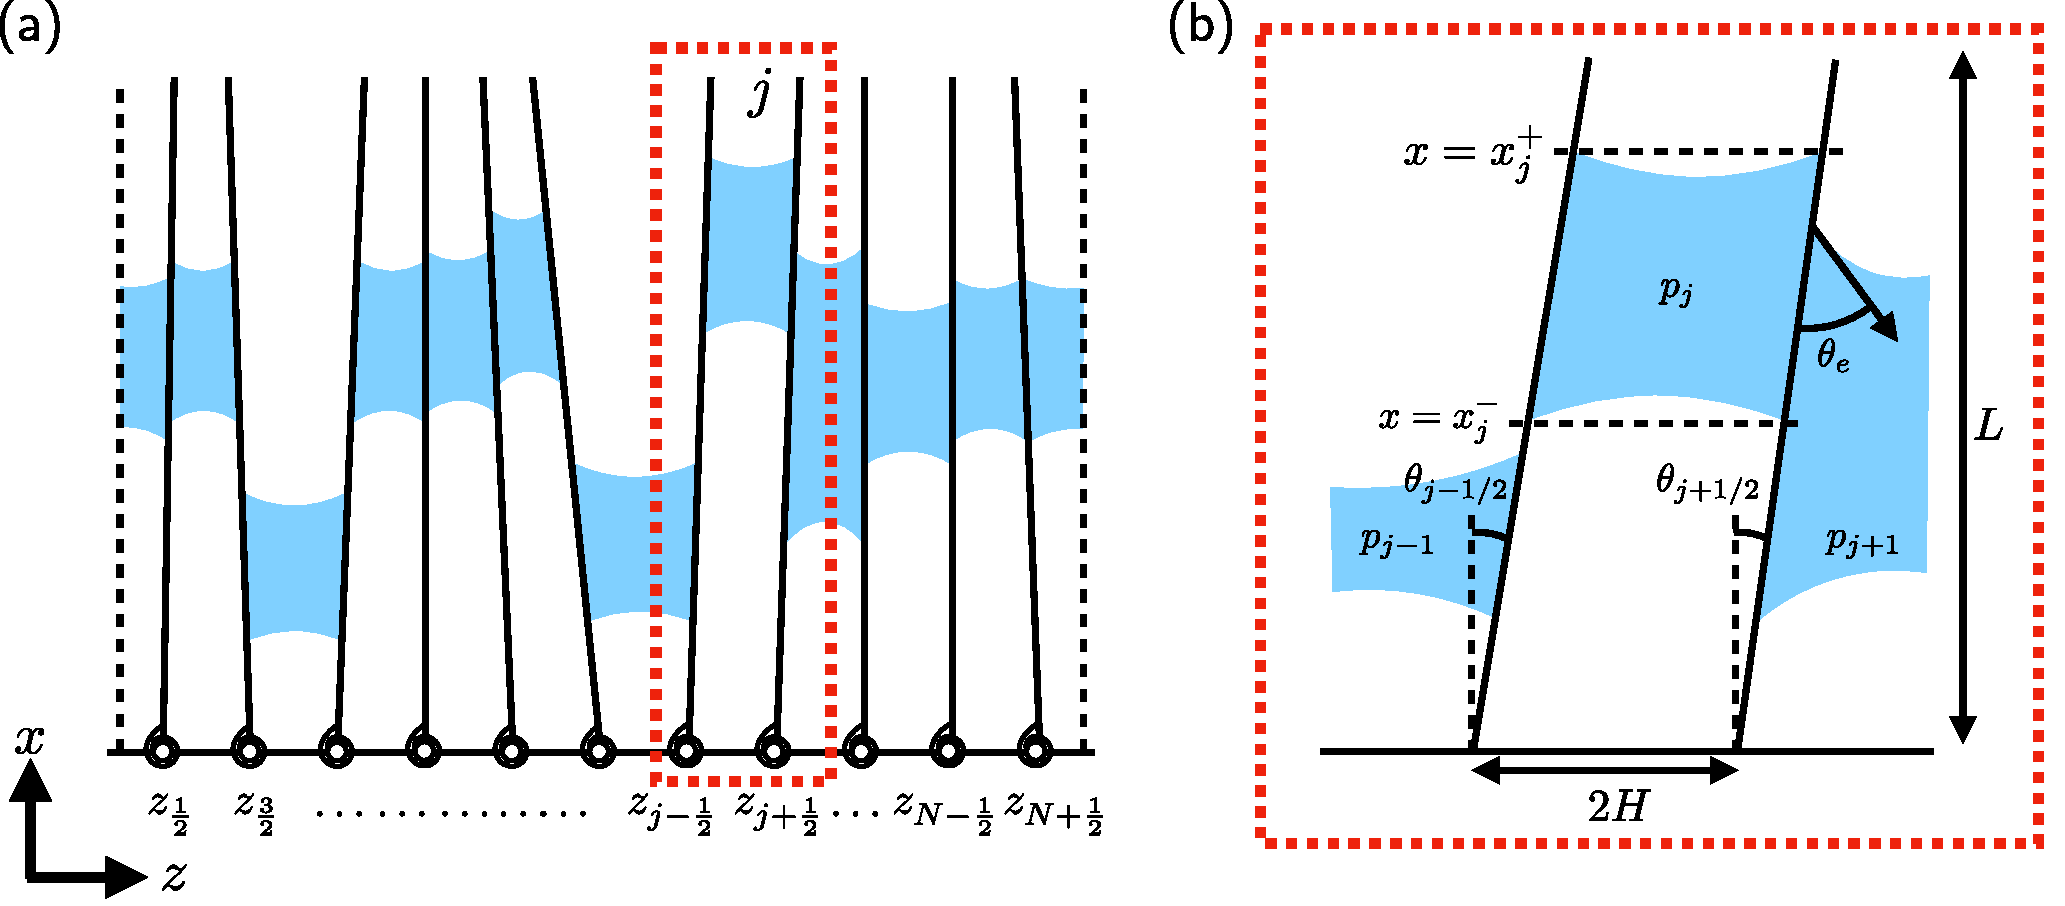
\includegraphics[width =0.95\textwidth]{SchematicMultiplePlates.pdf}
\caption{Modelling setup for interacting drop-channel systems. (a) Schematic diagram of the system of $N+1$ rigid plates, anchored at their base by torsion springs. (b) Detailed view of a single channel in the system. Note that the channel shape is described entriely by the adjacent deflection angles $\theta_{j-1/2}$ and $ \theta_{j+1/2}$.}\label{fig:Model:schematic}
\end{figure}

Each plate is anchored at a point along the $z$-axis, denoted $z = z_{j+1/2} = 2H(j+1/2),~j = 0,\dots, N$, by a torsion spring of stiffness $\kappa$ (this is consistent with channels of undeformed width $2H$ since the plates are assumed to be thin in comparison).  The torsion springs respond to applied torques by varying the angles (measured clockwise) they make with the $x$-axis; these are referred to as deflection angles, and are denoted by $\theta_{j+1/2}(t)$. The width of the $j^{\th}$ channel, at a perpendicular distance $x$ from its base is
\begin{equation}\label{E:Model:Modelling:ChannelWidth_withangles}
h_j(x,t) = 2H + x\tan\left( \theta_{j+1/2}\right) -x\tan \left(\theta_{j-1/2}\right),
\end{equation}
valid for $0 < x < L$. Note that the deflection angles scale with the channel aspect ratio $\alpha  = H/L \ll L $ so  changes in channel length in the $x$-direction because of plate tilting are negligible in comparison with $L$. This assumption also means that the channel widths can be approximated as
\begin{equation}\label{E:Model:Modelling:ChannelWidth}
h_j(x,t) = 2H + x \dthetaj(t)
\end{equation}
for $j = 1,\dots, N$, where $\dthetaj  = \theta_{j+1/2} - \theta_{j-1/2}$ denotes the tapering angle of the $j^{\text{th}}$ channel. Henceforth, the range of the index $j$ is suppressed -- it is always $j = 1,\dots, N$ -- and periodic conditions are assumed: any quantity with subscript $ 0$ or $N+1$ takes the same value as that quantity with subscript $N$ and $1$, respectively.

Droplets have (two-dimensional) volumes denoted by $V_j$ and make a liquid bridge between the channel walls. The $j^{\th}$ droplet wets the channel over the region $\xleftj(t)< x < \xrightj(t)$. (Note that whilst the channels are not necessarily symmetric about their midpoint -- $\theta_{j-1/2} \neq \theta_{j+1/2}$ in general -- it is consistent to assume that the meniscus positions are equal on each wall of the channel, as the deflection angles are small and the channel width thus varies slowly along its length.)

\subsection{Fluid Motion}
As before, lubrication theory is used to model the motion of the droplet. The pressure within the droplet in the $j^{\text{th}}$ gap, $p_j(x,t)$, satisfies Reynolds' equation~\citep{Leal2007}
\begin{equation}\label{E:Model:Modelling:ReynoldsEq}
 \ddp{h_j}{t}= x \ddp{\dthetaj}{t}= \ddp{}{x}\left[\frac{h_j^3}{12 \mu}\ddp{p_j}{x}\right] \quad \text{for} ~\xleftj(t)< x <\xrightj(t).
\end{equation}

For simplicity, we assume that condensation is negligible. As a result,  the flux of fluid through the menisci must balance that caused by the motion, giving the kinematic conditions
\begin{equation}\label{E:Model:Modelling:kinematic}
\dd{x^{\pm}_j}{t} = -\left.\frac{h_j(x_j^{\pm},t)^2}{12\mu}\ddp{p_{j}}{x}\right|_{x = x^{\pm}_j}.
\end{equation}

To solve~\eqref{E:Model:Modelling:ReynoldsEq} for the pressure within each drop, boundary conditions are required. There is a pressure jump across each meniscus caused by surface tension: as gravity is negligible, the menisci are arcs of circles whose curvature is $ 2\cos \theta_e/h_{j}(x_{\pm}^j,t)$ to leading order in $\alpha$ (the contribution to meniscus curvature from deflection angles comes in at $\mathcal{O}(\alpha)$). Taking the ambient pressure as reference, the liquid pressures at the menisci are therefore
\abeqn{E:Model:Modelling:laplace}{p_{j}(x^{+}_j, t) =- \frac{2\gamma \cos \theta_e}{2H + x_{+}^j \dthetaj},\qquad p_{j}(x^{-}_j, t) =- \frac{2\gamma \cos \theta_e}{2H + x_{-}^j \dthetaj}.}
Integrating equation~\eqref{E:Model:Modelling:ReynoldsEq} twice, using~\eqref{E:Model:Modelling:kinematic} and~\eqref{E:Model:Modelling:laplace} for the boundary terms, gives the $p_j$ in terms of $\dthetaj$, $\xbarj$, and their derivatives (see Appendix~\ref{Appendix:Reduction}).

\subsubsection{Pinned Drops}\label{S:Model:Model:Pinned}
During the motion, a droplet may reach the free end of the channel ($x = 1$) or the base ($x =0$). In practice, when it does so, the meniscus curvature relaxes by taking the value of the contact angle that ensures that the meniscus does not move (there is no flux of fluid there) until the contact angle has reached an advancing or receding angle (as discussed in detail for bendotaxis in a single flexible channel in Chapter 4). Here we have assumed, however, that the contact angle is fixed; we therefore encode pinned conditions by prescribing a no-flux condition instead of a Laplace pressure condition when the droplet is pinned. Explicitly, if the $j^\text{th}$ drop reaches the free end, we replace~\eqref{E:Model:Modelling:laplace}a with
\begin{equation}\label{E:Model:Modelling:kinematicPinned1}
\ddp{p_j}{x} = 0 \qquad \text{at}~x = x_j^+ = 1.
\end{equation}
so that by~\eqref{E:Model:Modelling:kinematic}, we have
\begin{equation}\label{E:Model:Modelling:kinematicPinned2}
\dd{\xrightj}{t} = 0,
\end{equation}
meaning that the meniscus does not subsequently move, and the droplet is said to be pinned. (Note that regardless of the droplet's pressure, it cannot be `unpinned', which may occur in practice as we saw in Chapter 4.)

Similarly, if the $j^\text{th}$ drop reaches the base, we replace \eqref{E:Model:Modelling:laplace}b by
\begin{equation}\label{E:Model:Modelling:kinematicPinned3}
\ddp{p_j}{x} = 0 \qquad \text{at}~x = x_j^- = 0,
\end{equation}
and hence $x_j^- = 0$ in the subsequent motion. We are, however, primarily interested in the behaviour before droplets are pinned, so consider boundary conditions~\eqref{E:Model:Modelling:kinematic}--\eqref{E:Model:Modelling:laplace} to be the default, which hold henceforth unless otherwise specified.

\subsection{Torque balance}
The pressure within each droplet has thus been determined (from~\eqref{E:Model:Modelling:ReynoldsEq}--\eqref{E:Model:Modelling:laplace}) in terms of the tapering angles, $\theta_{j+1/2}$,  the meniscus positions, $x_j^{\pm}$, and the time derivatives of both of these. To find a relationship between tapering and meniscus positions, a torque balance on each plate is considered.

Each plate is subject to torques from the liquid pressure within drops in the neighbouring channels, from interactions with neighbouring plates, and from the restoring spring torque. The fluid pressure torque on the $(j+1/2)^{\th}$ plate is
\begin{equation}\label{E:Model:Modelling:LaplaceTorque}
\tau_{\text{L}}^{j+1/2} = \int^{\xrightj}_{\xleftj} x p_{j}~\mathrm{d}x -  \int^{\xrightjj}_{\xleftjj} x p_{j+1}~\mathrm{d}x.
\end{equation}
\subsubsection{Plate contact}
For the case of flexible channel walls, considered in Chapter 2--4, there were two scenarios when the walls came into contact: regime II (making contact at a single point) and regime III (making contact along a portion of their length). However, for rigid plates, whose slopes are constant along their length, regime III has no analogue, so we model plate-plate interactions in a different way -- by including a van der Waals force between the plates. This force acts to repel beams strongly when they come close to touching (we also include a weak attraction to avoid bouncing out of contact). We assume that the van der Waals force is a point force on the end of the plates. The long range attraction and short range repulsion -- which prevents channel widths reaching zero -- is captured (see Figure~\ref{fig:Model:vanderWaals}) by taking the magnitude of the van der Waals forces between the $(j-1/2)^{\th}$ and $(j+1/2)^{\th}$ plates to be
\begin{equation}\label{E:Model:Modelling:vdwForce}
F_{j}(t) = A\left[\left(\frac{2H \varepsilon}{h_j(x = L,t)}\right)^9 - \left(\frac{2H\varepsilon }{h_j(x = L,t)}\right)^3\right],
\end{equation}
where $A$ is a constant force which sets the scale of plate-plate interaction forces and $\varepsilon$ is a small positive number (the equilibrium separation caused by van der Waals forces alone is $2H \varepsilon \ll 2H$).

\begin{figure}[t]
\centering
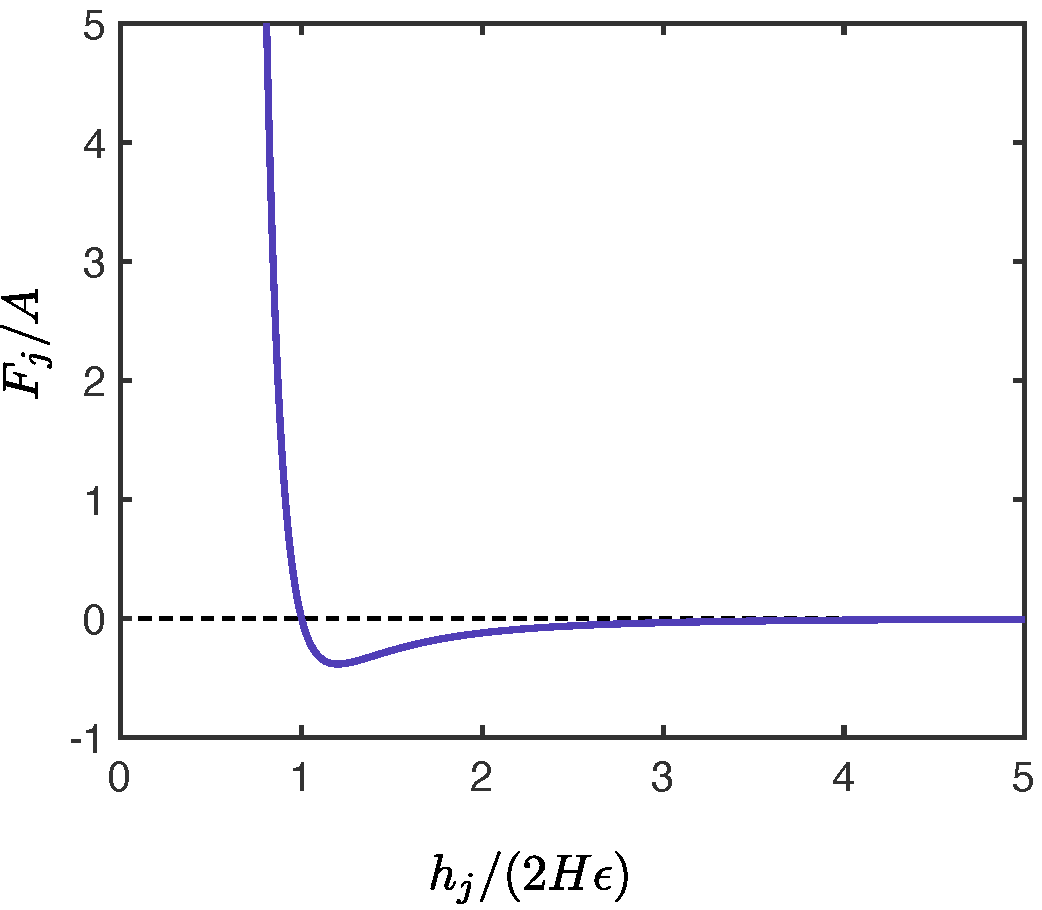
\includegraphics[scale=0.4]{vanderWaals}
\caption{Plot of the dimensionless function $F_j/A$ defined in equation~\eqref{E:Model:Modelling:vdwForce}. }\label{fig:Model:vanderWaals}
\end{figure}

The torque on the $(j+1/2)^{\th}$ plate due to van der Waals forces is then
\begin{equation}\label{E:Model:Modelling:vdwTorque}
 \tau^{\text{vdW}}_{j+1/2} = L\left[F_j(t) - F_{j+1}(t) \right].
\end{equation}

%Note that, provided it is weakly attractive at long range and strongly repulsive at short range, the particular expression for the van der Waals torque is unimportant and does not significantly alter the results of this chapter (appendix~\ref{Appendix:vanderWaals}).
\subsubsection{Torque balance equation}
The van der Waals and pressure-induced torques must be balanced by elasticity -- here represented by the restoring torque from the torsion spring. For a Hookean torsion spring, the restorative torque exerted on the $(j + 1/2)^\text{th}$ plate is
\begin{equation}\label{E:Model:Modelling:restorativeTorque}
\tau_{H}^{j+1/2} = \kappa \theta_{j+1/2}.
\end{equation}

A balance between damping within the spring and restorative torque, and van der Waals and fluid pressure torques gives
\begin{equation}\label{E:Model:Modelling:torqueBalance}
C_{\text{p}}\dd{\theta_{j+1/2}}{t} + \kappa \theta_{j+1/2}=\int^{\xrightj}_{\xleftj} x p_{j}~\mathrm{d}x -  \int^{\xrightjj}_{\xleftjj} x p_{j+1}~\mathrm{d}x + \tau^{\text{vdW}}_{j+1/2}
\end{equation}
where $C_{\text{p}}$ is the angular damping coefficient of the spring. Here  the particular form of the van der Waals torques has been  suppressed to reflect its unimportance (it is the characteristic short range repulsion and long range attraction, rather than the exact expression, of the van der Waals term that is important).

\subsection{Initial conditions}\label{S:Model:InitialConditions}
The system of differential equations is closed by specifying initial conditions
\begin{equation}\label{E:Model:Modelling:InitialConditions}
\xrightj(0) = x_{j,0}^{+}, \quad \xleftj(0) = x_{j,0}^{-}, \quad \theta_{j+1/2}(0) = \theta_{j+1/2}^0.
\end{equation}
These initial conditions implicitly specify the drop volumes, which must be conserved throughout the motion. Neglecting the missing volume contribution from the arc of the meniscus (which scales with the channel aspect ration $\alpha \ll 1$), conservation of volume can be expressed as $\mathrm{d}V_j/\mathrm{d}t = 0$, where
\begin{equation}\label{E:Model:Modelling:Volumes}
V_j = \left[\xrightj(t) - \xleftj(t)\right]\frac{h_j(\xrightj,t) + h_j(\xleftj,t)}{2}.
\end{equation}
(Note that $\mathrm{d}V_j/\mathrm{d}t = 0$ holds automatically when the kinematic conditions~\eqref{E:Model:Modelling:kinematic} hold).
\subsection{Non-dimensionalization}\label{S:Model:NonDim}
We non-dimensionalize the problem by choosing scales for spatial variables that are motivated by the channel geometry. The time scale emerges from of a balance between viscosity and capillarity, as before. In particular, we let
\begin{align}\label{E:Model:NonDim:Scales1}
\hat{t} &= \frac{H |\gamma \cos \theta_e|} {\mu L^2}t, &  (\hat{x},\hat{x}_j^{\pm})&= \frac{1}{L}(x,x_{j}^{\pm}), & \hat{h}_j &= \frac{1}{2H}h_j,
\end{align}
where dimensionless variables are denoted by $\hat{\cdot}$. In each of the models we have developed so far in this thesis, we have taken a  pressure scale that is set by a balance between beam bending and Laplace pressure. The equivalent scaling in this torsion spring model is that obtained by balancing the restorative spring torque and the fluid pressure torques in equation~\eqref{E:Model:Modelling:torqueBalance}; we therefore let
\begin{equation}\label{E:Model:NonDim:PressureScaling}
\hat{p}_j = \frac{L^3}{ 2H \kappa}p_j.
\end{equation}
Note that, in contrast to the flexible case, the behaviour of the whole, rather than half, of the channel is modelled -- this difference is responsible for the apparent extra factor of two. The torques generated by plate interactions are non-dimensionalized by scaling with the typical scale of the restoring torque scale, $2H\kappa/L$, i.e.
\begin{equation}\label{E:Model:NonDim:BeamInteractionTorqueScaling}
\hat{\tau}_{j+1/2}^{\text{vdW}} = \frac{L}{2H \kappa} \tau_{j+1/2}^{\text{vdW}}.
\end{equation}
Deflection angles are scaled by the aspect ratio, i.e. we let
\begin{equation}\label{E:Model:NonDim:AngleScaling}
\hat{\theta}_{j+1/2} = \frac{L}{2H}{\theta}_{j+1/2},
\end{equation}
and the dimensionless channel tapering is $\Delta \hat{\theta}_{j} = \hat{\theta}_{j+1/2} - \hat{\theta}_{j-1/2}$. The dimensionless channel widths are then
\begin{equation}\label{E:Model:NonDim:DimensionlessChannelWidth}
\hat{h}_j(x,t) = 1 + \hat{x}\Delta \hat{\theta}_{j}.
\end{equation}


\subsection{Statement of the problem}
In terms of these scaled variables, Reynolds' equation~\eqref{E:Model:Modelling:ReynoldsEq} reads
\begin{equation}\label{E:Model:NonDim:ReynoldsEq}
 \hat{x} \ddp{ \Delta \hat{\theta}_{j}}{\hat{t}}= \frac{1}{3|\Gamma|}\ddp{}{\hat{x}}\left[\hat{h}_j^3\ddp{\hat{p}_j}{\hat{x}}\right] \qquad \text{for} ~~\hat{x}_{-}^j(\hat{t})< \hat{x} <\hat{x}_{+}^j(\hat{t}).
\end{equation}
Here
\begin{equation}\label{E:Model:NonDim:GammaDefinition}
\Gamma = \frac{\gamma \cos \theta_e L^3}{2 \kappa H^2}
\end{equation}
is the dimensionless surface tension, which compares the typical torque from surface tension, $L^2\gamma/H$, with the typical restoring torque from the torsional spring $\kappa H/L$. The parameter $\Gamma$ is analogous to the bendability $\nu$ we have considered throughout this thesis. Different wettability conditions are captured by the sign of $\Gamma$: $\Gamma > 0$ corresponds to a droplet that wets the channel walls ($\theta_e < \pi/2$), and $\Gamma < 0$ to a droplet that does not ($\theta_e > \pi/2$).

Inserting~\eqref{E:Model:NonDim:Scales1}--\eqref{E:Model:NonDim:DimensionlessChannelWidth} in the kinematic conditions~\eqref{E:Model:Modelling:kinematic} and pressure boundary conditions~\eqref{E:Model:Modelling:laplace} gives
\begin{equation}\label{E:Model:NonDim:Kinematic}
\dd{\hat{x}_j^{\pm}}{\hat{t}} = -\frac{\hat{h}_j^2}{3|\Gamma|}\left.\ddp{\hat{p}_j}{\hat{x}}\right|_{\hat{x} = \hat{x}_{j}^{\pm}},
\end{equation}
and
\begin{equation}\label{E:Model:NonDim:Laplace}
\hat{p}_j(\hat{x}_{j}^{\pm}, \hat{t}) = -\frac{\Gamma}{1 + \hat{x}_j^{\pm}\Delta \hat{\theta}_j},
\end{equation}
respectively.

The torque balance becomes
\begin{equation}\label{E:Model:NonDim:TorqueBalance}
\hat{C}_p\dd{\hat{\theta}_{j+1/2}}{\hat{t}} + \hat{\theta}_{j+1/2} = \int_{x_{j}^{-}}^{x_{j}^{+}}\hat{x}\hat{p}_j ~\mathrm{d}x - \int_{x_{j+1}^{-}}^{x_{j+1}^{+}}\hat{x}\hat{p}_{j+1} ~\mathrm{d}x + \hat{\tau}_{j+1/2}^{\text{VDW}}
\end{equation}
where $\hat{C}_p= C_p H |\gamma \cos \theta_e|/(\mu \kappa L)$ is a dimensionless damping coefficient. We are primarily interested in the case where the dissipation occurs mainly due to the droplet viscosity, i.e. $\hat{C}_p \ll 1$; nevertheless, we retain the first term in~\eqref{E:Model:NonDim:TorqueBalance} due its importance in numerically solving the system (this is discussed further in \S\ref{S:Numerics}).  Note that this droplet-dominated dissipation is in contrast to previous torsion spring models of elastocapillary aggregation~\citep{Wei2014EPL, Wei2015PRSA} where configurations with wall-dominated damping, $\hat{C}_p\gg 1$, are considered. In~\eqref{E:Model:NonDim:TorqueBalance}, the dimensionless van der Waals torque is
\begin{equation}
\hat{\tau}_{j+1/2}^{\text{vdW}} = \hat{F}_{j} - \hat{F}_{j+1}
\end{equation}
where
\begin{equation}
\hat{F}_{j} = \frac{AL}{2H \kappa}\left[\left(\frac{\varepsilon}{\hat{h}_j(\hat{x} = 1, \hat{t})}\right)^9 -\left(\frac{\varepsilon}{\hat{h}_j(\hat{x} = 1, \hat{t})}\right)^3 \right]
\end{equation}
is the dimensionless van der Waals force between the $(j-1/2)^{\th}$ and $(j+1/2)^{\th}$ plates. The quantity $AL/(2H\kappa)$ compares a typical torque from the interaction between two plates separated by an $\mathcal{O}(\varepsilon)$ distance, with the typical restoring force from the torsion spring. To ensure van der Waals forces only become important for channels whose walls are very close to one another, we consider $AL/(2H\kappa) \ll 1$ here (we take $AL/(2H\kappa) = 10^{-6}$, $\varepsilon = 10^{-2}$ in all results presented in this chapter).

The dimensionless initial conditions,
\begin{equation}\label{E:Model:NonDim:InitialConditions}
\hat{x}_{j}^{\pm}(0) = \hat{x}_{j, 0}^{\pm}, \qquad \hat{\theta}_{j+1/2}(0) = \hat{\theta}_{j+1/2}^0,
\end{equation}
close the problem~\eqref{E:Model:NonDim:ReynoldsEq},~\eqref{E:Model:NonDim:TorqueBalance}--\eqref{E:Model:NonDim:Volume}, and also define the dimensionless droplet volumes
\begin{equation}\label{E:Model:NonDim:Volume}
\frac{V_j}{2HL} = \hat{V}_j = \left(\hat{x}_{j,0}^+ -\hat{x}_{j,0}^-\right))\frac{2 + \left(\hat{\theta}_{j+1}-\hat{\theta}_{j,0}\right) \left(\hat{x}_j^+ + \hat{x}_{j,0}^-\right)}{2},
\end{equation}
which represents the proportion of the channel a given drop would occupy if its walls were undeformed. Hats are henceforth dropped, and all quantities are dimensionless unless otherwise stated.

\subsection{System of differential equations}
It is convenient to work in terms of the mean meniscus position and drop half length, defined as
\begin{equation}\label{E:Model:DAEs:Definition_xbar_ell}
\xbarj = \frac{\xleftj + \xrightj}{2}\quad \text{and}\quad \ellj = \frac{\xrightj - \xleftj}{2}
\end{equation}
respectively. The meniscus positions are easily recovered from these as
\begin{equation}
\xrightj = \xbarj + \ellj, \quad \xleftj = \xbarj - \ellj.
\end{equation}
Equations~\eqref{E:Model:NonDim:ReynoldsEq}--\eqref{E:Model:NonDim:InitialConditions} can be reduced to a system of $2N$ ordinary differential equations (ODEs) for $\theta_{j+1/2}, \xbar_j$. Briefly (see Appendix~\ref{Appendix:Reduction} for further details), we first note that mass conservation requires
\begin{equation}\label{E:Model:DAEs:CoMass}
V_j = 2\ell_j(1 + \xbarj\dthetaj),
\end{equation}
to be constant throughout, which gives the droplet lengths $\ellj$ algebraically in terms of the $\xbar_j$ and $\Delta \theta_{j}$. We then integrate Reynolds' equation~\eqref{E:Model:NonDim:ReynoldsEq} twice alongside the Laplace pressure conditions~\eqref{E:Model:NonDim:Laplace} to obtain an expression for droplet pressures $p_j$ in terms of $\xbar_j, \Delta \theta_j$ and $\mathrm{d}(\Delta \theta_j)/\mathrm{d}t$. Inserting this expression into the torque balance equation~\eqref{E:Model:NonDim:TorqueBalance} gives the following $N$ ODEs:
\begin{multline}
-C_p\dd{\theta_{j+1/2}}{t} +|\Gamma|\left( \viscdamp_{j+1}\dd{\Delta \theta_{j+1}}{t} -  \viscdamp_{j}\dd{\Delta \theta_{j}}{t}\right) =\\
\theta_{j+1/2} - \tau^{\text{vdW}}_{j+1/2} + \frac{\Gamma}{2}\left[\frac{2\ell_{j}\Delta \theta_{j}I^2_j}{ h_j^+ h_j^-I^0_j} - \frac{2\ell_{j+1}\Delta \theta_{j+1}I^2_{j+1}}{ h_{j+1}^+ h_{j+1}^-I^0_{j+1}} -\right. \\
\left.\frac{(\bar{x}_{j+1}+\ell_{j+1})^2}{h_{j+1}^+} - \frac{(\bar{x}_{j+1}-\ell_{j+1})^2}{h_{j+1}^-} - \frac{(\bar{x}_{j}+\ell_{j})^2}{h_{j}^+} + \frac{(\bar{x}_{j}-\ell_{j})^2}{h_{j}^-}\right].\label{E:Model:DAEs:TorqueBal}
\end{multline}
Here the integrals $I_j^0, I_j^2,$ and $I_j^4$ are defined by
\begin{equation}\label{E:Model:DAEs:InDefinition}
I_j^n(t) = \int_{\xbar_j - \ell_j}^{\xbar_j + \ell_j} \frac{x^n}{(1 + x\dthetaj)^3}~\mathrm{d}x, ~n \in \mathbb{N}.
\end{equation}
The quantities
\begin{equation}\label{E:Model:DAEs:ViscDampDefn}
\viscdamp_j = \int_{\xbarj - \ellj}^{\xbarj + \ellj}\frac{x^2}{2}\ddp{p_j}{x}~\mathrm{d}x=  \frac{3}{4I^0_j}\left[I^0_j I^4_j - \left(I^2_j\right)^2\right].
\end{equation}
play the role of viscous dissipation in the droplet.

Inserting the expression for the pressure into the kinematic conditions~\eqref{E:Model:NonDim:Kinematic} (and taking their sum) gives $N$ ODEs:
\begin{multline}\label{E:Model:DAEs:Kinematic}
2\dd{\xbarj}{t}  +\frac{1}{2} \left[\frac{\ellj^2 + 2\ellj \xbarj}{h_j^+} + \frac{\ellj^2 - 2\ellj \xbarj}{h_j^-} -  \frac{I_2^j - \xbar_j^2 I_0^j}{I_0^j} \left(\frac{1}{h_j^+} + \frac{1}{h_j^-}\right)\right]\dd{(\dthetaj)}{t} =\\
-\frac{2\ellj\dthetaj\sgn(\Gamma)}{3I_0^j h_j^+ h_j^-} \left(\frac{1}{h_j^+} + \frac{1}{h_j^-}\right).
\end{multline}
The ODEs~\eqref{E:Model:DAEs:Kinematic} capture the balance between the two modes of droplet transport: squeezing (via the $\mathrm{d}(\dthetaj)/\mathrm{d}t$) and translating (via the $\mathrm{d}\xbarj/\mathrm{d}t$).

The differential equations~\eqref{E:Model:DAEs:TorqueBal} and~\eqref{E:Model:DAEs:Kinematic} are solved alongside the initial conditions
\begin{equation}\label{E:Model:DAEs:IC}
\theta_{j+1/2}(0) = \theta_{j+1/2}^0,\quad \xbar_j(0) =\xbar_j^0  = \frac{x_{j,0}^+ + x_{j,0}^-}{2},
\end{equation}
(Note that the procedure, and resulting differential equation system, is slightly different if droplets are pinned at the end of their channels -- see Appendix~\ref{Appendix:Reduction}.)


\section{The single channel case}\label{S:SingleChannel}
Having developed a model capable of describing bendotaxis in many interacting channels, we consider first the description of a droplet in a single channel. There are two reasons for studying this system: firstly it will allow us to verify that the equations derived in \S\ref{S:Model} (i.e. with torsion springs and rigid plates, rather than flexible plates as in Chapter 2--4) do indeed exhibit droplet transport to the free end of a single channel, regardless of wettability. The other reason is that by comparing the two models (flexible response and torsion spring response), information is gleaned about the relationship between the bending stiffness of beams in a flexible system, and the torsion stiffness included in the present system.  We would  like to keep our torsion spring model as faithful as possible to a model with flexible channel walls (which we expect to be more appropriate for describing a physical system). It might be expected that an appropriate choice of torsion stiffness would give quantitative agreement between the two models, giving greater confidence in the validity of results of this chapter when describing an array of flexible channels.

\subsection{Governing equations and numerical Solutions}
\begin{figure}[t]
\centering
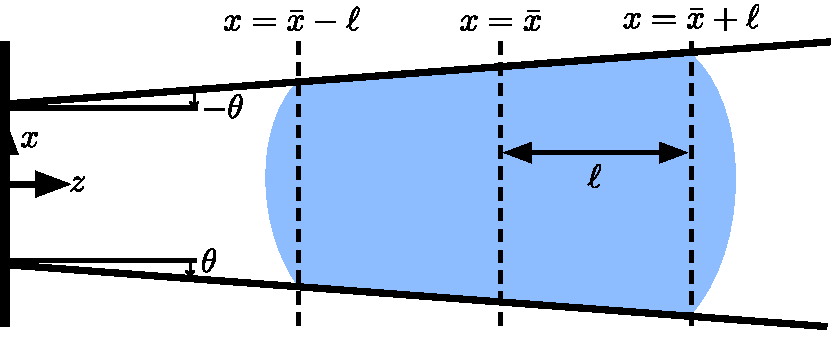
\includegraphics[scale=0.6]{SchematicSingleChannel_noghost.pdf}
\caption{Schematic diagram of a non-wetting droplet in a channel whose rigid walls are tethered at their base with torsion springs. Arrows indicate the clockwise direction in which angles are measured, i.e. $-\theta$ denotes an angle of magnitude $\theta$ measured anticlockwise about the $x$-axis.}\label{fig:SingleChannel:Schematic}
\end{figure}

A single drop-channel system is equivalent to the periodic system described in \S\ref{S:Model} with $N =2$ channels, one of which (say $j = 2$) contains a drop of trivial length (i.e. $\ell_2 = 0$). In this case, only one angle, $\theta_{3/2} = \theta$, needs to be considered; the other angles are $\theta_{1/2} = -\theta$ (by symmetry), and $\theta_{5/2} = -\theta$ (by periodicity), with the angle difference $\Delta \theta_{1} = 2\theta$ (see Figure~\ref{fig:SingleChannel:Schematic}). The system is described entirely by the angle $\theta$ and mean position $\xbar_1 = \xbar$ of the non-trivial drop. The droplet volume is $V\coloneqq V_1$ and is treated as a known parameter, and the droplet half length is $\ell = V/\left[2(1 + \xbar\Delta \theta)\right]$.

(Note that with this periodic formulation, it is possible that results for non-wetting drops with strong surface tension -- $\Gamma < 0$ with $|\Gamma| \gg 1$ -- may be unintentionally affected by van der Waals interactions between the beams which define the `ghost' channel containing no drop. This is resolved in what follows by including only van der Waals interactions between the beams surrounding the drop.



With these simplifications equations~\eqref{E:Model:DAEs:TorqueBal} and~\eqref{E:Model:DAEs:Kinematic} become (with suppressed indices):
\begin{align}
2\dd{\xbar}{t}+ \left[\frac{\ell^2 - 2\ell \xbar}{h^-} + \frac{\ell^2 + 2\ell \xbar}{h^+}-\frac{2(\xbar^2 I^0 - I^2)\bar{h}}{I^0 h^+ h^-}  \right]\dd{\theta}{t} +\frac{8\ell \theta\sgn (\Gamma)\bar{h}}{3I^0(h^+)^2 (h^+)^2} &= 0, \label{E:TwoPlates:DAEs1}\\
-2\left(C_p+|\Gamma|\viscdamp\right)\dd{\theta}{t}- \theta + \tau^{\text{vdW}} - \frac{\Gamma}{2}\left[\frac{4\ell \theta I^2}{I^0 h^+ h^-} + \frac{(\xbar + \ell)^2}{h^+} - \frac{(\xbar - \ell)^2}{h^-}\right]&=0\label{E:TwoPlates:DAEs2}
\end{align}
where $h^{\pm} = 1 + (\xbar \pm \ell)\Delta \theta, ~\bar{h} = 1 + \xbar\Delta \theta$ are the channel widths at the menisci and at the mean meniscus position, respectively. The system~\eqref{E:TwoPlates:DAEs1}--\eqref{E:TwoPlates:DAEs2} is closed by specifying initial conditions
\begin{equation}\label{E:TwoPlates:IC}
\xbar(0) = \xbar_0, \qquad \theta(0) = \theta_0.
\end{equation}

Figure~\ref{fig:TwoPlates:NumSols} shows traces of meniscus positions $x^{\pm} = \xbar \pm \ell$ and channel tapering $\Delta \theta$, obtained by solving equations~\eqref{E:TwoPlates:DAEs1}--\eqref{E:TwoPlates:DAEs2} numerically using the stiff ODE solver \textsc{ODE15s} implemented in \textsc{matlab}. As discussed in Chapter 2 for the flexible case, a stiff solver is required because of the different time scales present: as $\theta_0 = 0$, the beams offer no restoring force to balance the capillary pressure to begin with, so there is a short time scale on which damping from droplet viscosity must balance the capillary torque. During this short time scale, the droplet does not move very far -- it ultimately moves on a longer time scale during which the torsion spring resistance is important (these time scales are formally distinguishable in the case of weak surface tension, discussed later in this section). This early response can be seen in numerical solutions: see Figure~\ref{fig:TwoPlates:NumSols}, for example, in which the deflection angle in a numerical solution of~\eqref{E:TwoPlates:DAEs1}--\eqref{E:TwoPlates:DAEs2} with $\Gamma = 5$ reaches 90$\%$ of its final value in less than $1\%$ of the time taken for the droplet to reach the end of the channel. As we shall see, this separation of timescale is even more pronounced for $\Gamma = 0.1$ but is not resolved on the scale of Figure~\ref{fig:TwoPlates:NumSols}.

\begin{figure}[h!]
\centering
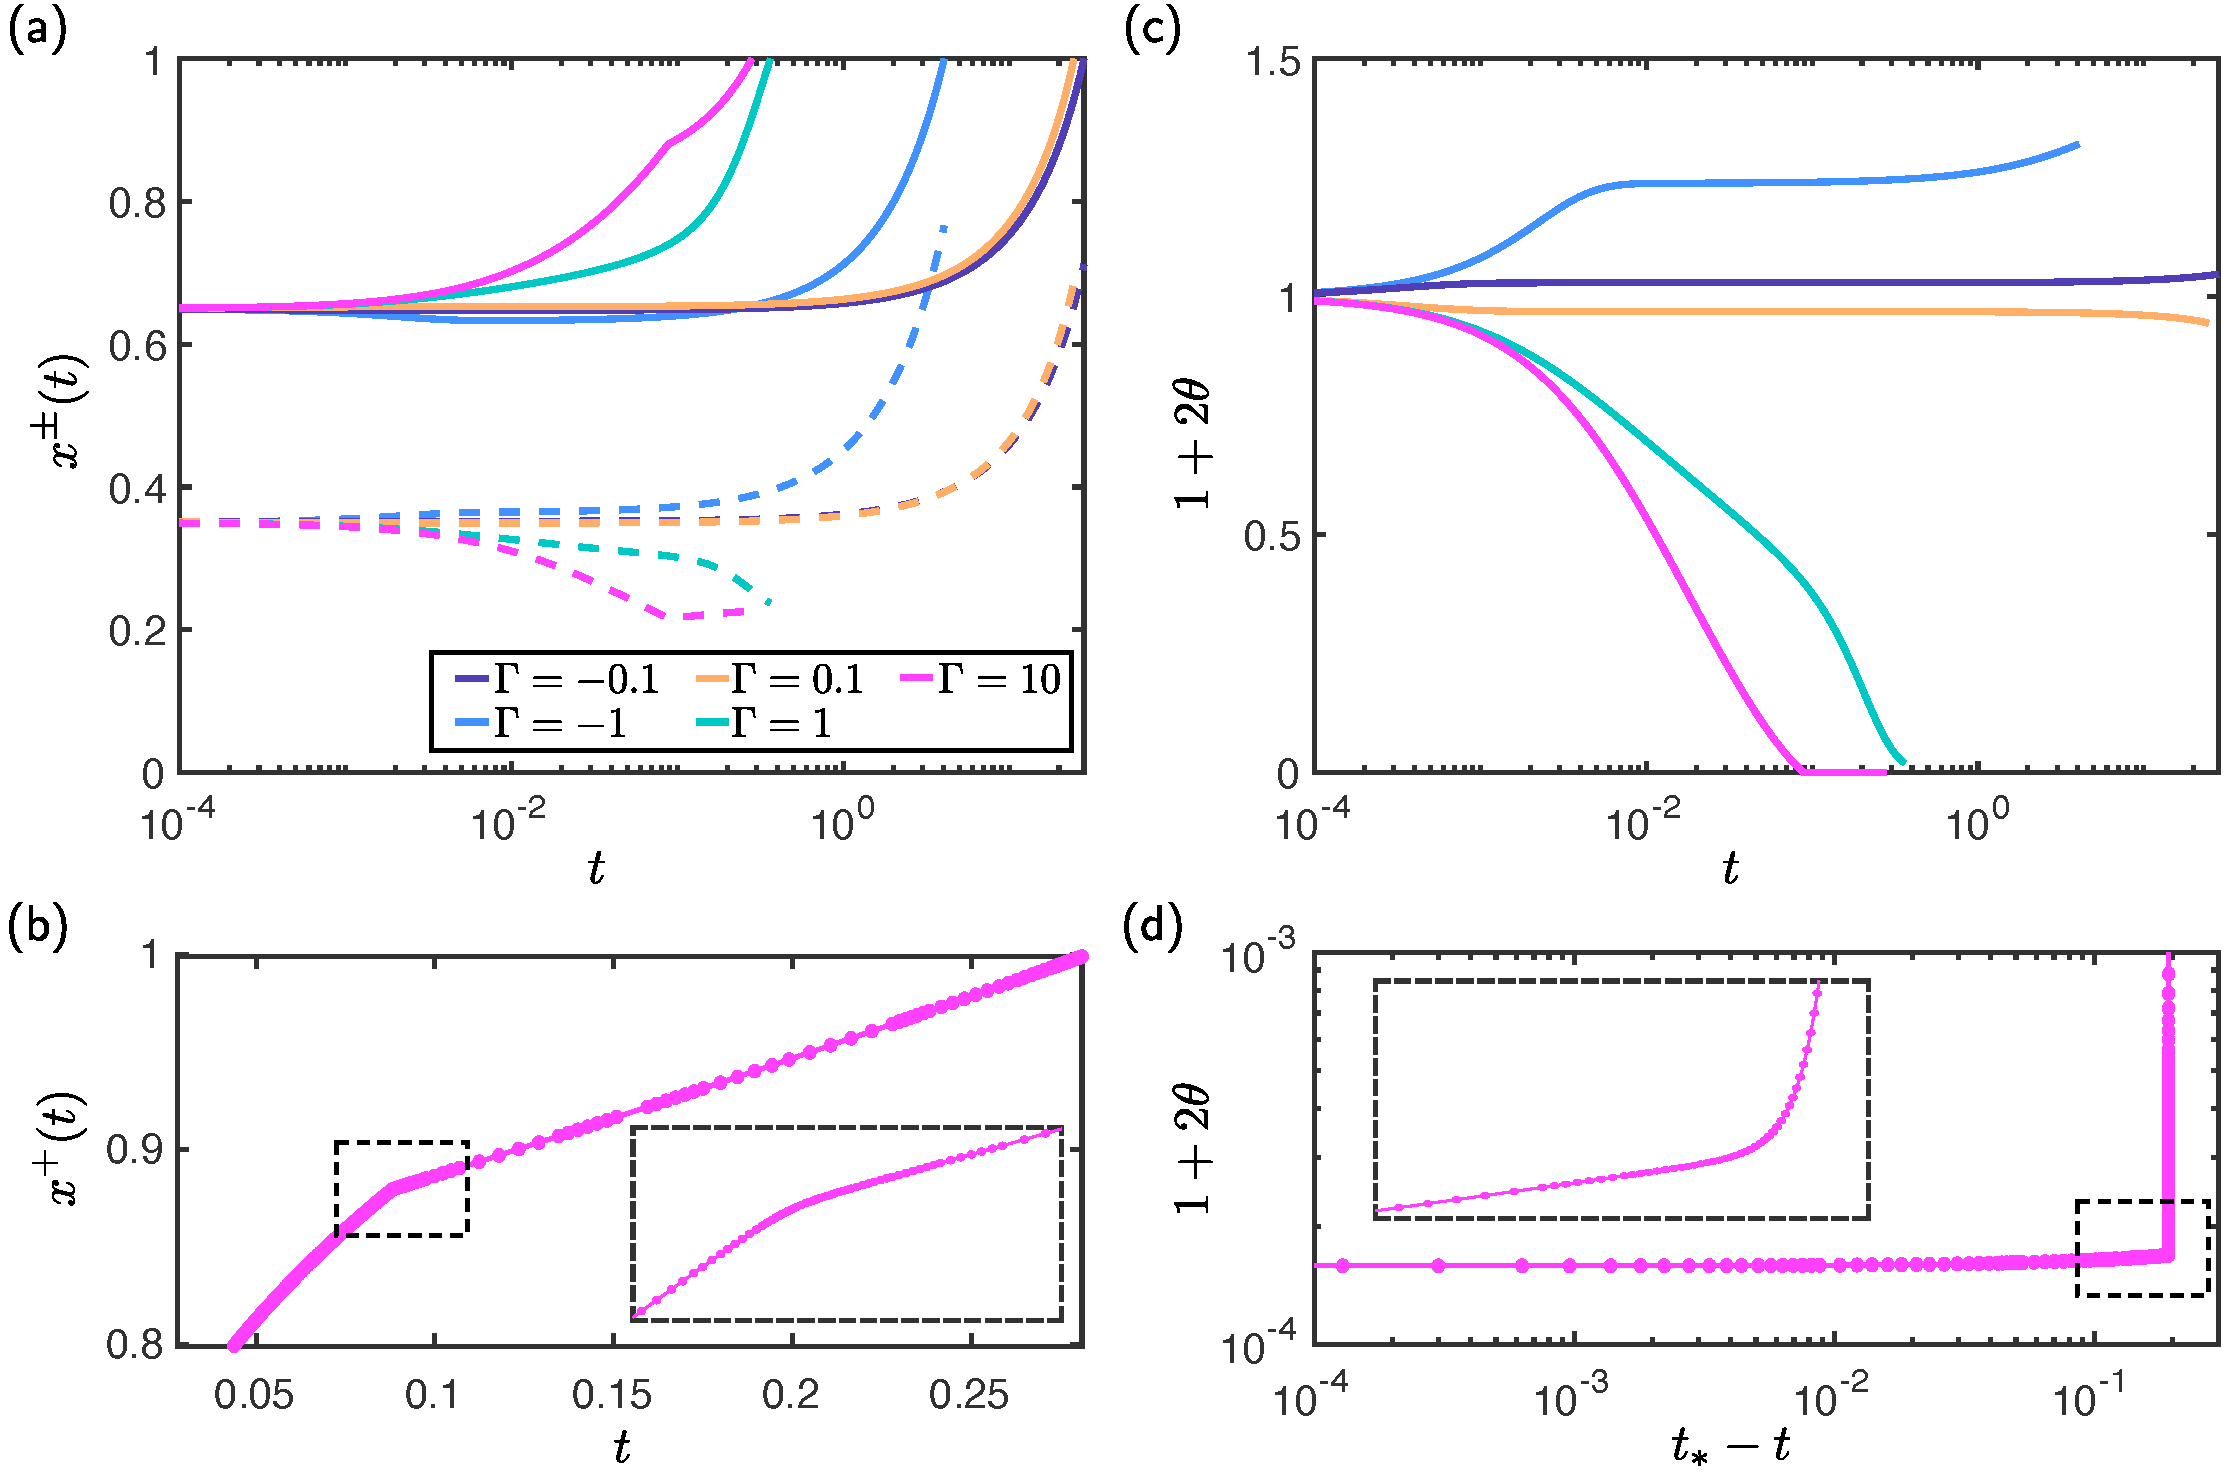
\includegraphics[width = 0.95\textwidth]{Traces_menisci_and_tapering.pdf}
\caption{Numerically-obtained solutions of equations~\eqref{E:TwoPlates:DAEs1}--\eqref{E:TwoPlates:DAEs2} with $\theta_0 = 0, \xbar_0 = 0.5$ and $V = 0.3$. (a): Traces of $x^{+} = \xbar+\ell$ (solid lines) and $x^{-} = \xbar-\ell$ (dashed lines) plotted on semi-logarithmic axes for four values of the dimensionless surface tension $\Gamma$ as indicated by the legend. The traces end when $x^+ = 1$, denoted $t =t_*$. (b): Portion of the  $\Gamma = 10$ trace indicated by the black dashed box in (a) (plotted on linear axes) showing constant velocity motion into the wedge. The rapid change in slope occurs when the plate ends are sufficiently close for van der Waals forces to be significant ($1 + 2\theta \approx 0$). Points indicate the mesh (in time) used in the numerical solution. The inset shows the behaviour close to the rapid change in speed, indicating that the traces shown in (a) and (b) are well resolved. (c): Traces of the channel width at the free end, $1 + 2 \theta$ on semi-logarithmic axes (colours are as in (a)). (d) Plot of channel width as a function of $t_* -t$ on logarithmic axes, corresponding to the region shown by the black dashed box in (c) with dots again indicating the mesh in time. Note that the channel does not close entirely, $1 + 2\theta >0$ (the distance at which van der Waals force is zero is taken to be $10^{-3}$). Inset: zoomed in on region indicated by the black box in (c), demonstrating that the channel width is also well resolved.}
\label{fig:TwoPlates:NumSols}
\end{figure}

These numerical solutions demonstrate that the model described in \S\ref{S:Model} describes droplet transport by bendotaxis in a single channel that is wettability independent (in this case, the `bending' occurs in the torsion spring, rather than in the channel walls): droplets are transported to the free end (the trajectories $x^{+}(t)$ shown in Figure~\ref{fig:TwoPlates:NumSols}(a) reach $x = 1$) regardless of whether the droplets wet the channel ($\Gamma > 0$) or not ($\Gamma < 0$), a result that is generic in numerical solutions of~\eqref{E:TwoPlates:DAEs1}--\eqref{E:TwoPlates:DAEs2} (provided droplets do not start too close to the base and make contact during the early time scale, where menisci move in opposite directions). This droplet motion is accompanied by an inwards deflection when the droplets wets the channel ($\Delta \theta = 2\theta <0$ in Figure~\ref{fig:TwoPlates:NumSols}(b)) and outwards when it does not ($\Delta \theta = 2\theta >0$), as we also saw in the flexible case. There are further similarities: droplets accelerate along the channel, and beam-beam interactions play a role when surface tension is sufficiently strong: the magenta traces ($\Gamma = 10$) in Figure~\ref{fig:TwoPlates:NumSols} show that the `+' meniscus decelerates briefly at $t\approx 10^{-1}$, when the channel walls come sufficiently close for van der Waals force to be important. The short range repulsion associated with this force means the channel does not close entirely (Figure~\ref{fig:TwoPlates:NumSols}(d)) but forms a triangle-like wedge (albeit with a narrow gap). This is in contrast to the flexible case considered in Chapters 2--4, where the beams make contact. It might be expected that the lubrication approximation breaks down as the droplet moves into this wedge, but we note that the constant speed of imbibition into it (Figure~\ref{fig:TwoPlates:NumSols}(b)) is consistent with theory and experiment describing the similar scenario of droplet imbibition into rigid wedges~\citep{Reyssat2014JFM}.




\subsection{Comparison between torsion spring and flexible cases}\label{S:SingleChannel:FlexibleComparison}
As discussed, we would like our torsion spring model, in which the spring stiffness $\kappa$ is known, to be as faithful as possible to a flexible model whose walls have a bending stiffness $B$. However, we would prefer to use the torsion spring model for multibody bendotaxis due to its relative simplicity. We therefore want to find an effective spring stiffness -- the value of $\kappa$ that gives quantitative agreement with the flexible case for a given value of $B$.

Note that $\kappa$ has the units of a force, while $B$ has the units of a force per unit length, so they must be related via a length scale. The present problem has two geometric length scales, $L$ and $H$ as well as the length scales defined by the position of the drop, say $X_d$, and the length of the drop (denoted $\Delta X$ in Chapters 2--4). It is not immediately obvious which is the correct choice. Here, we compare the results of a single channel to those of the flexible model described in Chapter 2 in the case of weak surface tension, $|\Gamma| \ll 1$, where analytic results can be found in both the flexible and torsion spring cases. In doing so, we identify the correct length scale and offer a suggestion on how to choose an effective spring stiffness.

The asymptotic analysis of equations~\eqref{E:TwoPlates:DAEs1}--\eqref{E:TwoPlates:DAEs2} in the limit $|\Gamma |\ll 1$ (see Appendix~\ref{Appendix:SmallGammaAnalysis} for full details) begins by assuming small deformations $|\theta| \ll 1$ for all $t>0$. The dynamics then decouple into two distinct time scales: on a fast ($\mathcal{O}(\Gamma)$) timescale, the drop does not make a net movement along the channel ($\xbar$ is constant), but the deflection angles respond to applied torques. At early times, this response arises from a torque imbalance: no resistive torque is offered by the torsion springs since $\theta_0 = 0$, but there is a non-trivial capillary pressure which must therefore be balanced by dissipation in the drop and plate. The angle evolution is given by
\begin{equation}\label{E:SingleChannel:SmallGamma:FastTimescaleEq}
\theta = -\Gamma V \xbar_0\left[1 - \exp\left(\frac{-1}{C_p + C_{d}^0}\frac{t}{|\Gamma|}\right)\right],
\end{equation}
where
\begin{equation}\label{E:SingleChannel:SmallGamma:SlowTimescaleEq}
C_{d}^0 = V^3\left(\frac{V^2}{240} + \frac{\xbar_0^2}{4}\right)
\end{equation}
is the leading-order term in the expansion of droplet dissipation for $|\Delta \theta| \ll 1$. The droplet itself moves on a long ($\mathcal{O}(1/|\Gamma|)$) timescale, with the mean meniscus position evolving according to the ODE
\begin{equation}\label{E:SingleChannel:SmallGamma:xbarODE}
\dd{\xbar}{t} = \frac{2|\Gamma|V}{3}\xbar.
\end{equation}
As discussed in Chapter 2, when the channel walls are flexible, and wall deflections are small, the droplet moves according to the ODE
\begin{equation}\label{E:SingleChannel:SmallGamma:xbarODE_flexible}
\dd{\xbar}{t} = \frac{|\nu| V}{6}\left(\xbar + \frac{V}{2}\right)^2.
\end{equation}
where $\nu = \gamma \cos \theta_e L^4/(BH^2)$.

Comparison of~\eqref{E:SingleChannel:SmallGamma:xbarODE} and~\eqref{E:SingleChannel:SmallGamma:xbarODE_flexible} suggests that the length scale relating $\kappa$ and $B$ is $X_d$, i.e. $\kappa \sim B/X_d$. This is perhaps unsurprising: in the flexible case, the further away from the clamped end that a (fixed) force is applied, the larger the deformation (note that this is necessary for bendotaxis to occur). Or, equivalently, two channels, whose flexible walls have different bending stiffnesses, may experience the same deformation from a droplet if it is father from the clamped end in the channel whose walls have a higher bending stiffness.

It is therefore not possible to find an `effective bending stiffness' which gives completely equivalent dynamic behaviour. However, we can find quantitative agreement between the flexible and torsion spring cases with respect to certain metrics (in the small $\Gamma$ limit). Here we consider one example: the time taken for the droplet to traverse a section of the between $x = f < 1$ and $x = 1$. This is the metric we used in our experimental study of bendotaxis in Chapter 3 as a proxy for the dynamic behaviour.

By solving the ODE~\eqref{E:SingleChannel:SmallGamma:xbarODE}, we find that the dimensionless bendotaxis time for a single torsion spring channel is
\begin{equation}\label{E:SingleChannel:SmallGamma:tX}
t_{f} = \frac{3}{2|\Gamma|V}\log\left(\frac{2-V}{2X-V}\right).
\end{equation}
In Chapter 2, we found the equivalent result for the flexible case:
\begin{equation}
t_{f}^{\text{flexible}} = \frac{6}{|\nu|V}\frac{1-f}{f}.
\end{equation}
Therefore quantitative agreement between the flexible and torsion spring cases (with respect to the bendotaxis time) can be had by considering a system whose spring stiffness is
\begin{equation}\label{E:SingleChannel:SmallGamma:EffectiveBending}
\kappa = \frac{2(1-f)}{f \log\left(\frac{2-V}{2f-V}\right)}\frac{B}{L}.
\end{equation}
In other words, the asymptotic results presented in Chapter 2 for a flexible channel of bending stiffness $B$ are identical to those for a torsion spring channel whose spring stiffness is chosen according to~\eqref{E:SingleChannel:SmallGamma:EffectiveBending}.



\section{Numerical solutions}\label{S:Numerics}
In this section, we present numerical solutions of the governing equations derived in \S\ref{S:Model}, and describe the numerical methods used to obtain them. Note that in the following sections (\S\ref{S:Numerics}--\S\ref{S:Discussion}), we consider only wetting drops ($\Gamma >0$); the corresponding results of these sections in the non-wetting case are discussed in \S\ref{S:NonWetting}.

\subsection{Details of numerical methods}\label{S:Numerics:Details}
To numerically solve the problem, we first express equations~\eqref{E:Model:DAEs:TorqueBal} and~\eqref{E:Model:DAEs:Kinematic} as a single matrix differential equation
\begin{equation}\label{E:NumSols:MDE:MatrixDifferentialEquation}
\underline{M}\dd{\underline{u}}{t} =\underline{f}.
\end{equation}
where $\underline{u} = (\theta_{3/2},\dots, \theta_{N+1/2},\xbar_1,\dots,\xbar_N)^\intercal$. Here $\underline{M}$ and $\underline{f}$ play the roles of a mass matrix and a force, respectively (note that $\underline{M}$ changes dynamically and captures pinning conditions, see Appendix~\ref{Appendix:MatrixDifferentialEquation} for more details, including explicit expressions for  $\underline{M}$ and $\underline{f}$). In this setting, the initial condition is
\begin{equation}\label{E:NumSols:MDE:IC}
\underline{u}^0 =\left(\theta_{3/2}^0, \dots, \theta_{N+1/2}^0,\xbar_1^0, \dots,\xbar_N^0\right)^\intercal.
\end{equation}

The matrix equation~\eqref{E:NumSols:MDE:MatrixDifferentialEquation} is  well-defined only if $\underline{M}$ has full rank. This is not the case when plate damping is neglected ($C_p = 0$); in this case, the first $N+1$ rows of $\underline{M}$ have zero row-sum, and hence $\underline{M}$ has a zero eigenvector $\underline{v}_0 =(1,\dots,1,0,\dots,0)^\intercal$. This elucidates the importance of retaining plate damping in the model.

Let us briefly consider $\underline{v}_0$: this eigenvector corresponds to increasing each of the deflection angles by an equal amount, without changing the positions or shapes -- and therefore capillary torques -- of the droplets. Increasing the deflection angles, however, increases the restoring torques from the torsion springs, resulting in a torque imbalance; when $C_p \neq 0$, this imbalance is resolved on a fast timescale where plate damping balances with restoring torque.

We therefore consider $0 < C_p \ll 1$  in the rest of this chapter (recall that the latter inequality ensures droplet damping dominates over plate damping). All results presented use $C_p= 10^{-3}$, but we have observed that numerical solutions display indistinguishable behaviour with $C_p = 10^{-5}, 10^{-4}$, and $10^{-3}$.

The problem~\eqref{E:NumSols:MDE:MatrixDifferentialEquation}--\eqref{E:NumSols:MDE:IC} is solved numerically using the \texttt{ODE15s} routine in \textsc{matlab}. At each time-step, the sparse mass matrix $\underline{M}$ is evaluated, with particular care taken in the computation of the integrals $I_j^n, n = 0,2,4$. Analytic expressions for the $I_j^n$ can be found for $|\dthetaj|>0$ by integrating~\eqref{E:Model:DAEs:InDefinition} by parts, and trivially for $\dthetaj=0$. This result is singular in the limit $|\dthetaj| \to 0$, so the $I_j^n$ are evaluated for $|\dthetaj|\ll 1$ by expanding the integrand in $|\dthetaj|$ and integrating term-by-term. (We are careful to ensure that the magnitude of errors introduced by truncating this sum fall below errors from numerical integration.)

\subsection{Numerical experiments}\label{S:Numerics:NumericalExperiments}
\begin{figure}[h!]
\centering
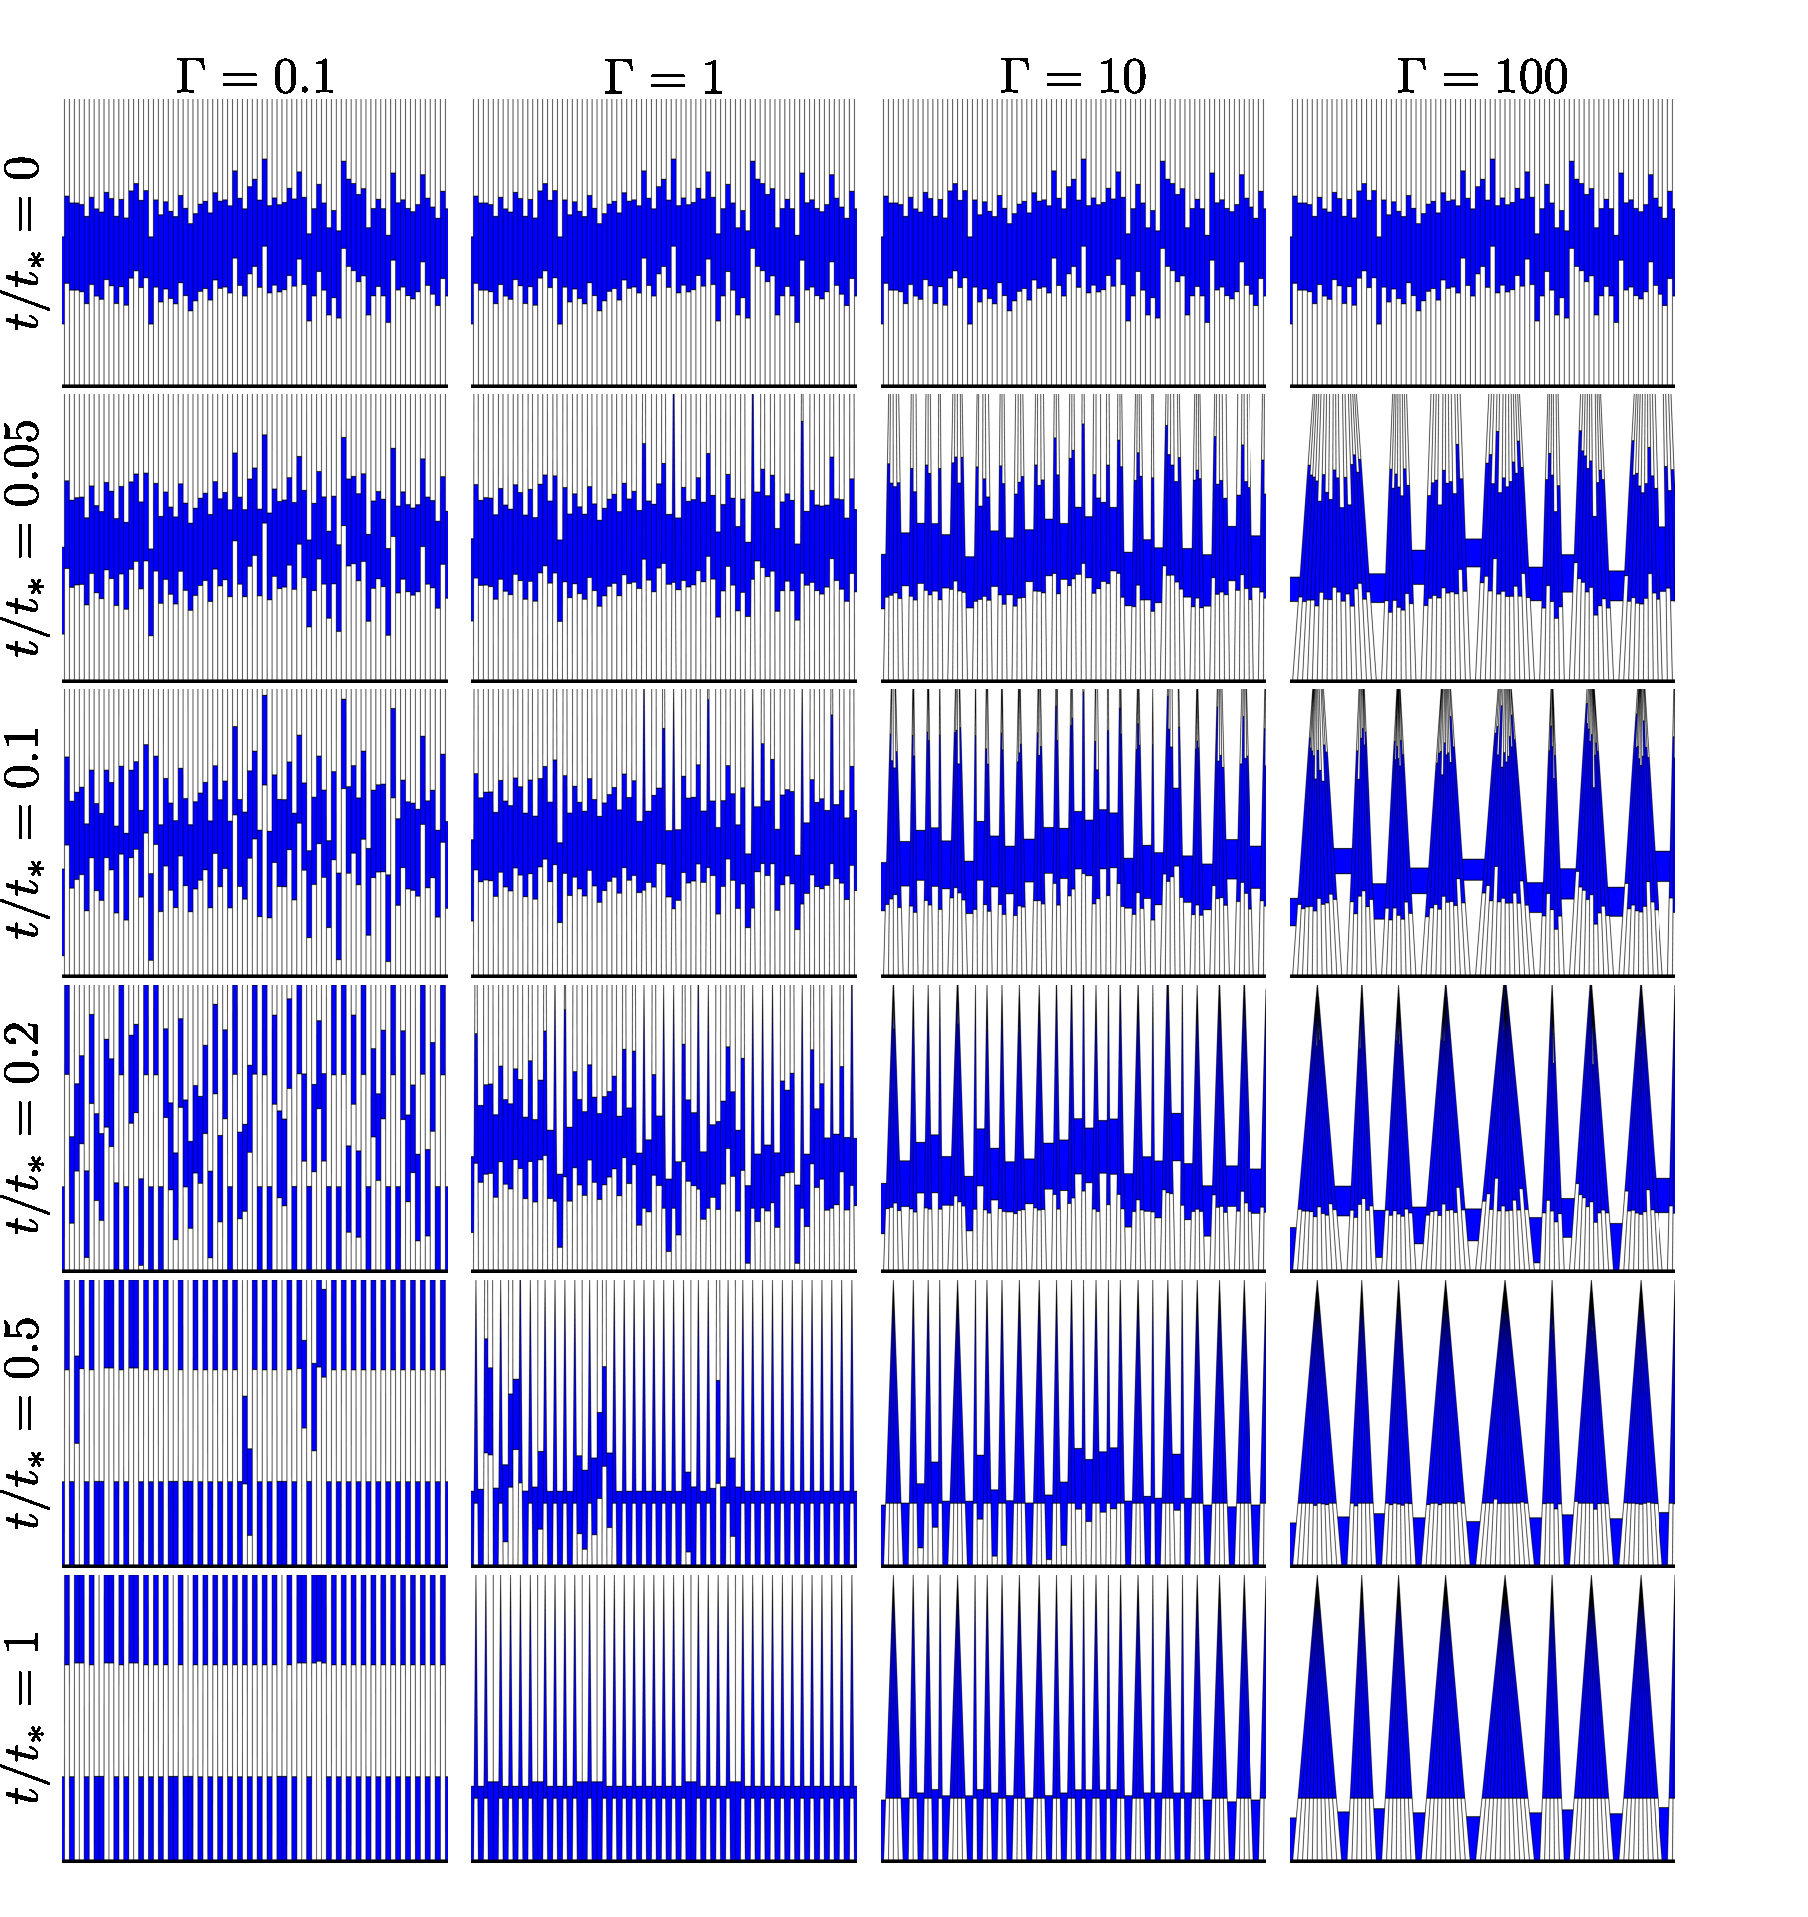
\includegraphics[width = \textwidth]{Snapshots.pdf}
\caption{Snapshots of arrays corresponding to numerical solutions of~\eqref{E:NumSols:MDE:MatrixDifferentialEquation} with random initial conditions~\eqref{E:Numerics:NumericalExperiments:RandomIC} (the initial conditions are the same for each value of $\Gamma$ with $\epsilon = 0.1$ and $\xbar_0 = 0.5$) and uniform volumes $V_j = 0.3$. The time at which the snapshot is taken is measured relative to $t_*$ -- the time at which every droplet has reached either end of the channel containing it. Here, $t_* \approx 300,~6,~1,~0.6$, for $\Gamma = 0.1,~1,~10,~100$ respectively. Note that the equations were solved for $N=199$ channels (i.e. $200$ plates), but only those with indices $1 < j < 80$ are shown here for clarity.}\label{fig:Numerics:Snapshots}
\end{figure}

\begin{figure}[t]
\centering
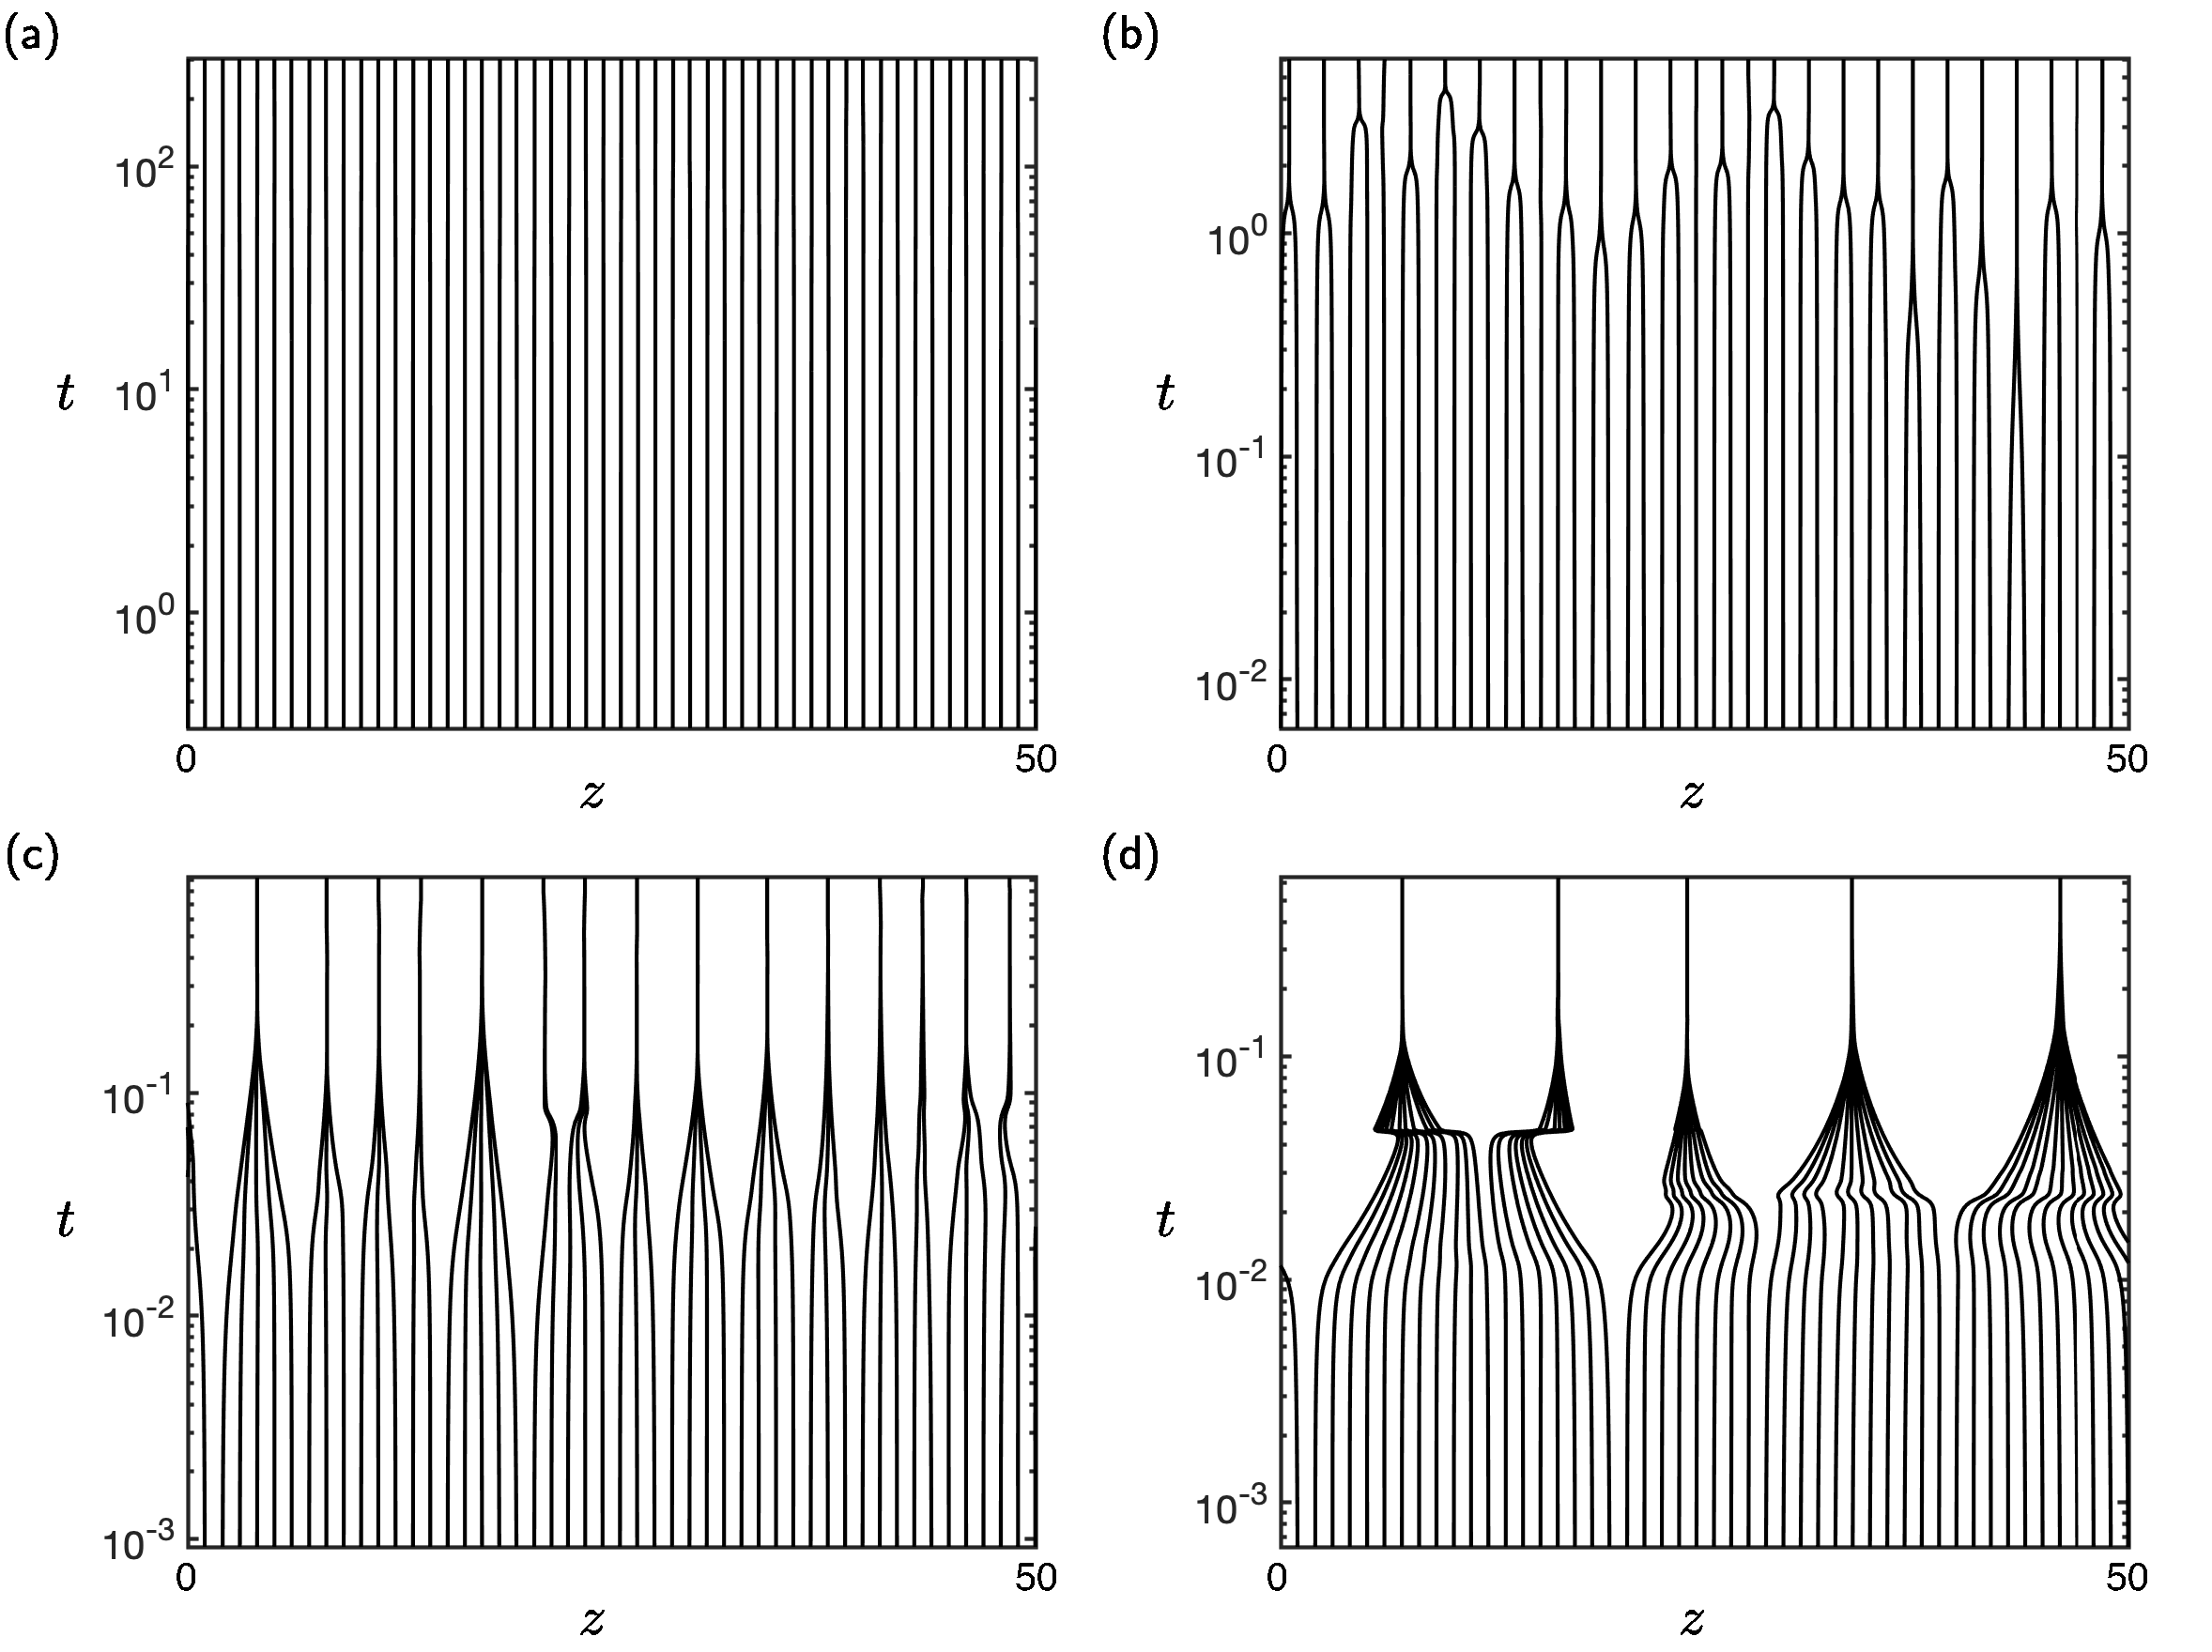
\includegraphics[width = \textwidth]{Spatiotemporal_combined.pdf}
\caption{Spatiotemporal plots of numerical solutions to~\eqref{E:NumSols:MDE:MatrixDifferentialEquation} with random initial conditions~\eqref{E:Numerics:NumericalExperiments:RandomIC} (with $\epsilon = 10^{-1}, \xbar_0 = 0.5$). Each subplot corresponds to a column of the snapshots displayed in Figure~\ref{fig:Numerics:Snapshots}, i.e. each  corresponds to a different value of $\Gamma$ as follows: (a) $\Gamma = 0.1$, (b) $\Gamma = 1$, (c) $\Gamma = 10$, (d) $\Gamma = 100$. Here $V_j = 0.3$, and $N=199$ channels consisting of $200$ plates (only 50 plates are shown for clarity).  Note that each curve in $(z,t)$ space corresponds to the trajectory of the end ($x=1$) of a single beam. The apparent kinks in (d) are the separation of large clusters into two smaller clusters (see main text).}\label{fig:Numerics:Spatiotemporal}
\end{figure}

\begin{figure}[t]
\centering
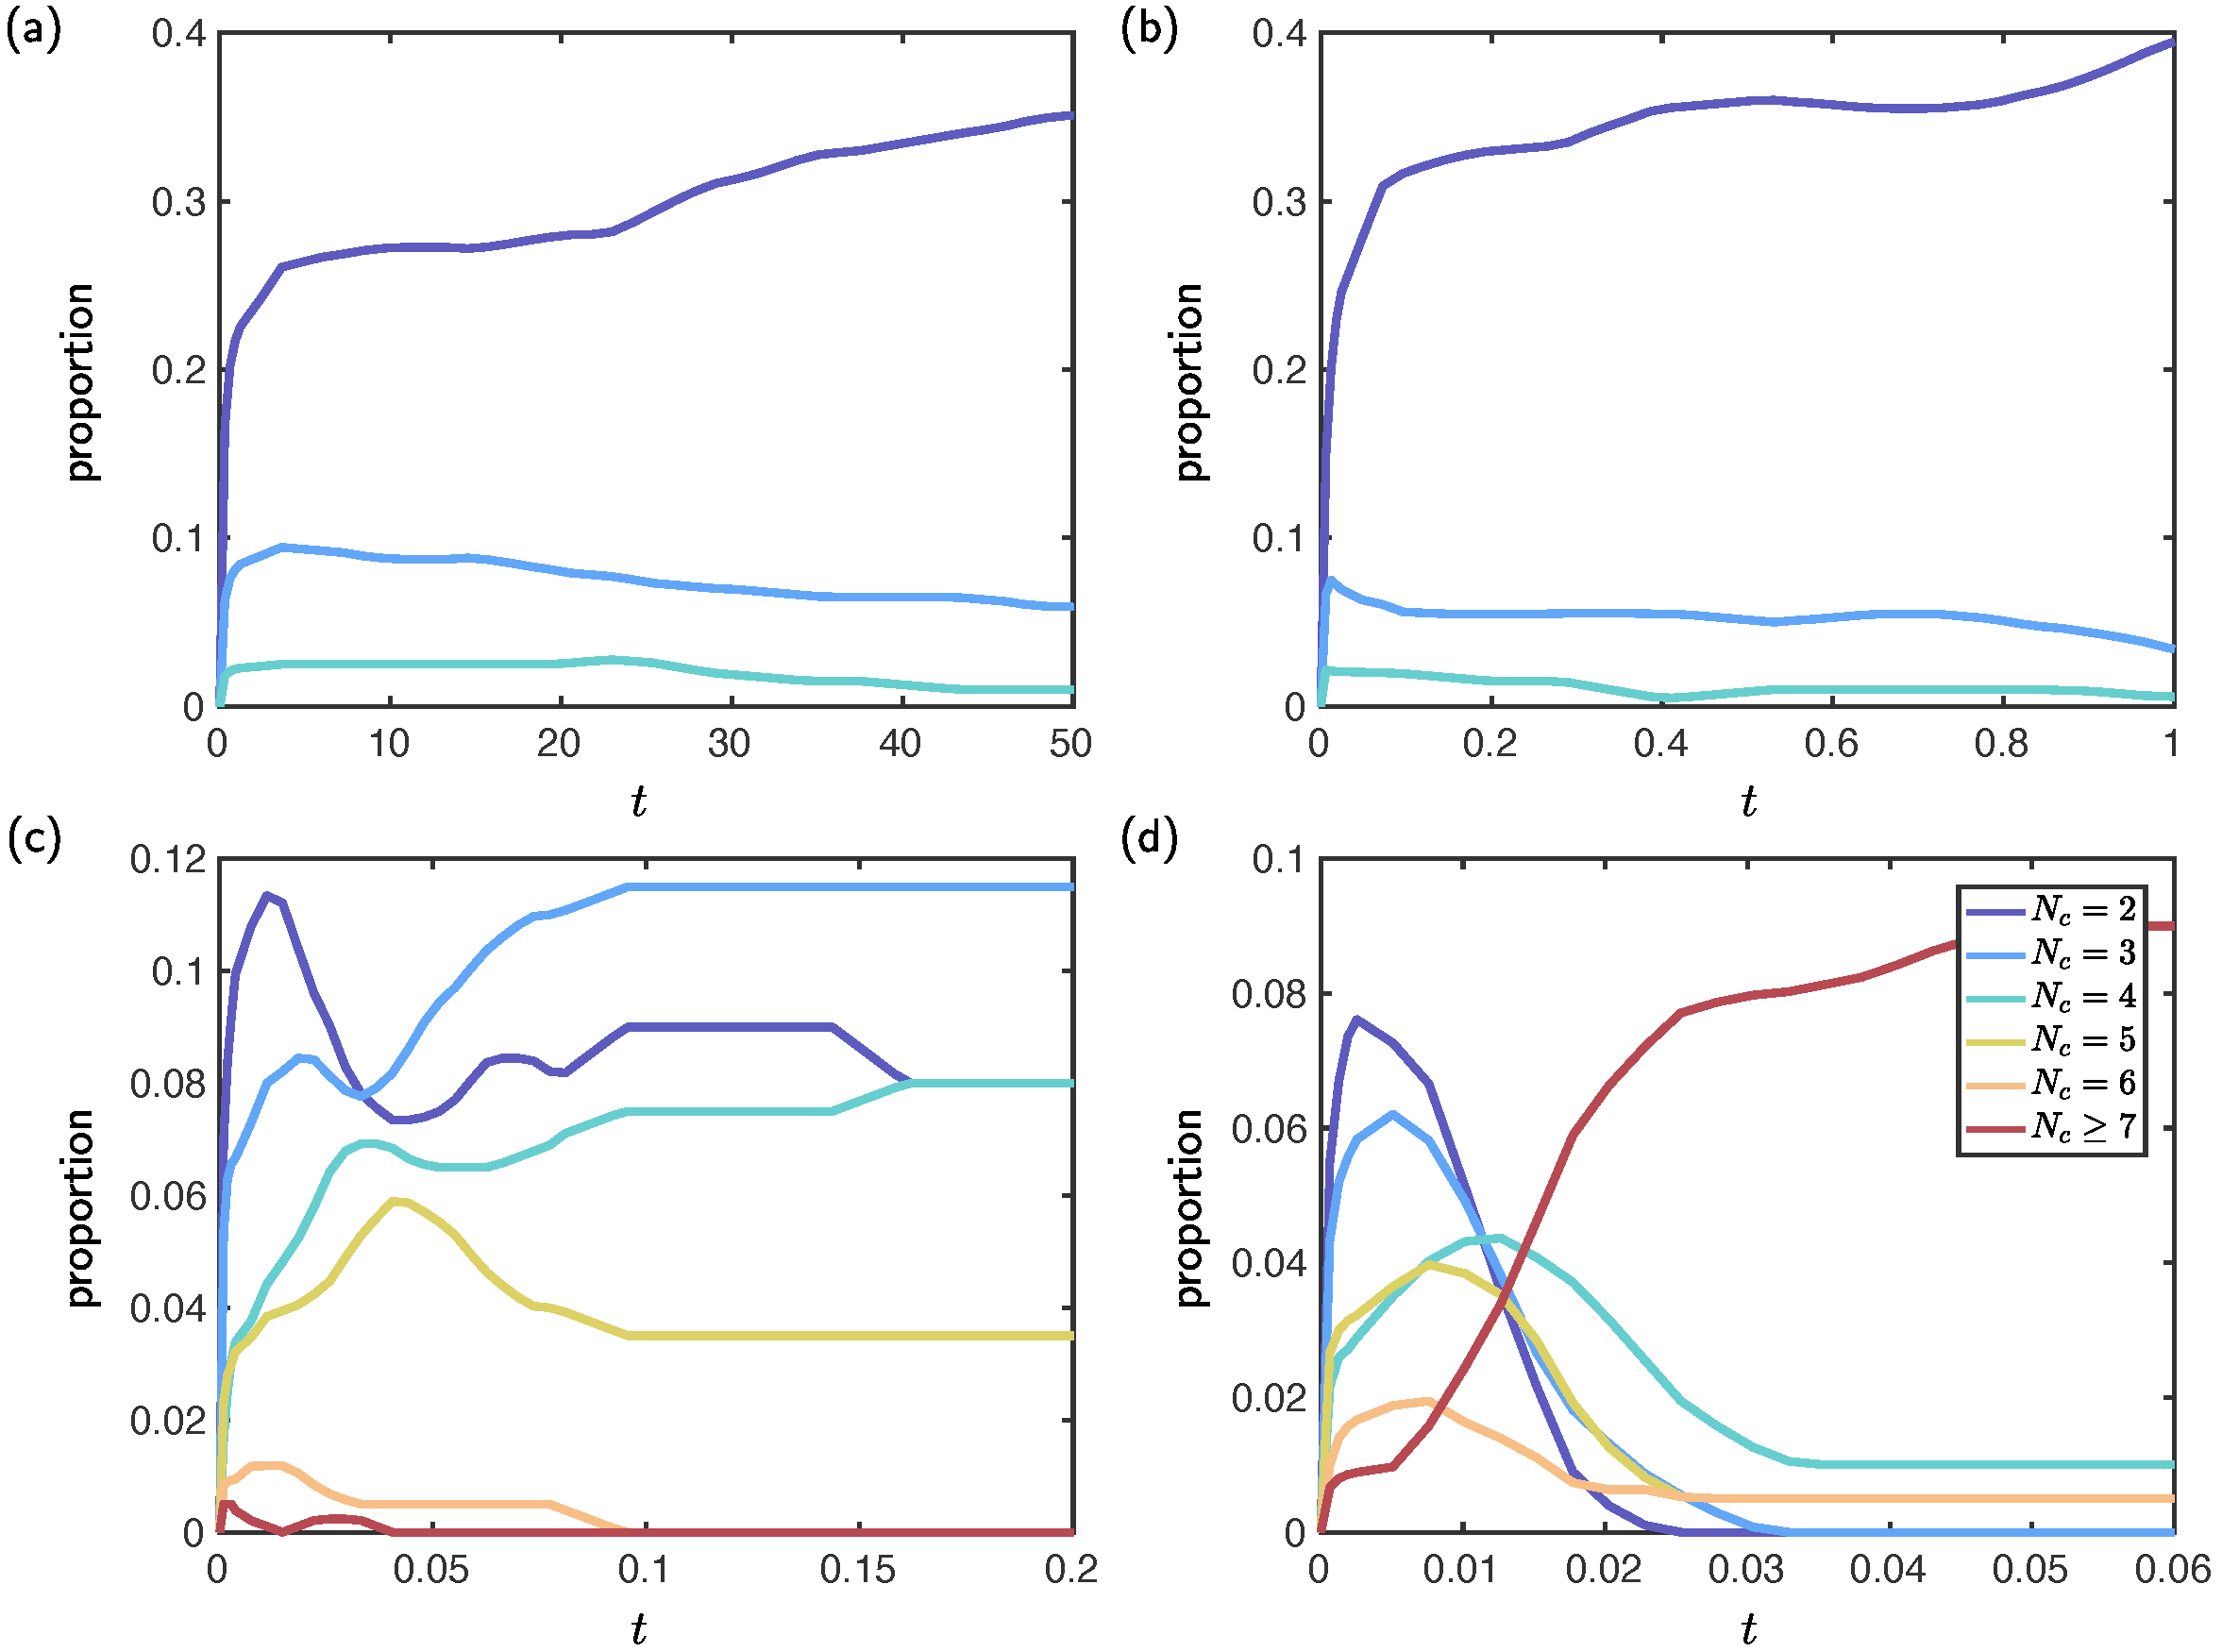
\includegraphics[width = 0.95\textwidth]{ClusterSizes}
\caption{Evolution of the proportion of clusters of each particular size $N_p$ (indicated in the legend in (d)) in numerical solutions~\eqref{E:NumSols:MDE:MatrixDifferentialEquation} with random initial conditions~\eqref{E:Numerics:NumericalExperiments:RandomIC}. Each subplot corresponds to a column of the snapshots, which are displayed in Figure~\ref{fig:Numerics:Snapshots}, i.e. each subplot corresponds to a different value of $\Gamma$ as follows: (a) $\Gamma = 0.1$, (b) $\Gamma = 1$, (c) $\Gamma = 10$, (d) $\Gamma = 100$. Here $V_j = 0.3$, and $N=199$ channels ($200$ plates). Note that the time axis only covers part of the motion (the curves are approximately time independent for times later than those shown).}
\label{fig:Numerics:ClusterSizes}
\end{figure}


Figure~\ref{fig:Numerics:Snapshots} displays the snapshots of the evolution of the droplet-channel array at various time-points measured relative to $t^*$ -- the time at which every drop is pinned at one, or both, of the ends of the channel. The snapshots show solutions for $\Gamma = 0.1, 1, 10$, and $100$; $\Gamma = 0.1$ corresponds to weak surface tension, whilst $\Gamma = 100$ corresponds to strong surface tension. The channel shapes, $h_j(x,t) = 1 + x\dthetaj$, and drop positions, $\xbar_j$, are obtained numerically (as described in the previous section) by solving~\eqref{E:NumSols:MDE:MatrixDifferentialEquation} with a random initial condition:
\begin{equation}\label{E:Numerics:NumericalExperiments:RandomIC}
\theta_{j+1/2} = 0, \quad \xbar_j = \xbar_0 + \epsilon \mathcal{R}_j.
\end{equation}
Here $\mathcal{R}_j$ is a (seeded) random number sampled from a normal distribution with zero mean and unity variance, and $\epsilon$ is a small, positive constant (note that the solutions shown in Figure~\ref{fig:Numerics:Snapshots} have the same initial condition).

Figure~\ref{fig:Numerics:Spatiotemporal} displays the corresponding spatiotemporal plots of the free end channel widths, $h_j(x=1,t) = 1 + \dthetaj$. Note that in each numerical experiment the same channel volumes $V_j$ are used as we are primarily interested in the influence of surface tension (via $\Gamma$). To quantify the aggregation process we define clusters: a channel is part of a cluster if it tapers inwards along its length ($\dthetaj < 0$), and channels with outwards tapering ($\dthetaj > 0$) are the boundaries of clusters. The size of a cluster, $N_p$, is defined to be the number of plates in the cluster (for example a cluster of size four consists of four plates which define three channels).

When surface tension is weak (left column in Figure~\ref{fig:Numerics:Snapshots} and~\ref{fig:Numerics:Spatiotemporal}(a)), the channels are deformed only slightly (not resolved on the scale of these plots) and a pairwise separation dominates. The vast majority of channels in this system form clusters of  two plates (see Figure~\ref{fig:Numerics:ClusterSizes}). Neighbouring drops move very slowly to opposite ends of the array, and approximately half of the droplets end up at the free end of channels. Here we see that the interactions between neighbouring channels prevents droplets transport to the free end, in some of the channels.

For stronger surface tension, deviations from the pairwise mode are observed. In particular, channels cluster into groups of different sizes that are not restricted to the set $2^{\mathbb{N}}$ (as was suggested in several similar studies of elasto-capillary aggregation, see \S\ref{S:Intro}). Figure~\ref{fig:Numerics:ClusterSizes} shows that a range of cluster sizes appear even at early times, although the largest clusters don't appear until later on. We also see that clusters can split: what appear to be discontinuities in Figure~\ref{fig:Numerics:Spatiotemporal} are in fact quick re-arrangements, which occur when two clusters compete between aggregating as two smaller clusters or one larger cluster. If the former `wins' (see for example the two left-most clusters in Figure~\ref{fig:Numerics:Spatiotemporal}(d) at $t\approx 5\times 10^{-2}$ and the $t/t_* = 0.05$ and $t/t_* = 0.1$ snapshots in Figure~\ref{fig:Numerics:Snapshots} for $\Gamma = 100$), the channel between these clusters widens rapidly, sending the (wetting) droplet it contains quickly towards the base. As it moves towards the base, the torque that the droplet exerts on its channel walls reduces, and this is felt by the two clusters either side which respond on a time scale faster than that on which droplets typically move (the droplet motion time scale sets the scale of the plot).

Visual comparison of the subplots in Figure~\ref{fig:Numerics:Spatiotemporal} and the cluster size distributions in Figure~\ref{fig:Numerics:ClusterSizes} suggest that the sizes of clusters depends strongly on $\Gamma$, with larger $\Gamma$ (stronger surface tension) associated with larger clusters (and vice versa). The proportion of droplets reaching the free end also seems to increase with $\Gamma$ (Figure~\ref{fig:Numerics:Snapshots}). These two observations are intimately related: droplets will move towards the free end of channels only if tapered inwards ($\Delta \theta_j < 0$), which is precisely the definition of being part of a cluster. We therefore focus primarily on cluster sizes in the following sections, but return to droplet transport in the discussion in section~\ref{S:Discussion}.

\section{Linear stability analysis}\label{S:LSA}
The numerical experiments of the previous section showed that every drop in the array eventually ends up at one of the two ends of its channel. No equilibria were observed, despite the fact that when $\epsilon = 0$, the initial conditions~\eqref{E:Numerics:NumericalExperiments:RandomIC} with equal drop volumes ($V_j = V$ for all $j$) is an equilibrium configuration (we used $\epsilon = 10^{-1}$ in Figures~\ref{fig:Numerics:Snapshots}--\ref{fig:Numerics:ClusterSizes}). This begs the question: did the solutions not evolve to this equilibrium because it is unstable, or, rather, because the perturbation from the equilibrium was too large? To answer this question, we examine the linear stability of the equilibrium given by
\begin{equation}\label{E:LSA:Intro:InitialCondition}
\xbar_j = \bar{x}_0,\quad \theta_{j+1/2} = 0,
\end{equation}
with equal drop volumes $V_j = V$. (Note that, in the absence of contact angle hysteresis, every equilibrium in which no drop is pinned is of the form~\eqref{E:LSA:Intro:InitialCondition}.)
\subsection{A continuum approximation}\label{S:LSA:Continuum}
It is instructive to view the governing equations~\eqref{E:Model:DAEs:TorqueBal} and~\eqref{E:Model:DAEs:Kinematic} as the natural discretization of a system of partial differential equations (PDEs), which are recovered by mapping
\begin{equation}\label{E:LSA:Continuum:ContinuumMapping}
\left(.\right)_{j+1} - \left(.\right)_{j} \rightarrow \frac{\partial ( .)}{\partial z}.
\end{equation}
(Note that in what follows we ignore van der Waals forces and the possibility of pinning, both of which only play a role at later times when any linearised analysis breaks down.)

\begin{figure}[t]
\centering
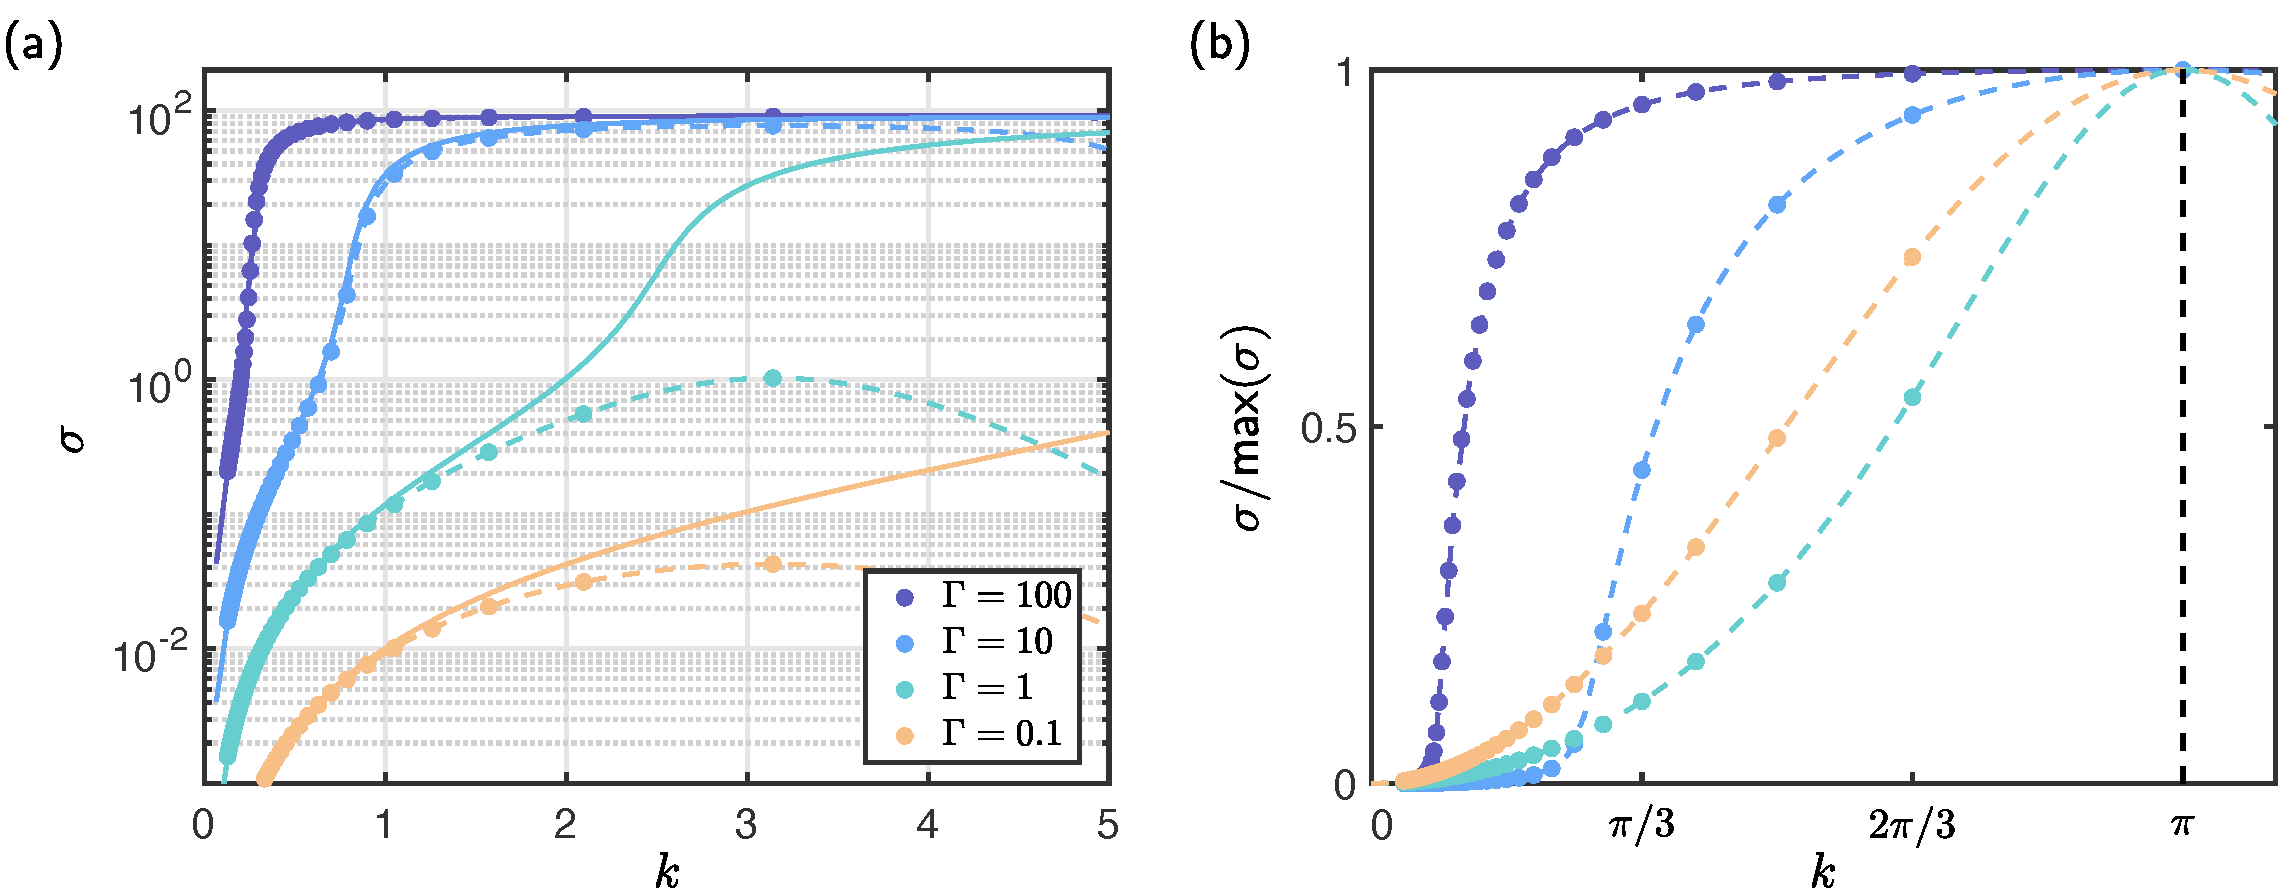
\includegraphics[width = 0.95\textwidth]{growth_rate.pdf}
\caption{Linear growth rate of periodic perturbations to an equilibrium in multi-body bendotaxis. (a) Plot of $\sigma= \sigma_{+}^{\text{cts}}(k)$ (solid curves) and $\sigma = \sigma_{+}(k)$ (dashed curves) the positive solutions of equations~\eqref{E:LSA:Continuum:DispersionRelation} and~\eqref{E:LSA:Discrete:Dispersion} with $k = 2\pi/N_p$, respectively. Note that for the continuous problem, the solid curves are simply rescaled versions of the same curve because the dispersion relation~\eqref{E:LSA:Continuum:DispersionRelation} can be rescaled to remove explicit $\Gamma$ dependence (see main text).  Markers ($\circ$) indicate discrete growth rates for perturbations with integer valued wavelengths $N_p$. Here, $V$ = 0.3, $\xbar_0 = 0.5$ and four different values of $\Gamma$ are shown (colours) as indicated by the legend in (b). The curves $\sigma_+^{\text{cts}}$ and $\sigma_+$ are indistinguishable for $\Gamma = 100$. (b) Plot of the growth rates $\sigma = \sigma_{+}(k)$ (dashed curves) for the discrete problem, and its value at integer valued wavelengths ($\circ$) normalized by their maxima $\max(\sigma)=\sigma_{+}(\pi)$.  The black dashed line indicates $k = \pi$, the wavenumber at which each of the discrete curves in (a) attains its maximum.}\label{fig:LSA:GrowthRateComparison}
\end{figure}

We denote by $\xbar$ and $\theta$ the continuous forms of $\xbar_j$ and $ \theta_{j+1/2}$, respectively. Applying the mapping~\eqref{E:LSA:Continuum:ContinuumMapping} to the governing ODEs~\eqref{E:Model:DAEs:TorqueBal} and~\eqref{E:Model:DAEs:Kinematic} gives the PDE system:
\begin{equation}\label{E:LSA:Continuum:TorqueBalancePDE}
-C_p\ddp{\theta}{t} + |\Gamma|\ddp{}{z}\left(\viscdamp\ddp{^2 \theta}{z \partial t}\right) = \theta - \frac{\Gamma}{2}\ddp{}{z}\left(\frac{2\ell I_2}{I_0h^+ h^-}\ddp{\theta}{z} + \frac{(\xbar - \ell)^2 }{h^-} - \frac{(\xbar + \ell)^2 }{h^+}\right),
\end{equation}
\begin{multline}\label{E:LSA:Continuum:KinematicPDE}
2\ddp{\xbar}{t} + \frac{1}{2} \left[\frac{\ell^2 + 2\ell \xbar}{h^+} + \frac{\ell^2 - 2\ell \xbar}{h^-} -  \frac{I^2 - \xbar^2 I^0}{I^0} \left(\frac{1}{h^+} + \frac{1}{h^-}\right)\right]\ddp{^2\theta}{z \partial t} =\\
-\frac{2\ell\sgn(\Gamma)}{3I^0 h^+ h^-} \left(\frac{1}{h^+} + \frac{1}{h^-}\right)\ddp{\theta}{z},
\end{multline}
where
\begin{equation}\label{E:LSA:Continuum:Relationships1}
\ell = \frac{V}{2} \left(1 + \xbar\ddp{\theta}{z}\right)^{-1},\quad h^{\pm} = 1 + (\bar{x}\pm \ell)\ddp{\theta}{z}, \quad I^n = \int_{\xbar - \ell}^{\xbar+\ell} x^n\left(1 + x \ddp{\theta}{z}\right)^{-3} ~\mathrm{d}x.
\end{equation}

The linear stability of the equilibrium ($\theta = 0, \xbar = \xbar_0$) is probed by considering a perturbation of the form
\begin{equation}\label{E:LSA:Continuum:Perturbation}
\theta = \delta \Theta,\quad \xbar = \bar{x}_0 + \delta X,
\end{equation}
where $\delta \ll 1$. Inserting~\eqref{E:LSA:Continuum:Perturbation}  into equations~\eqref{E:LSA:Continuum:TorqueBalancePDE}--\eqref{E:LSA:Continuum:KinematicPDE} and linearizing gives
\begin{align}
- C_p\ddp{\Theta}{t}+ |\Gamma|V^3\left(\frac{V^2}{240} + \frac{\bar{x}_0^2}{4}\right) \frac{\partial^3 \Theta}{\partial z^2 \partial t} &= \Theta - \Gamma V \left[\frac{\partial X}{\partial z} - \left(\frac{V^2}{12} + 2  \bar{x}_0^2 \right)\frac{\partial^2 \Theta}{\partial z^2}\right],\label{E:LSA:Continuum:LinearisedPDEs1}\\
2\frac{\partial X}{\partial t} +\frac{V^2}{6} \frac{\partial^2 \Theta}{\partial z \partial t} &= -\frac{2\sgn(\Gamma)}{3} \frac{\partial \Theta}{\partial z}.\label{E:LSA:Continuum:LinearisedPDEs2}
\end{align}
We can eliminate $X$ from~\eqref{E:LSA:Continuum:LinearisedPDEs1} and~\eqref{E:LSA:Continuum:LinearisedPDEs2} to give a single PDE in $\Theta$:
\begin{equation}\label{E:LSA:Continuum:SinglePDE}
- C_p\ddp{^2\Theta}{t^2}+ |\Gamma|A\frac{\partial^4 \Theta}{\partial z^2 \partial t^2} = \ddp{\Theta}{t} +  \frac{|\Gamma| V}{3}\ddp{^2 \Theta}{z^2} +\Gamma B\frac{\partial^3 \Theta}{\partial z^2\partial t}
\end{equation}
where
\begin{equation}
A = V^3\left(\frac{V^2}{240} + \frac{\bar{x}_0^2}{4}\right), \quad B = V\left(\frac{V^2}{6} + 2  \bar{x}_0^2 \right).
\end{equation}

The growth rate $\sigma$ of periodic perturbations with wavenumber $k$ (i.e. perturbations of the form $\Theta = \exp(ikz + \sigma t)$) satisfies the dispersion relation
\begin{equation}\label{E:LSA:Continuum:DispersionRelation}
\left(C_p + |\Gamma| A k^2\right)\sigma^2 + \left(1 - \Gamma B k^2\right) \sigma - \frac{|\Gamma| V}{3}k^2 = 0.
\end{equation}
This quadratic equation has two real roots for any parameter values (the discriminant of~\eqref{E:LSA:Continuum:DispersionRelation} is positive, because the product of the constant and quadratic coefficients is negative). In particular, one of these roots is positive and the other negative, so the system is unstable to perturbations of any wavenumber, and for any value of $\Gamma$. This is in contrast to some other studies of dynamic elasto-capillary aggregation in which equilibria are unstable only for sufficiently large wavenumbers and sufficiently strong surface tension~\citep{Singh2014JFM, Hadjittofis2016JFM}. It is straight-forward to show that the positive branch, denoted $\sigma_+^{\text{cts}}$, is increasing in $k$: the fastest growing instability in this continuous problem is that with the largest possible wavenumber, or smallest possible wavelength (see Figure~\ref{fig:LSA:GrowthRateComparison}). However, we expect that the continuum approximation breaks down for large wavenumber (short wavelength) perturbations, whose linear stability is therefore explored by considering the discrete equations in the next subsection.

Before moving on to this discrete analysis, we note that the dimensionless surface tension $\Gamma$ only enters~\eqref{E:LSA:Continuum:DispersionRelation} via the product $\Gamma k^2$ (for the wetting case of interest). The growth rate $\sigma$ can therefore be expressed as $\sigma(k; \Gamma) = \hat{\sigma}(\hat{k}  = \Gamma^{1/2}k)$ where $\hat{\sigma}(\hat{k})$ satisfies
\begin{equation}\label{E:LSA:Continuum:DispersionRelationRescaled}
\left(C_p +A\hat{k}^2\right)\hat{\sigma}^2 + \left(1 - B\hat{k}^2\right) \hat{\sigma} - \frac{V}{3}\hat{k}^2 = 0.
\end{equation}
This means that solid lines in Figure~\ref{fig:LSA:GrowthRateComparison}(a) showing $\sigma_+^{\text{cts}}(k; \Gamma)$ for $\Gamma = 0.1,~1,~10,~100$ are simply rescaled versions of one another, with larger values of $\Gamma$ having faster growth rates for perturbations of the same wavenumber.

\subsection{Discrete analysis}
The stability of the equilibrium state~\eqref{E:LSA:Intro:InitialCondition} is analysed by considering a periodic perturbation to equations~\eqref{E:Model:DAEs:TorqueBal} and~\eqref{E:Model:DAEs:Kinematic} of the form
\begin{equation} \label{E:LSA:Discrete:Perturbation}
\xbar_j = \xbar_0 + \delta A\exp \left[2\pi i\left(\frac{j}{N_p}-\frac{1}{4}\right)+ \sigma t\right],\quad  \theta_{j+1/2} = \delta \exp \left(\frac{2\pi i j}{N_p} +\sigma t\right),
 \end{equation}
where $A = \mathcal{O}(1)$ is the (real) relative amplitude of the perturbation in drop positions and $N_p$ its wavelength (these perturbations are analogous to continuous perturbations with wavenumber $k_p = 2\pi/N_p$). (That $\xbar_j$ must be one quarter of a period out of phase with $\theta_{j\pm1/2}$ can be understood from the kinematic condition~\eqref{E:Model:DAEs:Kinematic}. The coupling between changes in deflection angles and mean-meniscus position motion enters only through the difference in angles $\dthetaj = \theta_{j+1/2} - \theta_{j-1/2}$. Drop motion must be out of phase with   the tapering angle $\dthetaj$ as squeezing the drop -- i.e. reducing $\dthetaj$ -- increases $\xbar_j$ and vice versa, and therefore $\pi/2$ out of phase with each deflection angle.)

Inserting~\eqref{E:LSA:Discrete:Perturbation} into the model equations~\eqref{E:Model:DAEs:TorqueBal} and~\eqref{E:Model:DAEs:Kinematic} and linearizing gives the dispersion relation
\begin{multline}\label{E:LSA:Discrete:Dispersion}
\left\{C_p+ |\Gamma|V^3\left(\frac{V^2}{240} + \frac{\bar{x}_0^2}{4}\right)\left[2 - 2\cos\left(\frac{2\pi}{N_p}\right)\right]\right\}\sigma^2 +\\ \left\{1 - \Gamma V\left[\frac{V^2}{3} \sin^2 \left(\frac{\pi}{N_p}\right) +\left( \frac{V^2}{12}+ 2\xbar_0^2\right)\left(2 - 2\cos\left(\frac{2\pi}{N_p}\right)\right)\right]\right\}\sigma-\\ \frac{4V|\Gamma|}{3}\sin^2\left(\frac{\pi}{N_p}\right) = 0,
\end{multline}
as well as the amplitude
\begin{equation}\label{E:LSA:Discrete:Amplitude}
A = \frac{V^2 \sigma + 4 \sgn(\Gamma)}{\sigma}\sin\left(\frac{\pi}{N_p}\right).
\end{equation}
Note that the dispersion relation~\eqref{E:LSA:Continuum:DispersionRelation} is recovered from~\eqref{E:LSA:Discrete:Dispersion} in the limit $N_p \gg 1$. Unlike the continuous case, however, the parameter $\Gamma$ cannot be scaled out of the dispersion relation~\eqref{E:LSA:Discrete:Dispersion} for $N_p = \mathcal{O}(1)$.

Equation~\eqref{E:LSA:Discrete:Dispersion} has one positive (denoted $\sigma_+$) and one negative real root, as in the continuous case, thus confirming that the undeformed equilibrium~\eqref{E:LSA:Intro:InitialCondition} is unstable to perturbations of any wavenumber. In contrast to the continuous case, however, these roots are not monotonic as functions of $N_p$ (equation~\eqref{E:LSA:Discrete:Dispersion} is $2\pi$ periodic in $k_p=2\pi/N_p$) --  $\sigma_+$ has maxima at odd integer multiples of $\pi$ (see Figure~\ref{fig:LSA:GrowthRateComparison}(a)). The smallest wavenumber $k_p$ which is a maximum is $k_p = \pi$, corresponding to $N_p = 2$. $N_p = 2$ is also a lower bound on the wavelength of perturbations (which must be integer valued), i.e. $k_p = \pi$ is an upper bound on wavenumbers. As $\sigma_+$ is increasing for $0 < k < \pi$, we conclude that the instability with $N_p = 2$ is the fastest growing.

\subsection{Discussion}\label{S:LSA:Discussion}
Both the continuous and discrete linear stability analyses show that perturbations to the equilibrium state~\eqref{E:LSA:Intro:InitialCondition} of any wavelength are unstable. Thus we have answered the question posed at the start of the section: the numerical solutions presented in \S\ref{S:Numerics} do not decay to the equilibrium close to which they started because this equilibrium is unstable, which would have been the case for any choice of droplet volume and position. We have also seen that the pairwise mode, $N_p = 2$, is always the fastest growing mode in the linear analyses. It might be expected, therefore, that a random initial condition (as in \S\ref{S:Numerics}) would always select a pairwise mode; however this is not the case since clusters of various sizes, which correspond to different wavelength modes, can be observed in the numerical solutions even at early times when the linear analysis holds.

We can gain insight into the appearance of other modes by comparing the \emph{relative} size of the growth rates of different wavenumber perturbations. Figure~\ref{fig:LSA:GrowthRateComparison}(b) displays the (discrete) growth rates, normalized by their maxima (attained at $N_p = 2$). Those normalized growth rates which are shallow near $k = \pi$ (e.g. the purple $\Gamma  = 100$ curve in Figure~\ref{fig:LSA:GrowthRateComparison}(b)) will have similar growth rates for many of the largest possible wavenumbers; the modes corresponding to these wavenumbers will grow comparably during the period in which the linear analysis is valid. This argument agrees qualitatively with observations: growth rates are shallower near $k = \pi$ in Figure~\ref{fig:LSA:GrowthRateComparison}(b) for larger $\Gamma$, and a greater range of cluster sizes is observed for larger $\Gamma$ in the numerical solutions in \S\ref{S:Numerics} (Figure~\ref{fig:Numerics:ClusterSizes}).

Quantitative predictions about the range of cluster sizes observed can be made when $\Gamma$ is large and the continuous analysis applies (note that the discrete and continuous growth rates are indistinguishable when $\Gamma \gg 1$, see Figure~\ref{fig:LSA:GrowthRateComparison}(a)). As described in \S\ref{S:LSA:Continuum}, in this case, $\Gamma$ can be scaled out of the problem by setting $\hat{k} = \Gamma^{1/2}k$. This implicitly identifies a lengthscale in the $z$-direction which scales with $\Gamma^{1/2}$. We might therefore expect that the range of similar growth rates, and hence range of early time cluster sizes in numerical solutions of the full problem with random initial conditions, should scale with $\Gamma^{1/2}$.

In fact, we observe a stronger result: numerical solutions of the full problem with random initial conditions have a range of cluster sizes that scales with $\Gamma^{1/2}$ even at late times, as shown in Figure~\ref{fig:LSA:Clustering:ClusterSizes}. The other clear trend in this figure is that the system almost always selects the pairwise mode for $\Gamma < 1$ (i.e. the linear stability prediction is followed here). The following section is devoted to explaining the mechanisms behind these observations.

\begin{figure}[t]
\centering
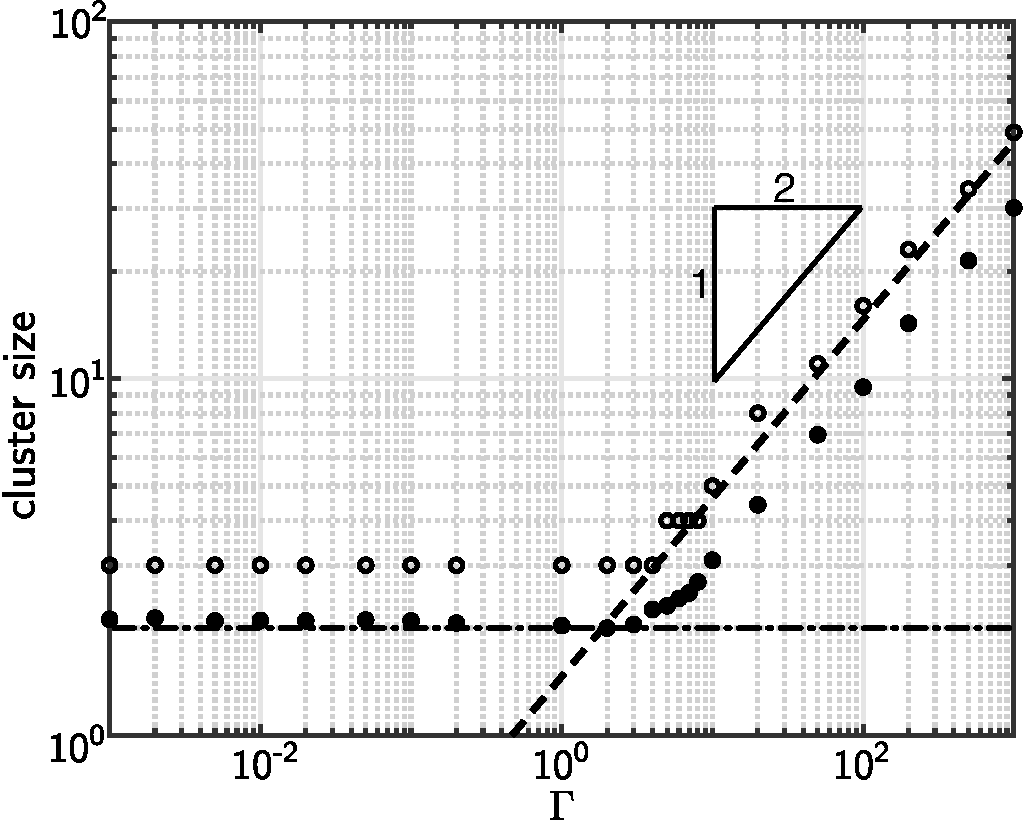
\includegraphics[scale=0.5]{cluster_size_vs_Gamma}
\caption{Clustering behaviour of multibody bendotaxis. Open circles indicate maximum cluster size (and hence range of cluster sizes) and filled circles indicate average cluster size in an ensemble numerical solutions of the full problem~\eqref{E:NumSols:MDE:MatrixDifferentialEquation} with random initial conditions~\eqref{E:NumSols:MDE:IC} (sampled from a uniform random distribution on $\left[-1,1\right]$, and $\epsilon = 10^{-3}$). Cluster sizes are evaluated when every drop is at least 90$\%$ of the way along the channel (towards the base or the free end). In these solutions, $V = 0.3$ and $\xbar_0 = 0.5$ and $N = 199$ channels are used. Each data point is obtained by averaging over 10 solutions with a unique initial condition. The dashed line indicates the asymptotic prediction~\eqref{E:ClusterSizes:LargeGamma:Scaling} for strong surface tension, $\Gamma \gg 1$ and the dot-dashed corresponds to the pairwise mode predicted analytically in \S\ref{S:ClusterAnalysis:SmallGamma}.  }\label{fig:LSA:Clustering:ClusterSizes}
\end{figure}

\section{Analysis of cluster sizes}\label{S:ClusterAnalysis}
In this section, we explain quantitatively the salient trends in the mean and maximum cluster sizes shown in Figure~\ref{fig:LSA:Clustering:ClusterSizes}: in particular, we seek to explain the $\Gamma^{1/2}$ scaling for  $\Gamma \gg 1$, and the selection of a pairwise mode for $\Gamma \ll 1$.

\subsection{Strong surface tension, $\Gamma \gg 1$}

\begin{figure}[t]
\centering
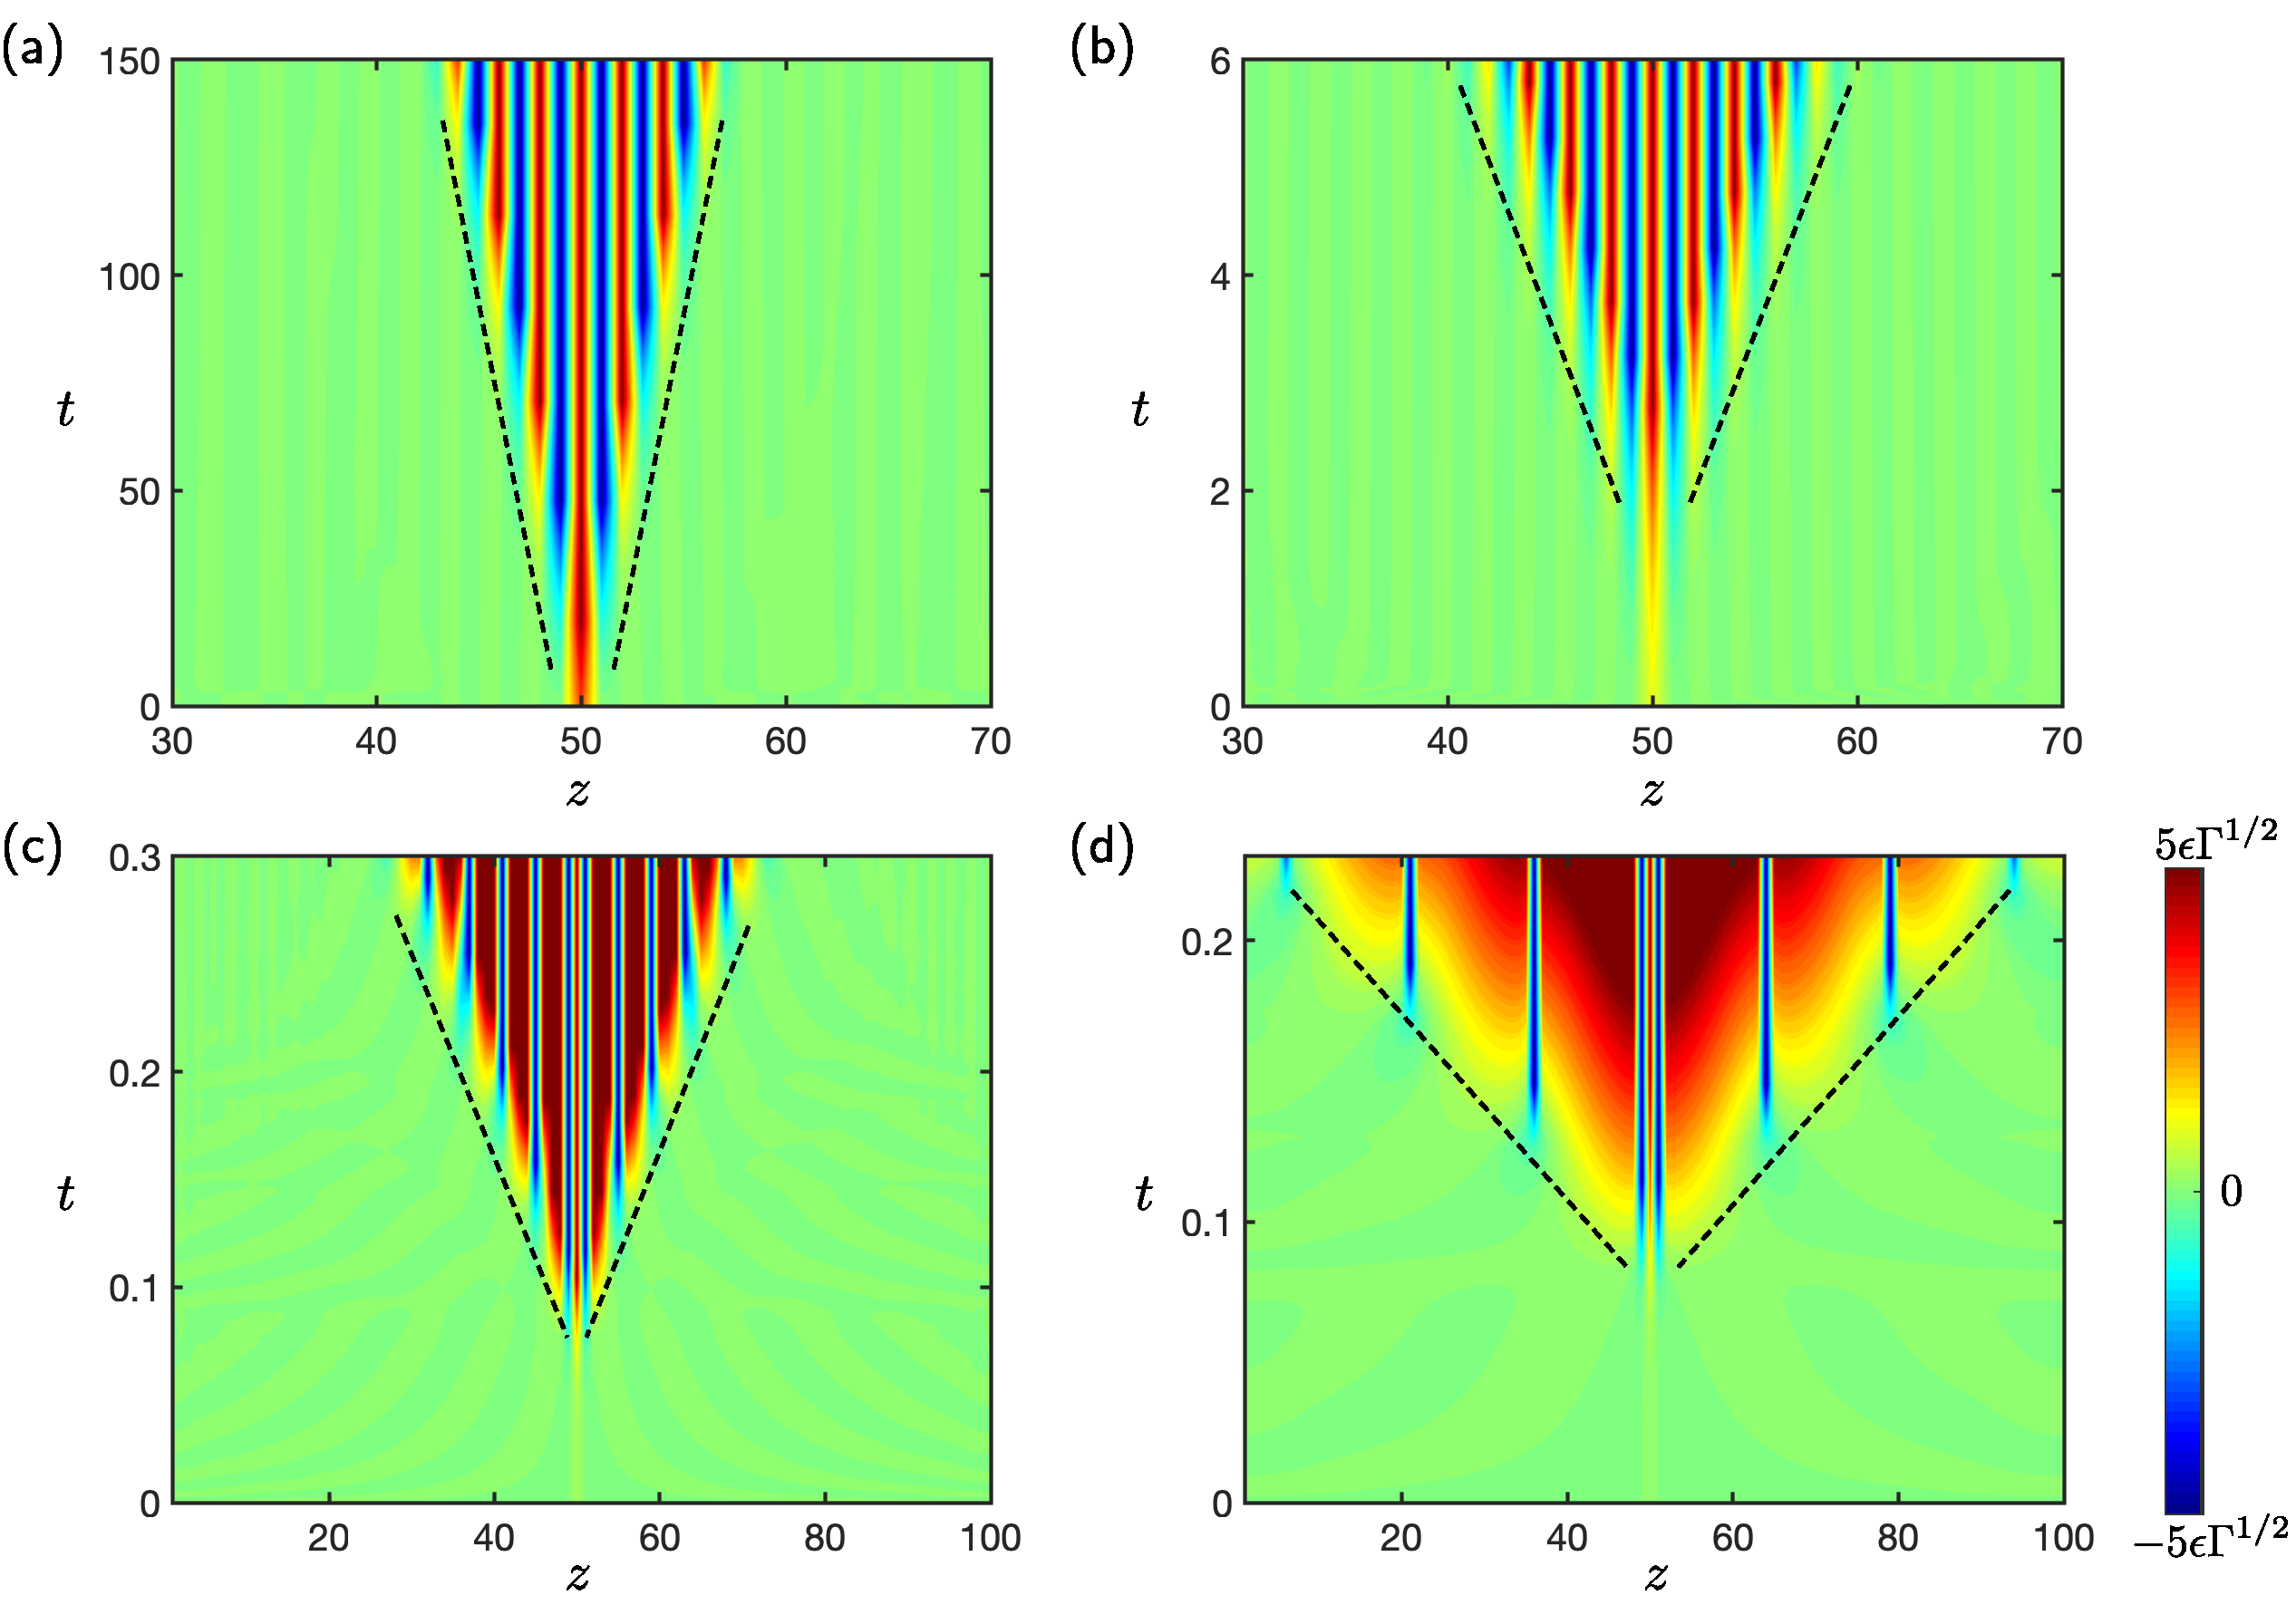
\includegraphics[width = 0.95\textwidth]{Wedges}
\caption{Spatiotemporal plots of the displacement $\xbar_j - \bar{x}_0$ from a local perturbation of the form $\xbar_j^0 =0.5 +\epsilon \delta_{j,50}, \theta_{j+1/2}^0 = 0$ ($\delta_{j,k}$ is the Kronecker delta) obtained numerically by solving equation~\eqref{E:NumSols:MDE:MatrixDifferentialEquation} with $N = 100$ channels and equal drop volumes $V_j = 0.3$, and $\epsilon = 10^{-3}$. Results with four different values of $\Gamma$ are shown as follows: (a) $\Gamma = 0.1$, (b) $\Gamma = 1$,  (c) $\Gamma = 10$, (d) $\Gamma = 100$. The colourbar in (d) applies to each of the plots with the appropriate value of $\Gamma$. Observe that the propagation of the disturbance away from its initial position appears to be confined to a wedge bounded by two approximately straight lines (dashed lines, acting as a guide for the eyes).}\label{fig:ClusterSizes:Wedges}
\end{figure}

The mean and maximum cluster sizes for $\Gamma \gg 1$ (Figure~\ref{fig:LSA:Clustering:ClusterSizes}) are reminiscient of those reported by~\cite{Singh2014JFM} who observed a similar scaling in their spring-block model of elasto-capillary aggregation. They were able to predict the prefactor of this scaling after noticing that the disturbance propagating from a localised perturbation (that is, a perturbation in a single channel) grows only within a `wedge' bounded by two straight lines in spatiotemporal plots. Our torsion spring model appears to behave similarly (see Figure~\ref{fig:ClusterSizes:Wedges}). Motivated by these similarities, we investigate whether the mechanism responsible for selecting cluster sizes in the case of strong surface tension identified by Singh et al. (described in the next section) is also the mechanism selecting cluster sizes in the limit $\Gamma \gg 1$ in our torsion spring system.

\subsubsection{Qualitative discussion of \cite{Singh2014JFM}}
Singh et al.~observed fronts propagating at a constant speed from a localised initial condition, therefore defining a wedge in spatiotemporal plots inside which solutions grew in time, and outside which they decayed in time. They noticed that monodisperse clusters formed in the vicinity of this wedge, whose (uniform) size scaled with the square root of dimensionless surface tension as predicted by their linear analysis of the same problem. Further, these clusters were found to persist -- the late time cluster distribution is also monodisperse, with this same cluster size. They explained that the cluster size must be `frozen in' near the leading edge of the wedge and that, as the displacements are small in the vicinity of the wedge, the linearised analysis can predict this cluster size.

By solving the linearized equations explicitly in both the discrete and continuous cases, they obtained predictions of the cluster size; these predictions were identical for strong surface tension, indicating that the long wavelength structures formed in this case are described well by the continuous model.

Their linearised PDE in the perturbation to channel widths, $H(y,t)$ is
\begin{equation}\label{E:Clusters:Singh:PDE}
\ddp{^3 H}{y^2 \partial t} - 2\ddp{^2 H}{z^2} = 2K H,
\end{equation}
where $K^{-1}$ is the dimensionless surface tension of their system. To solve equation~\eqref{E:Clusters:Singh:PDE} Singh et al. took a Fourier transform in space, solved the resulting equation and expressed the solution in physical space as an inverse Fourier integral
\begin{equation}
H(y,t) = \frac{1}{2\pi}\int_{-\infty}^{\infty} \hat{H}_0(s)\exp\left(isy - \frac{2Kt}{s^2}\right)~\mathrm{d}s,
\end{equation}
where $\hat{H}_0(s)$ is the Fourier transform of their initial condition. To understand the behaviour of the integral, they considered its behaviour along rays -- lines of the form $y = ct$ -- at late times, by applying the method of steepest descent. In particular, they found that
\begin{equation}\label{E:Clusters:Singh:Solution}
H(y,t) \propto \frac{2^{5/6}K^{1/6}t^{1/6}}{3^{1/2}\pi^{1/2}y^{2/3}}\exp\left[2t\left(1 - \frac{3K^1/3}{2^{7/3}}\frac{y^{2/3}}{t^{2/3}}\right)\right]\cos \left[ \frac{3^{3/2}}{2^{4/3}}(Ky^2 t)^{1/3}\right]
\end{equation}
along rays, as $t \to \infty$. The solution~\eqref{E:Clusters:Singh:Solution} only grows along rays which are travelling sufficiently slowly, i.e. for $c < c_{\max} = 2^{7/2}K^{-1/2}/3^{3/2}$ (for $c > c_{\max}$, the solution~\eqref{E:Clusters:Singh:Solution} decays exponentially in time). Their wedge shape is thus given by $z = c_{\max} t$. As well as this exponential envelope, the solution~\eqref{E:Clusters:Singh:Solution} has an oscillatory term; the monodisperse cluster size prediction was then seen to correspond to the speed of propagation of the front $c_{\max}$ divided by the frequency of oscillations along it, $\omega_{\max} = 3^{3/2}/\pi$ and thus scaling with $K^{-1/2}$.

This prediction from analysing a localised perturbation also accurately predicted the maximum cluster size in numerical solutions of the full system with random initial conditions. They rationalized that a random initial condition contains many localised perturbations, from each of which a front propagates and (provided it does not interact with other fronts) locks in the monodisperse cluster sizes discussed above. When fronts interact, they act destructively and form clusters whose size is below this monodisperse size. Over a large number of channels, these effects give a distribution of cluster sizes bounded by the monodisperse cluster size.

We hypothesize that the `locking-in' of clusters around fronts associated with localised perturbations may also be responsible for the appearance of the $\Gamma^{1/2}$ scaling in our maximum cluster sizes. In the next section we discuss how to solve the linearised PDE system (expected to be relevant for the long wavelength structures) to obtain the pre-factor in this scaling.

 \subsubsection{Solving the linearized PDEs}
 \begin{figure}[t]
\centering
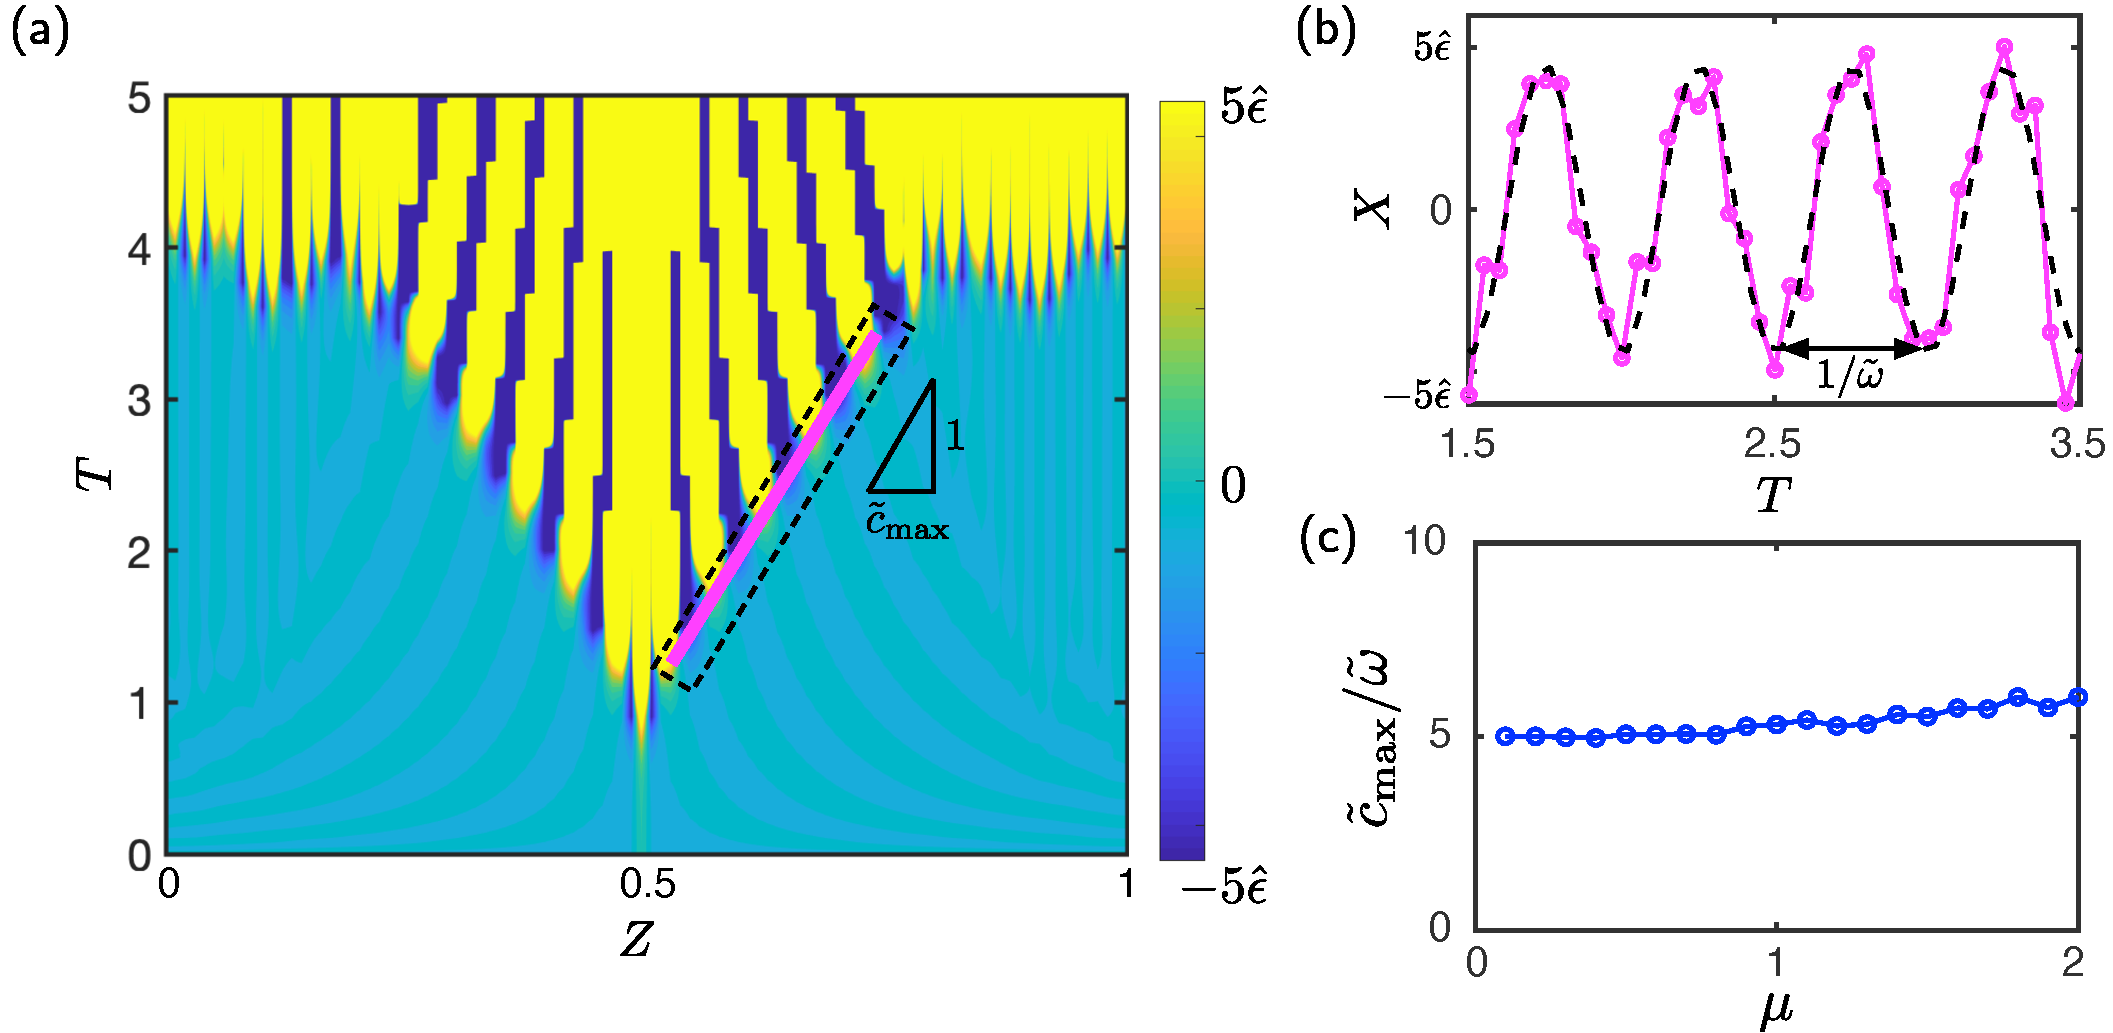
\includegraphics[width = 0.95\textwidth]{Redicretised_wedge_new}
\caption{(a) Spatiotemporal plot of $X(Z,T)$, obtained numerically by solving equations~\eqref{E:ClusterSizes:LargeGamma:ScaledPDE1} and \eqref{E:ClusterSizes:LargeGamma:ScaledPDE2} with initial condition~\eqref{E:ClusterSizes:LargeGamma:ICscaled2} corresponding to a localised perturbation. Here, the perturbation has magnitude $\epsilon = 10^{-3}$, $\mu =V/\bar{x}_0= 0.6$ and the perturbation is located at $Z_0 = 0.55$.  The magenta line (fitted by eye) indicates the wedge inside which the perturbation grows. Note that far away from the wavefront inside the wedge (where the pattern is coarse), we expect large deformations and therefore the linearized analysis does not apply. The disturbance is only confined to a wedge for  $T \lesssim 4$ at which point noise growing in the far field has magnitude comparable to that along the wavefront. (b) plot of $\chi(Z = Z_0 + \tilde{c}_{\max},T)$  (i.e. the cross section of $\chi$ taken along the magenta line in (a), magenta curve) and a single mode Fourier fit with frequency $\tilde{\omega}$ to this (black dashed curve). (c) Plot of scaled cluster size $\tilde{c}_{\max}/\tilde{\omega}$ for $\mu$ in the  range of physically realistic values. Each point is obtained by solving numerically the PDE system~\eqref{E:ClusterSizes:LargeGamma:ScaledPDE1}--\eqref{E:ClusterSizes:LargeGamma:ScaledPDE2}, finding $\tilde{c}_{\max}$ by fitting the line $Z \propto \tilde{c}_{\max} T$ by eye, and obtaining $\tilde{\omega}$ by fitting a single mode Fourier series to the solution along this line. }\label{fig:ClusterSizes:LargeGamma:RediscretisedWegde}
\end{figure}

Recall that the system of PDEs for wetting drops, obtained by considering $\theta = \varepsilon \Theta, \xbar = \xbar_0 +  \varepsilon X$, and linearizing in $ \varepsilon \ll 1$:
\begin{align}
- C_p\ddp{\Theta}{t}+ \Gamma V^3\left(\frac{V^2}{240} + \frac{\bar{x}_0^2}{4}\right) \frac{\partial^3 \Theta}{\partial z^2 \partial t} &= \Theta - \Gamma V \left[\frac{\partial X}{\partial z} - \left(\frac{V^2}{12} + 2  \bar{x}_0^2 \right)\frac{\partial^2 \Theta}{\partial z^2}\right],\label{E:ClusterSizes:LargeGamma:LinearisedPDEs1}\\
2\frac{\partial X}{\partial t} +\frac{V^2}{6} \frac{\partial^2 \Theta}{\partial z \partial t} &= -\frac{2}{3} \frac{\partial \Theta}{\partial z}.\label{E:ClusterSizes:LargeGammaLinearisedPDEs2}
\end{align}
To analyse a localized perturbation about $z = z_0$, we consider initial conditions of the form
\begin{equation}\label{E:ClusterSizes:LargeGamma:InitialCondition}
\Theta(z, 0) = 0, \quad X(z,0) = f(z; z_0) =
\begin{cases}
1& \text{for}~|z-z_0| < 1/2,\\
0 & \text{otherwise}.
\end{cases}
\end{equation}

Note that by introducing scaled variables,
\abceqn{E:ClusterSizes:LargeGamma:ScaledVariables}{\phi = \frac{\Gamma^{1/2}\bar{x}_0}{V^{3/2}}\Theta,\quad T = \frac{1}{V^2}t,\quad Z = \frac{1}{\bar{x}_0 V^{1/2} \Gamma^{1/2}}z,}
the PDE system~\eqref{E:ClusterSizes:LargeGamma:LinearisedPDEs1}--\eqref{E:ClusterSizes:LargeGammaLinearisedPDEs2} is reduced to
\begin{align}
- \tilde{C}\ddp{\phi}{T}+ \left(\frac{\mu^2}{240} + \frac{1}{4}\right) \frac{\partial^3 \phi}{\partial Z^2 \partial T} &= \phi - \mu^2 \frac{\partial X}{\partial Z} + \left(\frac{\mu^2}{12} + 2   \right)\frac{\partial^2 \phi}{\partial Z^2},\label{E:ClusterSizes:LargeGamma:ScaledPDE1}\\
2\frac{\partial X}{\partial T} +\frac{1}{6} \frac{\partial^2 \phi}{\partial Z \partial T} &= -\frac{2}{3} \frac{\partial \phi}{\partial Z},\label{E:ClusterSizes:LargeGamma:ScaledPDE2}
\end{align}
where $\mu = V/\bar{x}_0$ is a geometric parameter whose value is restricted to $0 < \mu < 2$ by channel geometry, and $\tilde{C} = C_p /V^2$. Note that here we have explicitly identified the lengthscale $L_z =  \xbar_0V^{1/2}\Gamma^{1/2}$, whose scaling with $\Gamma^{1/2}$ was discussed in \S\ref{S:LSA:Discussion}. The PDE system~\eqref{E:ClusterSizes:LargeGamma:ScaledPDE1}--\eqref{E:ClusterSizes:LargeGamma:ScaledPDE2} and corresponding initial conditions
\begin{equation}\label{E:ClusterSizes:LargeGamma:ICscaled2}
\phi(Z,0) = 0, \quad  X(Z,0) = f\left(Z; Z_0 = \frac{z_0}{x_0 V^{1/2}\Gamma^{1/2}} \right) =
\begin{cases}
1& \text{for}~|Z-Z_0| < \frac{1}{2L_z},\\
0 & \text{otherwise}.
\end{cases}
\end{equation}
have no parametric dependence on $\Gamma$ except via the breadth of the perturbation, which was arbitrary prior to rescaling. In the numerical results presented here, we take $1/L_z = 10^{-3} \ll 1$ to reflect the fact that $\Gamma \gg 1$.

After taking a Fourier transform in space, the linear problem~\eqref{E:ClusterSizes:LargeGamma:ScaledPDE1}--\eqref{E:ClusterSizes:LargeGamma:ScaledPDE2} becomes
\begin{equation}\label{E:ClusterSizes:LargeGamma:ft1}
\dd{\hat{\underline{u}}}{t} =\mathbf{A}^{-1}\mathbf{B}\hat{\mathbf{u}}
\end{equation}
where $\hat{\underline{u}} = (\hat{\phi}(T;s), \hat{X}(T;s))^\intercal$ is the Fourier transform of $\underline{u} = (\phi(Z,T), X(Z,T))^\intercal$ and
\begin{equation}\label{E:ClusterSizes:LargeGamma:ftmatrices}
\mathbf{A} = \begin{bmatrix}
-\hat{C} - \left(\frac{\mu^2}{240} +\frac{1}{4}\right) s^2 & 0 \\
\frac{is}{6} & 2
\end{bmatrix}, \quad \mathbf{B}= \begin{bmatrix}
1 - \left(\frac{\mu^2}{12} +2\right) s^2 & -\mu^2 i s \\
-\frac{2is}{3} & 0
\end{bmatrix}.
\end{equation}
The problem~\eqref{E:ClusterSizes:LargeGamma:ft1}--\eqref{E:ClusterSizes:LargeGamma:ftmatrices} can be solved alongside the initial condition
\begin{equation}
\hat{\underline{u}}(0;s) = \begin{bmatrix}
0\\ \hat{f}
\end{bmatrix},
\end{equation}
thus allowing $\hat{\underline{u}}$ to be expressed as an inverse Fourier integral:
\begin{equation}\label{E:ClusterSizes:LargeGamma:ft_inverse}
\underline{u}(Z,T) = \frac{1}{2\pi}\int_{-\infty}^{\infty} \left[(\hat{\underline{u}}(0;s).\underline{v}_1) \underline{v}_1 e^{m_1(s) T }+(\hat{\underline{u}}(0;s).\underline{v}_2) \underline{v}_2 e^{m_2(s) T }\right]e^{isZ}~\mathrm{d}s
\end{equation}
where $\underline{v}_i, i = 1,2$ are orthonormal eigenvectors of $ \mathbf{A}^{-1}\mathbf{B}$, and $m_i, i = 1,2$ are the corresponding eigenvalues (these are solutions of the dispersion relation~\eqref{E:LSA:Continuum:DispersionRelation} after scaling the variables according to~\eqref{E:ClusterSizes:LargeGamma:ScaledVariables}).

The integral~\eqref{E:ClusterSizes:LargeGamma:ft_inverse} must be evaluated numerically, in general\footnote{In~\cite{Singh2014JFM}, the steepest descent calculation involves finding the saddle points of the function $\psi(s) = isc - 1/s^2$ in $\mathbb{C}$, i.e. $s = (2/c)^{1/3}(i/2 \pm \sqrt{3}/2)$. The corresponding calculation here requires locating the saddle points of $\psi(s) = isc + m_{i}(s)$, which cannot be done analytically for a general $\mu= V/\bar{x}_0$.}.  With the technology we have developed so far in this chapter, it is simpler, however, to solve the original PDE system~\eqref{E:ClusterSizes:LargeGamma:ScaledPDE1}--\eqref{E:ClusterSizes:LargeGamma:ScaledPDE2} numerically on $\left[0, N\right]$ using the method of lines with $N$ grid points; this is equivalent to solving the ODE system that is obtained by applying the scalings~\eqref{E:ClusterSizes:LargeGamma:ScaledVariables}a,b to the linearized discrete equations and normalizing channel widths to the lengthscale $L_z$ by mapping $()_{j+1} - ()_j \to [()_{j+1} - ()_j]/L_z$. (We do not discuss the numerical scheme in more detail as it is essentially the same as that described in \S\ref{S:Numerics:Details}.)

A spatiotemporal plot of the numerical solution of~\eqref{E:ClusterSizes:LargeGamma:ScaledPDE1}--\eqref{E:ClusterSizes:LargeGamma:ScaledPDE2} with initial condition~\eqref{E:ClusterSizes:LargeGamma:ICscaled2} (Figure~\ref{fig:ClusterSizes:LargeGamma:RediscretisedWegde}) shows  that the growth of the perturbation is confined to a wedge bounded by lines parallel to $Z-Z_0 = \pm \tilde{c}_{\max} T$ (the slope $\tilde{c}_{\max}$ of these lines is fitted by eye). As in~\cite{Singh2014JFM}, the solution is oscillatory at the edge of the wedge (see Figure~\ref{fig:ClusterSizes:LargeGamma:RediscretisedWegde}(b)); the frequency of oscillation along it, $\tilde{\omega}$, is determined by performing a (single term) Fourier fit in \textsc{matlab}.

Following~\cite{Singh2014JFM}, the monodisperse cluster size in this scaled problem is $\tilde{c}_{\max}/\tilde{\omega}$, corresponding to a localized perturbation cluster size (and hence a maximum cluster size with random initial conditions) of
\begin{equation}\label{E:ClusterSizes:LargeGamma:ClusterSize}
N_c = \frac{\bar{x}_0 V^{1/2}\tilde{c}_{\max}}{\tilde{\omega}}\Gamma^{1/2},
\end{equation}
after reversing the scalings in~\eqref{E:ClusterSizes:LargeGamma:ScaledVariables}.

For the particular case $\xbar_0 = 0.5$, $V = 0.3$, we find ${c}_{\max}\approx  10$ and $\omega \approx 2$ (Figure~\ref{fig:ClusterSizes:LargeGamma:RediscretisedWegde}). This predicts a maximum cluster size
\begin{equation}\label{E:ClusterSizes:LargeGamma:Scaling}
N_c \approx 1.3~\Gamma^{1/2},
\end{equation}
which shows very good agreement with maximum cluster size of numerical solutions with random initial conditions (Figure~\ref{fig:LSA:Clustering:ClusterSizes}).

Finally, we note that the ratio $\tilde{c}_{\max}/\tilde{\omega}$ is approximately independent of $\mu$ ($\tilde{c}_{\max}/\tilde{\omega} \approx 5$, see Figure~\ref{fig:ClusterSizes:LargeGamma:RediscretisedWegde}(c)); we therefore expect that cluster size statistics for values of $\xbar_0$ and $V$ different to those used in Figure~\ref{fig:LSA:Clustering:ClusterSizes} will follow the scaling
\begin{equation}
N_c \approx 5\bar{x}_0 V^{1/2} \Gamma^{1/2}
\end{equation}
for $\Gamma \gg 1$.


\subsection{Weak surface tension, $\Gamma \ll 1$}\label{S:ClusterAnalysis:SmallGamma}
%This is the most unstable mode in the linear stability analysis, regardless of the value of $\Gamma$, is a pairwise one. We have seen that, for $\Gamma \gg 1$, a range of cluster sizes, rather than just this pairwise mode, are observed in numerical solutions with random initial conditions by analysing the wedge like structure associated with a localized perturbation. Figure~\ref{fig:ClusterSizes:Wedges} suggests that for $\Gamma \ll 1$, disturbances from a localized perturbation also propagate into a wedge, so we might expect to range of cluster sizes formed from a random perturbation, in this limit, but this clearly does not happen (~\ref{fig:ClusterSizes:Wedges}).In this section, we analyse the governing equations in the limit $\Gamma \ll 1$ to explain quantitatively why the system always selects the pairwise mode.

In this section, we solve analytically the discrete governing equations (equations \eqref{E:Model:DAEs:TorqueBal} and~\eqref{E:Model:DAEs:Kinematic}) with a generalized initial condition
\begin{equation}\label{E:ClusterSizes:SmallGamma:IC}
\underline{x}(0) = \left(\theta_{3/2}^0, \dots, \theta_{N+1/2}^0,\xbar_1^0,\dots, \xbar_N^0\right)^\intercal = \underline{x}^0,
\end{equation}
and equal volume drops, $V_j = V$, in the limit $\Gamma \ll 1$.

As mentioned earlier in \S\ref{S:SingleChannel:FlexibleComparison} for a single channel,  the discrete equations decouple onto two distinct time scales in the limit $|\Gamma| \to 0$ (see Appendix~\ref{Appendix:SmallGammaAnalysis} for full details). With multiple channels, rather than a single channel, the behaviour is subtly different: on a fast ($\mathcal{O}(|\Gamma|)$) time scale, the deflection angles move towards a quasi-equilibrium set by the difference in capillary forces applied by the adjacent droplets (rather than by the capillary force from a single droplet).  The droplets move towards the end of their channels on a long ($\mathcal{O}(|\Gamma|^{-1})$) timescale; this motion is governed by the ODE
\begin{equation}\label{E:ClusterSizes:SmallGamma:LongTimescaleEquation}
\dd{\underline{\xbar}}{t} = -\frac{|\Gamma|V}{3}D^2 \underline{\xbar},
\end{equation}
where $D^2$ is the periodic form of the discrete Laplacian matrix
\begin{equation}\label{E:ClusterSizes:SmallGamma:LongTimescaleMatrix}
D^2=  \begin{bmatrix}
-2 & 1   & & & 1 \\
1 & -2 & 1  \\
 & 1 & \ddots & \ddots \\
& & \ddots & \ddots & 1 \\
1& & &1&- 2
\end{bmatrix},
\end{equation}
where empty entries indicate zeros.

The solution to~\eqref{E:ClusterSizes:SmallGamma:LongTimescaleEquation} with initial condition $\underline{\xbar}^0 = \left(\xbar_1^0,\dots, \xbar_N^0\right)^\intercal$  is
\begin{equation}\label{E:ClusterSizes:SmallGamma:Solution}
\underline{\xbar} = \sum_{p=1}^{N} (\underline{\xbar}^0.\underline{v}_p)\underline{v}_p\exp\left(-\frac{|\Gamma|V}{3}\lambda_p t\right),
\end{equation}
where the $\lambda_p,~ p = 1,\dots, N$ are the eigenvalues of $D^2$, i.e.
\begin{equation}\label{E:ClusterSizes:SmallGamma:Eigenvalues}
\lambda_p =\left\{
 \begin{array}{ll}
-4\sin^2\left(\frac{\pi(p-1)}{2N}\right) & p \text{~odd,}\\
-4\sin^2\left(\frac{\pi p}{2N} \right) & p\text{~even,}\\
 \end{array}\right.
\end{equation}
and $\underline{v}_p$ are the corresponding eigenvectors whose $q^{\th}$ component is
\begin{equation}\label{E:ClusterSizes:SmallGamma:Eigenvectors}
\underline{v}_{p,q} =N^{-1/2} \times\left\{
 \begin{array}{ll}
1&  \text{if}~p = 1,\\
 (-1)^q   & \text{if}~p = N ~ \text{and} ~ N ~\text{is even,}\\
\sqrt{2}\sin \left(\frac{\pi(q-1/2)p}{N}\right) & \text{otherwise, with}~p ~ \text{even,} \\
  \sqrt{2}\cos \left(\frac{\pi(q-1/2)(p-1)}{N}\right) & \text{otherwise, with}~p ~ \text{odd.} \\
  \end{array}\right.
\end{equation}
The solution~\eqref{E:ClusterSizes:SmallGamma:Solution} shows good agreement with numerical solutions of the full problem (see Appendix~\ref{Appendix:SmallGammaAnalysis}).

Note that all eigenvalues are negative, and the largest in absolute value is $\lambda_N =-4$. When $N$ is even, the corresponding eigenvector is $\underline{v}_N = N^{1/2}\left(1,-1,1,-1,\dots,-1\right)^\intercal$, corresponding to a pairwise mode in which droplets move in opposite directions to their neighbours. For odd values of $N$, the eigenvector associated with $\lambda_N$ also has entries with equal magnitude whose sign alternates, but the first and final entries have the same sign and value. This means that when $N$ is odd, the system selects a pairwise mode everywhere except for at the periodic boundary, across which the drops move in the same direction (towards the free end), giving a cluster of three plates; this explains why the maximum cluster size in numerical solutions is $N_c = 3$ even as $\Gamma \to 0$ (Figure~\ref{fig:LSA:Clustering:ClusterSizes}).

We note finally that, if we consider initial conditions corresponding to a localised perturbation (i.e. $\underline{\xbar}^0  = (\xbar_0, \dots, \xbar_0, \xbar_0 + \epsilon, \xbar_0, \dots, \xbar_0)^\intercal$) as in the previous section, the solution~\eqref{E:ClusterSizes:SmallGamma:Solution} reduces to
\begin{equation}\label{E:clusterSizes:SmallGamma:SolutionLocalPert}
\bar{x}_{j} = \bar{x}_0 + \frac{\epsilon\Gamma}{N}\left\{1 + 2\sum_{p = 1}^{\floor{N/2}} \cos\left[\frac{2\pi p (k-j)}{N}\right]\exp\left[\frac{4}{3V}\sin^2\left(\frac{p\pi}{N}\right)|\Gamma|t\right]\right\},
\end{equation}
where $k$ is the index of the disturbance. This solution grows in time everywhere, rather than only within a wedge, as was the case for $\Gamma \gg 1$. (Note that equation~\eqref{E:ClusterSizes:SmallGamma:LongTimescaleEquation} is the discretization of the backwards heat equation, which is famously ill-posed and characteristically transmits information infinitely quickly). Whilst it appears from Figure~\ref{fig:ClusterSizes:Wedges}(a) that the growth of a localized perturbation for $\Gamma = 0.1$ is confined to a wedge, the solution~\eqref{E:clusterSizes:SmallGamma:SolutionLocalPert} shows that this is not the case: the displacement is constant along lines approximately given by $z = c \exp(t^2)$.

\section{Droplet removal in multi-body bendotaxis}\label{S:Discussion}
\begin{figure}[t]
\centering
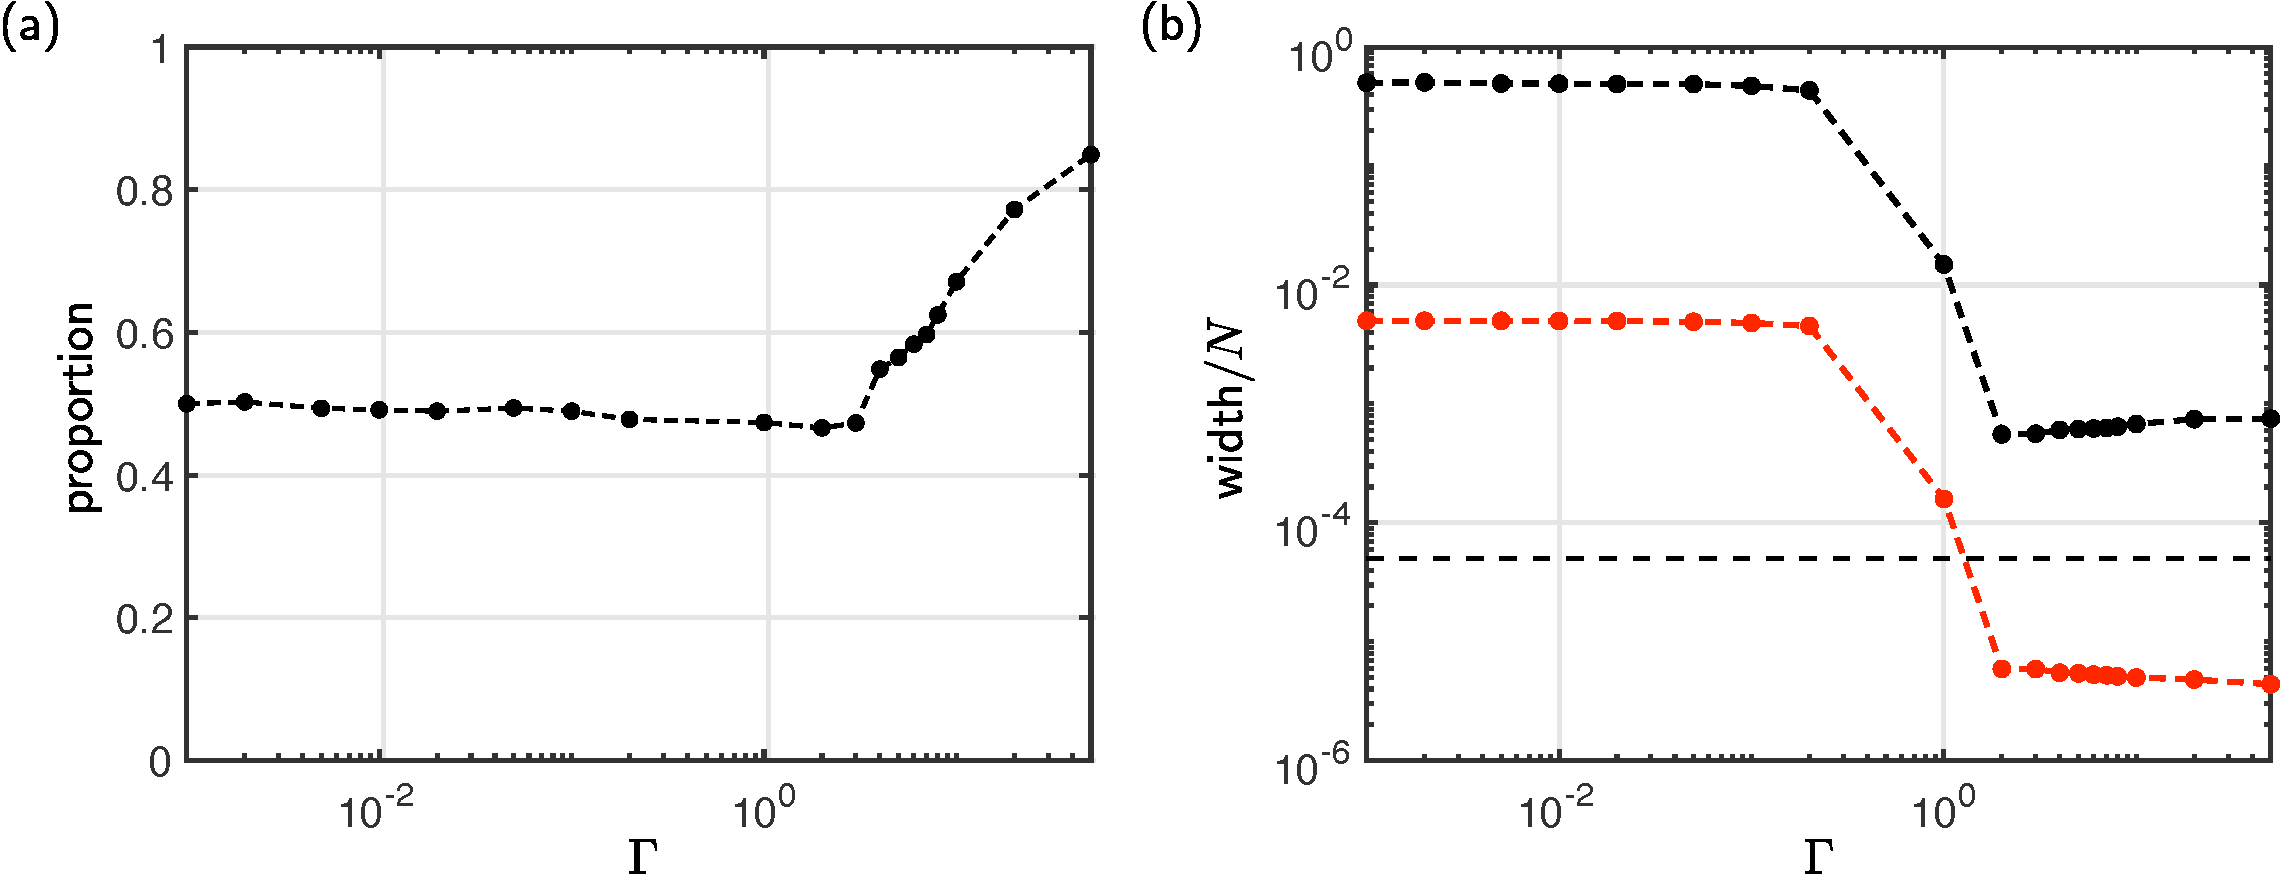
\includegraphics[scale=0.35]{proportion_and_exposed_area}
\caption{(a) Plot of average proportion of drops reaching the free end in numerical solutions of the full equation~\eqref{E:NumSols:MDE:MatrixDifferentialEquation} with random initial conditions~\eqref{E:Numerics:NumericalExperiments:RandomIC}. Each data point is obtained by averaging over 10 solutions, each of which has a different initial condition, with $V_j = 0.3,~ \xbar_0 = 0.5$ and $N = 199$ channels ($200$ plates). In each solution, the proportion of drops reaching the free end is determined at the point at which every drop is at one end of the array or the other. (b) Plot of average exposed (defined in main text) channel widths (red curve) and total width of exposed channels (black curve), both normalised by the array size $N$ (the latter is then the product of proportion of droplets reaching the free end and the mean exposed area). The horizontal dashed black line corresponds to a channel width of $10^{-2}$, the distance at which the van der Waals force is zero. }\label{fig:Discussion:Statistics}
\end{figure}

Having described the clustering behaviour, we now briefly discuss droplet transport (as mentioned in \S\ref{S:Numerics}) and discuss the implications of our findings for removing droplets from an array of channels.

Figure~\ref{fig:Discussion:Statistics}(a) shows that the trend observed in a few numerical solutions in \S\ref{S:Numerics:NumericalExperiments} -- that larger values of $\Gamma$ (stronger surface tension) are associated with a greater proportion of droplets reaching the free end -- is reasonably robust (note that the flattening of the curve at large $\Gamma$ is because of the finite size of the array). This is not true, however, when $\Gamma < 1$;  in this case,  a pairwise mode dominates, and roughly half of the droplets reach the free end and half end up at the opposite end of the array, as we predicted analytically in \S\ref{S:ClusterAnalysis:SmallGamma}.

In terms of droplet removal (our original motivation, as discussed in Chapter 1), we expect that fluid can be removed faster from configurations which have a greater number of droplets at the free end, where they are exposed to the atmosphere. It is tempting, therefore, to conclude that optimising liquid removal would be achieved by taking $\Gamma$ as large as possible -- i.e. making the array as deformable as possible (for a given liquid) -- to maximise the proportion of droplets reaching the free end eventually (Figure~\ref{fig:Discussion:Statistics}(a)). However, this ignores the possibility that removing drops requires access to them: we expect that in general, the smaller the gap at the free end, the harder it will be to remove a droplet.

To quantify this, we define `exposed' channels as those channels that have a droplet at their free end eventually (i.e. when every droplet has reached one end or the array or the other). Figure~\ref{fig:Discussion:Statistics}(b) shows that not only are all of
exposed channels essentially shut for $\Gamma > 1$ (average channel widths at the free end are below the distance at which van der Waals forces become important) -- so individual droplet removal is difficult -- but also that the total width of the exposed channels is smaller in this case too. This is despite a much greater proportion of droplets reaching the free end for $\Gamma > 1$.

We suggest that the choice of $\Gamma$ (and hence the trapping behaviour) may depend on the mechanism for droplet removal: for example, if droplets are to be evaporated out of the array, a configuration which traps droplets, thus preventing exposure to ambient conditions, may be penalised more heavily than one with many drops at the base. On the other hand, droplet removal by coalescence~\citep{Wisdom2013PNAS} would place a premium on droplets reaching the free end, as this mechanism relies on contact with an external droplet.
 This discussion is reminiscent of the flexible case considered in Chapter 2, where droplet transport speed was optimised by taking the corresponding elasto-capillary number $\nu$ as large as possible, albeit with the risk of trapping the droplet. The particulars of this optimisation would depend on the mechanism of removal and is not discussed further here, but may make an interesting extension to the work presented in this chapter.

\section{Non-wetting drops}\label{S:NonWetting}
\begin{figure}
\centering
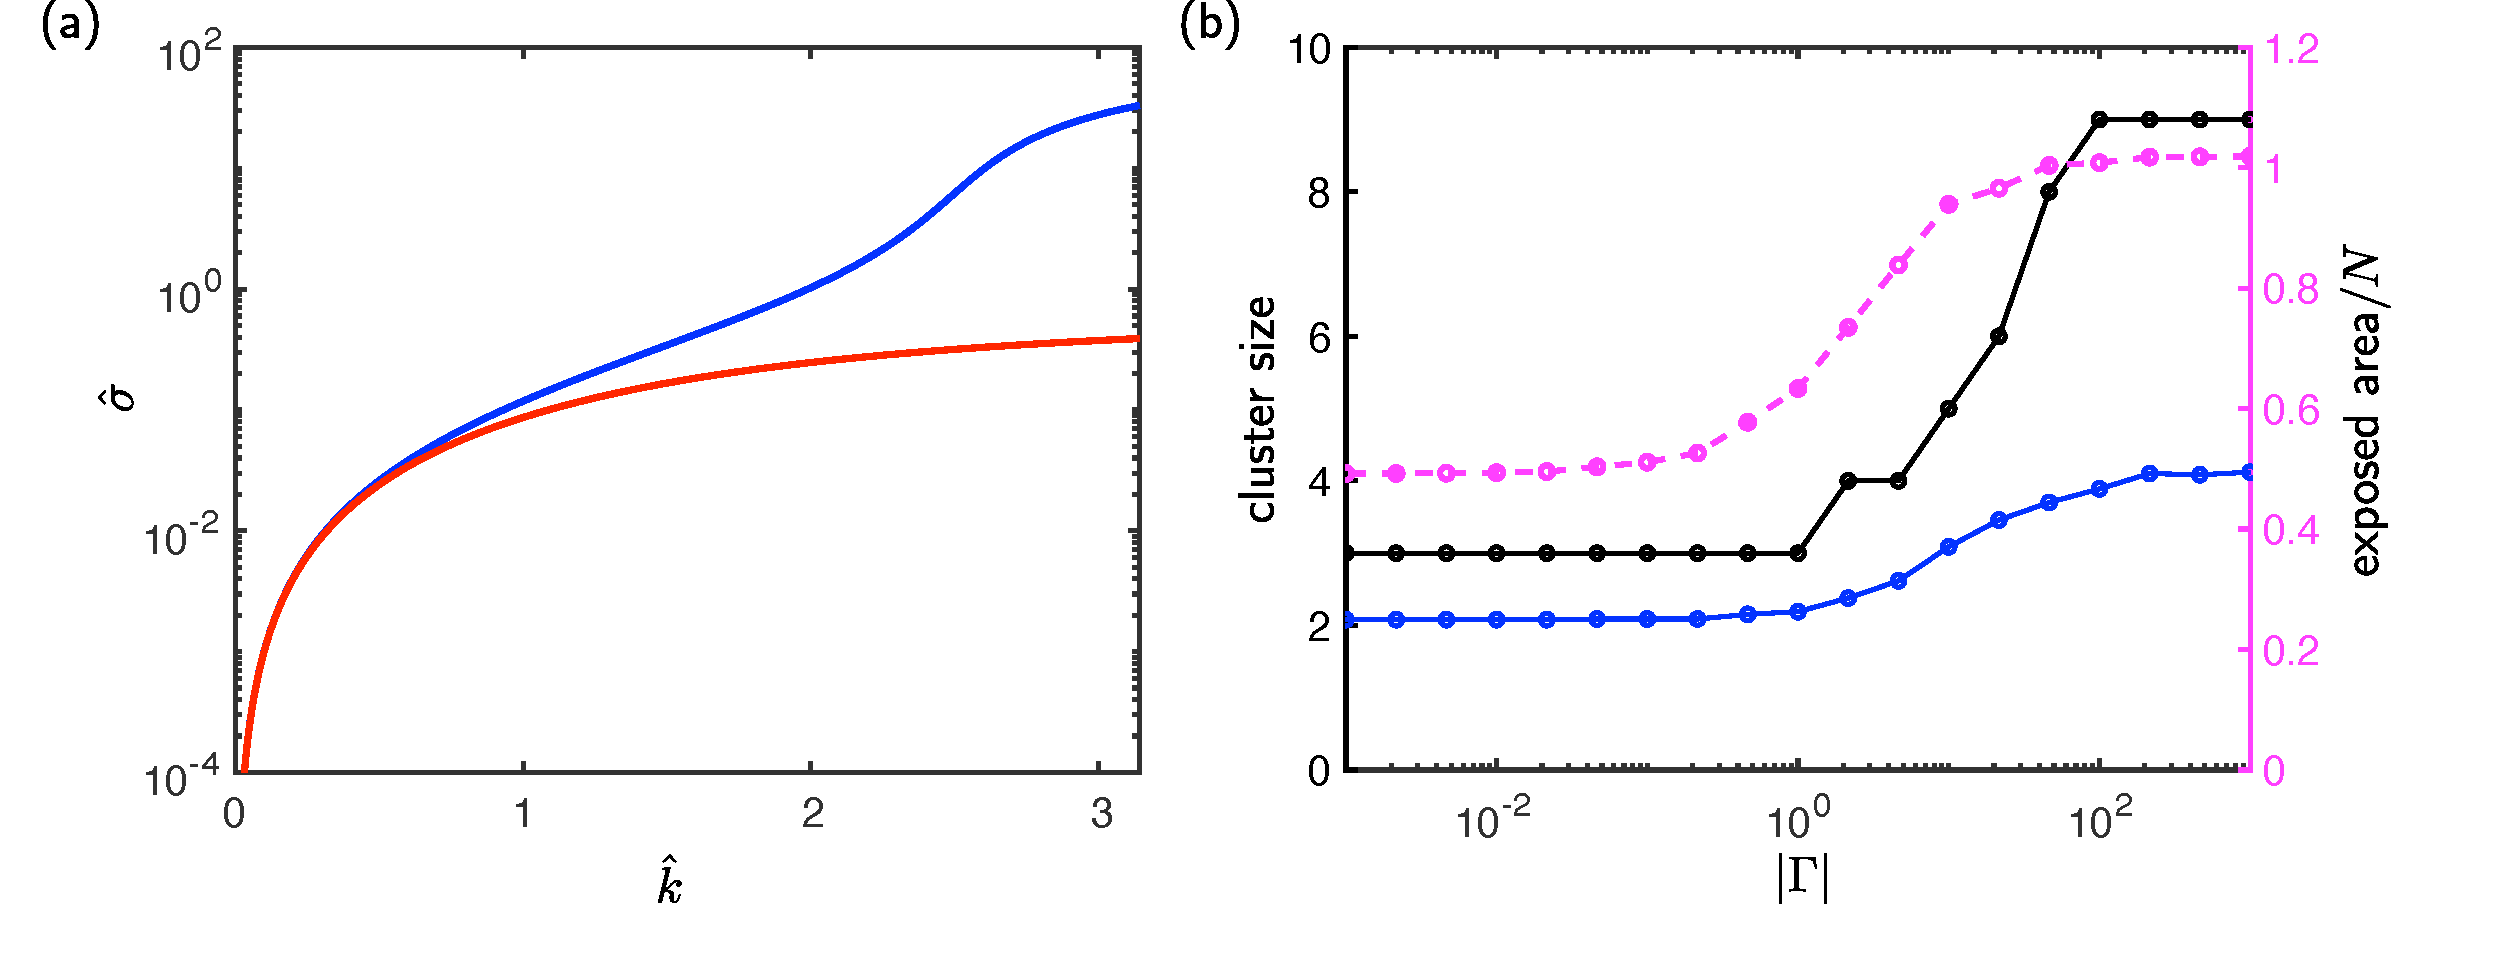
\includegraphics[scale=0.34]{wetting_non_wetting_comparison}
\caption{(a) Growth rates $\hat{\sigma}$ of the unstable modes in the linear analysis as a function of the rescaled wavenumber $\hat{k} = |\Gamma|^{1/2}k$. The red curve is the positive root of equation~\eqref{E:LSA:Continuum:DispersionRelationRescaled} (relevant for non-wetting drops, $\Gamma >0$), and the blue curve is the positive root of equation~\eqref{E:NonWetting:DispersionNonWetting} (relevant for wetting drops, $\Gamma <0$). (b) Mean (blue curve) and maximum (black curve) cluster sizes in a single numerical solution of~\eqref{E:NumSols:MDE:IC} with random initial condition~\eqref{E:Numerics:NumericalExperiments:RandomIC} (here, $\epsilon = 10^{-3}$, $N = 199$, $V = 0.3,~\xbar_0 = 0.5$) and non-wetting conditions ($\Gamma < 0 $). Note that each solution uses the same initial condition. The magenta line indicates the total area of exposed droplets at the moment when every drop has reached one end of the array or the other. } \label{fig:NWD:Comparisons}
\end{figure}
The results of this chapter so far are for wetting droplets ($\Gamma >0$); in this section we briefly discuss the corresponding results for non-wetting drops ($\Gamma < 0$). The results of the linear stability analysis in \S\ref{S:LSA} extend to non-wetting drops: the dispersion has two roots which correspond to one stable and one unstable mode, and the pairwise mode ($N_p = 2$) always has the highest growth rate. It is worth noting however, that the growth rates of the unstable mode are larger for wetting drops than for non-wetting drops. To illustrate this, we compare in Figure~\ref{fig:NWD:Comparisons} the continuous growth rates in the wetting and non-wetting cases, after rescaling the dispersion relation to remove dependence on $\Gamma$ (as described in \S\ref{S:LSA:Continuum}). Explictly, in the non-wetting case, this dispersion relation is
\begin{equation}\label{E:NonWetting:DispersionNonWetting}
\left[C_p + V^3 \left(\frac{V^2}{240} + \frac{\bar{x}_0^2}{4}\right)\hat{k}^2\right]\hat{\sigma}^2 + \left[1 + V\left(\frac{V^2}{6} + 2\bar{x}_0^2\right)\hat{k}^2\right] \hat{\sigma} - \frac{V}{3}\hat{k}^2 = 0.
\end{equation}


We can understand the lack of symmetry (in $\Gamma \to -\Gamma$) by considering the mechanism for instability:  in the wetting case, a perturbation which moves a droplet closer to the free end results in an increased torque applied to the plates containing it, closing the channel and squeezing the droplet as it does so. As a result, the droplet lengthens and the Laplace pressure within it applies over a larger section of channel walls, further increasing the torque applied. In other words, there are two destabilizing effects: the increased torque from moving closer to the free end, and also from the droplet pressure applying over a larger area. In the non-wetting case, however, the increased torque resulting from a perturbation in which a droplet moves closer to the free end acts to widen the channel (the Laplace pressure is positive in the non-wetting case), resulting in a shortening of the droplet and therefore reducing the length over which the Laplace pressure applies. That the growth rate is always positive even for non-wetting drops means that the destabilizing effect of moving closer to the free end always `wins' the competition between these two effects.

The dependence of mean and maximum cluster size on $\Gamma$ displays similar characteristics to wetting drops (note that in the case of non-wetting drops, a channel is said to be part of a cluster if its tapering is positive, $\dthetaj >0$, rather than negative as for the wetting case, since droplets with positive Laplace pressure deform channels outwards). As shown in Figure~\ref{fig:NWD:Comparisons}(b), the system almost always selects a pairwise mode when surface tension is weak. However, for large $\Gamma$, we do not obviously see the $\Gamma^{1/2}$ scaling, but we expect this scaling to pervade at large $\Gamma$ (larger than those shown); the clusters are smaller for non-wetting drops than wetting drops (because of the competing mechanisms described above), so the long wavelength structures for which the $\Gamma^{1/2}$ scaling holds will appear at larger values of $\Gamma$.

One key difference between the wetting and non-wetting cases is droplet removal. Since non-wetting drops move towards the free end in channels which are tapered outwards along their length, channels with droplets at their free ends are open. As a result, the total exposed area increases with $|\Gamma|$ in this case (Figure~\ref{fig:NWD:Comparisons}(b)): for larger $|\Gamma|$, more droplets reach the free end, and the exposed channels are wider. This suggests that the trade-off discussed in \S\ref{S:Discussion} is not necessary for non-wetting drops -- an array can be designed to transport the most liquid to the free end by maximising $|\Gamma|$. Recalling the definition of $\Gamma$ from \S\ref{S:Model:NonDim}, this may be achieved by making the channels long or narrow, or the walls highly compliant. The design of an array for both wetting and non-wetting drops would, however, still be limited by the behaviour for wetting drops.

\section{Summary}
In this chapter, we have considered the interaction between droplets in neighbouring channels, each of which would undergo bendotaxis in isolation. We have developed a mathematical model of this multi-body bendotaxis, in which we assumed for simplicity that the channel walls are rigid and tethered at their base by torsional springs. Our modelling choice of torsional springs was motivated by the behaviour of a single channel, in which wettability-independent droplet transport still occurs, as verified by numerical solutions of the governing equations.

The system has an equilibrium when all of the droplets have equal volume and identical positions in their channels. A linear stability analysis revealed, however, that this equilibria is unstable regardless of the droplet volume and the value of $\Gamma$ --  the parameter that describes strength of surface tension compared to spring stiffness -- and the system will, therefore, always move away from this equilibrium. This suggests that droplet mobility may be an important aspect of elasto-capillary clustering, since previous studies of similar systems in which droplets are pinned at one end of the array have equilibria that are unstable only when surface tension is sufficiently strong~\citep{Singh2014JFM, Hadjittofis2016JFM}. %good for the water strider because it never gets stuck in the worst case scenario for this simplified geometry

%linear stability says pairwise most unstable but numerical solutions have array of sizes
Although the linear stability analysis suggests that the pairwise mode is that fastest growing, we observed a range of cluster sizes in an ensemble of numerical solutions of the model equations with random initial conditions. This range depends sensitively  on the value of the parameter $\Gamma$. For small surface tension, a pairwise mode was almost always observed because the deflection angles (and thus direction of droplet motion) is set simply by the difference in the position of droplets across the channel walls. We rationalized this result by analyzing the governing ODEs in the case of small deflections that is associated with the limit $\Gamma \to 0$. For strong surface tension $\Gamma \gg 1$, however, a distribution of cluster sizes are observed, with a maximal size that scales with $\Gamma^{1/2}$. By using a discrete-to-continuum approximation of the ODEs, we suggested that this appears to be the result of the propagation of fronts through the system which `lock in' clusters of this set size; with a random initial condition, these fronts interact with one another to `smooth out' the cluster sizes between the pairwise mode preferred by the linear stability analysis and the maximal cluster size set by the front propagation.

Finally, we discussed the implications of our model for self-cleaning surfaces exploiting bendotaxis. The ensemble of numerical solutions revealed that for $\Gamma \lesssim 1$, approximately half of the droplets reach the free end, and half end up at the base of the array, in accord with a pairwise separations, and that the proportion of droplets reaching the free end is increasing for $\Gamma \gtrsim 1$. However, this increasing proportion of droplets reaching the free end is to weighed against the fact that the channels are almost closed, thus making droplet removal potentially difficult.

%experiment, but we have ignored condensation
Returning to the question posed at the start of the chapter, the work in this chapter suggests that the pairwise mode observed in the condensation experiments of Figure 5.1 is not generic behaviour in multi-body bendotaxis, and larger clusters may be observed experimentally for more deformable arrays. We note, however, that in this experiment the droplet volume is varied dynamically (via condensation), an effect that has been observed to exert a strong influence on elasto-capillary clustering by~\cite{Hadjittofis2016JFM}; understanding the influence of dynamically changing droplet volume on bendo-capillary clustering would make an interesting extension to the work presented in this chapter.

\begin{subappendices}
%\appendix
%\addcontentsline{toc}{section}{Appendices}
\renewcommand{\thesection}{\Alph{section}}
\section{Governing equations as a system of ordinary differential equations}\label{Appendix:Reduction}

In this appendix, we describe how to express the governing equations derived in \S\ref{S:Model:NonDim} as a system of ODEs. We first consider unpinned droplets and then subsequently discuss pinned droplets. Here, all variables are non-dimensional and hats have been dropped.\newline
It is convenient to work in terms of the drop half lengths and mean positions, defined as
\begin{equation}\label{A:E:Reductions:xbar_ell_definition}
\ellj = \frac{\xrightj - \xleftj}{2}\quad\text{and}\quad \xbarj = \frac{\xrightj + \xleftj}{2},
\end{equation}
respectively. The governing equations and boundary conditions, (equations~\eqref{E:Model:NonDim:ReynoldsEq}, \eqref{E:Model:NonDim:Kinematic}, \eqref{E:Model:NonDim:Laplace}, and~\eqref{E:Model:NonDim:TorqueBalance} in the main text), in terms of~\eqref{A:E:Reductions:xbar_ell_definition}, the drop pressures $p_j$, deflection angles $\theta_{j+1/2}$ and their derivatives are
\begin{align}\label{A:Eq:Reduction:Reynolds}
x\dd{\left(\dthetaj\right)}{t} &= \frac{1}{3|\Gamma|}\ddp{ }{x}\left[h_j^3 \ddp{p_j}{x}\right],& &\text{for}~\xbarj -\ellj < x < \xbarj + \ellj,
\end{align}
\begin{align}
& C_p\dd{\theta_{j+1/2}}{t} + \theta_{j+1/2} = \int^{\xbarj + \ellj}_{\xbarj - \ellj} x p_j~\mathrm{d}x -  \int^{\bar{x}_{j+1}+ \ell_{j+1}}_{\bar{x}_{j+1}- \ell_{j+1}} x p_{j+1}~\mathrm{d}x +\tau^{\text{vdw}}_{j+1/2},\label{A:Eq:Reduction:Torque}\\
&\dd{\left(\xbar_j \pm \ell_j\right)}{t} = -\left.\frac{h_j^2}{3|\Gamma|}\ddp{p_j}{x}\right|_{x = \xbar_j \pm \ell_j},\label{A:Eq:Reduction:Kinematic}\\
&p_j(x = \xbar_j \pm \ell_j, t) = -\frac{\Gamma}{h_j^{\pm}}\label{A:Eq:Reduction:PressureBC},
\end{align}
where $h_j(x,t) = 1 +x \dthetaj$ is the $j^{\text{th}}$ channel width, $\dthetaj =\theta_{j+1/2}- \theta_{j-1/2}$,  and $h_j^{\pm} = h_j(x_j^{\pm}), \bar{h}_j = h_j(\xbar_j)$. The droplet lengths are related to the deflection angles and mean positions via the droplet volumes
\begin{equation}\label{A:Eq:Reduction:Volume}
V_j = 2\ell_j(1 + \xbar_j \dthetaj),
\end{equation}
which must be constant throughout (thus the $\ell_j$ are known functions of $\xbar_j$ and $\dthetaj$); these volumes are set by initial conditions
\begin{equation}\label{A:Eq:Reduction:IC}
\xbar_j(0) = \xbar_j^0 = \frac{x_{j,0}^+ + x_{j,0}^-}{2}, \quad \theta_{j+1/2}(0) = \theta_{j+1/2}^0
\end{equation}

Recall that the index $j$ runs from $j = 1$ to $j = N$, with periodic conditions imposed by specifying that variables with subscripts $0$ and $N+1$ are equal to the same variable with subscript $N$ and $1$, respectively.

Integrating Reynolds' equation~\eqref{A:Eq:Reduction:Reynolds} gives\begin{equation}\label{A:E:Reduction:IntegratedReynolds}
\frac{\xbar_j^2 - x^2}{2}\dd{(\dthetaj)}{t}  =-\frac{h_j^3}{3|\Gamma|}\ddp{p_j}{x} - \bar{Q}_j,
\end{equation}
where
\begin{equation}\label{A:E:Reduction:MidptFlux}
\bar{Q}_j(t) =- \left.\frac{\bar{h}_j^3}{3|\Gamma|}\ddp{p_j}{x}\right|_{x = \xbar_j}
\end{equation}
is the depth averaged flux of fluid through the mean-meniscus position~\citep{Leal2007} (referred to henceforth as the mean-point flux). Rearranging~\eqref{A:E:Reduction:IntegratedReynolds} gives the pressure gradient in terms of the mean-point flux:
\begin{equation}\label{A:E:Reduction:PressureGradient}
\ddp{p_j}{x} = \frac{3|\Gamma|}{2h_j^3}\left[(x^2 - \xbar_j^2) \dd{(\dthetaj)}{t} - 2\bar{Q}_j\right].
\end{equation}
Integrating this expression  over the whole drop gives the pressure change between the two menisci:
\begin{equation}\label{A:E:Reduction:PressureJump1}
\left[p_j\right]^{\xbar_j + \ell_j}
_{\xbar_j - \ell_j}= \frac{3(I^2_j - \xbar_j^2 I^0_j)|\Gamma|}{2}\dd{(\dthetaj)}{t} - 3|\Gamma|\bar{Q}_j I^0_j.
\end{equation}
where we recall that the integrals $I_j^n$ are defined by
\begin{equation}\label{A:E:Reduction:InDefinition}
I_j^n(x,t) = \int_{\xbar_j - \ell_j}^{\xbar_j + \ell_j} \frac{x^n}{h_j^3}~\mathrm{d}x, ~n \in \mathbb{N}.
\end{equation}

 A second expression for the pressure change between the menisci is obtained by taking the difference of the boundary conditions~\eqref{A:Eq:Reduction:PressureBC}:
\begin{equation}\label{A:E:Reduction:PressureJump2}
\left[p_j\right]^{\xbar_j + \ell_j}_{\xbar_j - \ell_j}=\frac{2 \Gamma\ell_j \dthetaj}{h_j^+ h_j^-}.
\end{equation}
Equating~\eqref{A:E:Reduction:PressureJump1} and~\eqref{A:E:Reduction:PressureJump2} gives the mean point flux
\begin{equation}\label{A:E:Reduction:Midpt_Flux1}
\bar{Q}_j = \frac{I_2^j - \xbar_j^2 I_0^j}{2I_0^j}\dd{(\dthetaj)}{t} - \frac{2\ell_j \dthetaj \sgn (\Gamma)}{3h_j^+ h_j^-}.
\end{equation}
 The terms on the right hand side of~\eqref{A:E:Reduction:Midpt_Flux1} represent fluid flux arising from the squeezing of the droplet and tapering of the channel, respectively. Note that at this point we have the droplet pressure $p_j$ in terms of $\Delta \theta_j$, $\xbar_j$ and their derivatives by integrating~\eqref{A:E:Reduction:PressureGradient} alongside one of the pressure boundary conditions~\eqref{A:Eq:Reduction:PressureBC} (but this is not used in the what follows).

Inserting~\eqref{A:E:Reduction:Midpt_Flux1} into~\eqref{A:Eq:Reduction:Kinematic} and~\eqref{A:E:Reduction:PressureGradient} gives a set of $N$ ODEs:
\begin{multline}\label{A:Eq:Reduction:ODESet1}
2\dd{\xbarj}{t}  +\frac{1}{2} \left[\frac{\ellj^2 + 2\ellj \xbarj}{h_j^+} + \frac{\ellj^2 - 2\ellj \xbarj}{h_j^-} -  \frac{I_2^j - \xbar_j^2 I_0^j}{I_0^j} \left(\frac{1}{h_j^+} + \frac{1}{h_j^-}\right)\right]\dd{(\dthetaj)}{t} =\\
-\frac{2\ellj\dthetaj\sgn(\Gamma)}{3I_0^j h_j^+ h_j^-} \left(\frac{1}{h_j^+} + \frac{1}{h_j^-}\right).
\end{multline}

Now we consider the torque balance~\eqref{A:Eq:Reduction:Torque}, in which the integrals (the contributions to the hydrodynamic torque) on the right hand side must be evaluated.  Although the droplet pressures are now known, it is more convenient to evaluate these after first integrating by parts:
\begin{equation}\label{A:E:Reduction:HydrodynamicTorqueIBP}
\int^{\xbarj + \ellj}_{\xbarj - \ellj} x p_j~\mathrm{d}x=  \left[\frac{x^2}{2}p_{j}\right]_{\xbar_{j} - \ell_{j}}^{\xbar_{j}+\ell_j} -\int^{\bar{x}_{j}+ \ell_{j}}_{\bar{x}_{j}- \ell_{j}} \frac{x^2}{2} \ddp{p_{j}}{x}~\mathrm{d}x.
\end{equation}
Inserting~\eqref{A:Eq:Reduction:PressureBC},~\eqref{A:E:Reduction:PressureGradient}  and~\eqref{A:E:Reduction:Midpt_Flux1} into~\eqref{A:E:Reduction:HydrodynamicTorqueIBP}, we find
\begin{equation}\label{A:E:Reduction:HydrodynamicTorqueIBP2}
\int^{\xbarj + \ellj}_{\xbarj - \ellj} x p_j~\mathrm{d}x  = \frac{\Gamma}{2}\left[  \frac{2\ell_{j}\Delta \theta_{j}I^2_j}{ h_j^+ h_j^- I^0_j}           +   \frac{(\bar{x}_{j}+\ell_{j})^2}{h_{j}^+} - \frac{(\bar{x}_{j}-\ell_{j})^2}{h_{j}^-}          \right] - |\Gamma|\viscdamp_j\ddp{\Delta \theta_{j}}{t}
\end{equation}
where
\begin{equation}\label{A:Eq:Reduction:ViscDampDefn}
\viscdamp_j = \frac{3}{4I^0_j}\left[I^0_j I^4_j - \left(I^2_j\right)^2\right]
\end{equation}
which can be interpreted as damping arising from droplet viscosity.

Inserting~\eqref{A:E:Reduction:HydrodynamicTorqueIBP2} into~\eqref{A:Eq:Reduction:Torque} gives a set of $N$ ODEs
\begin{multline}
-C_p\dd{\theta_{j+1/2}}{t} + \viscdamp_{j+1}|\Gamma|\dd{\Delta \theta_{j+1}}{t} -  \viscdamp_{j}|\Gamma|\dd{\Delta \theta_{j}}{t} =\\
\theta_{j+1/2} - \tau^{\text{vdW}}_{j+1/2} + \frac{\Gamma}{2}\left[\frac{2\ell_{j}\Delta \theta_{j}I^2_j}{ h_j^+ h_j^-I^0_j} - \frac{2\ell_{j+1}\Delta \theta_{j+1}I^2_{j+1}}{ h_{j+1}^+ h_{j+1}^-I^0_{j+1}} -\right. \\
\left.\frac{(\bar{x}_{j+1}+\ell_{j+1})^2}{h_{j+1}^+} + \frac{(\bar{x}_{j+1}-\ell_{j+1})^2}{h_{j+1}^-} + \frac{(\bar{x}_{j}+\ell_{j})^2}{h_{j}^+} - \frac{(\bar{x}_{j}-\ell_{j})^2}{h_{j}^-}\right].\label{A:Eq:Reduction:ODESet2}
\end{multline}
Equations~\eqref{A:Eq:Reduction:ODESet1} and~\eqref{A:Eq:Reduction:ODESet2}
are a set of $2N$ ordinary differential equations in $\xbar_j, \theta_{j+1/2}$, which are to be solved alongside initial conditions~\eqref{A:Eq:Reduction:IC}.

\subsection{Pinned droplets}
When any droplet is pinned, the governing equations still reduce to a set of $2N$ ODEs. However, the pressure within pinned drops is different to unpinned drops, so the kinematic equations~\eqref{A:Eq:Reduction:ODESet1} and hydrodynamic torques~\eqref{A:E:Reduction:HydrodynamicTorqueIBP}  are modified in this case; in this section we briefly describe these modifications. Note that when a droplet is pinned, equations Reynolds equation~\eqref{A:Eq:Reduction:Reynolds} and the kinematic conditions~\eqref{A:Eq:Reduction:Kinematic} still hold, so that equations~\eqref{A:E:Reduction:MidptFlux}--\eqref{A:E:Reduction:PressureJump1} for the midpoint flux, pressure gradient and pressure jump from the previous section still hold.

\subsubsection{Droplets Pinned at $x = 1$}
If the $j^{\th}$ droplet is pinned at $x = 1$, we impose pressure boundary conditions on the pressure (replacing~\eqref{A:Eq:Reduction:PressureBC})
\abeqn{A:E:Reduction:Pinned:PinnedTopBC}{\left.p_j \right|_{x =  \xbar_j - \ell_j} = -\frac{\Gamma}{h_j^{-}},\qquad \left.\ddp{p_j}{x}\right|_{x =  \xbar_j + \ell_j = 1} = 0.}
Evaluating~\eqref{A:E:Reduction:IntegratedReynolds} at $\xbar_j + \ell_j=1$, and using~\eqref{A:E:Reduction:Pinned:PinnedTopBC}b we find the mean-point flux to be
\begin{equation}\label{A:E:Reduction:Pinned:Top:MidptFlux}
\bar{Q}_j = \frac{1 - \xbar_j^2}{2}\dd{\Delta \theta_{j}}{t}.
\end{equation}
The pressure gradient within the drop is then (using~\eqref{A:E:Reduction:PressureGradient})
\begin{equation}\label{A:E:Reduction:Pinned:Top:PressureGradient}
\ddp{p_j}{x} = \frac{3|\Gamma|}{2h_j^3}\left(x^2 - 1\right)\dd{\Delta \theta_{j}}{t},
\end{equation}
and the pressure jump (using~\eqref{A:E:Reduction:PressureJump1}) is
\begin{equation}\label{A:E:Reduction:Pinned:Top:PressureJump}
\left[p_j\right]^{\xbar_j + \ell_j}
_{\xbar_j - \ell_j} = \frac{3|\Gamma|}{2}\left(I_j^2 - I_j^0\right)\dd{\Delta \theta_{j}}{t}.
\end{equation}
Hence, taking the sum of the kinematic conditions~\eqref{A:Eq:Reduction:Kinematic} gives
\begin{equation}\label{A:E:Reduction:Pinned:Top:KinematicEquations}
\dd{\xbar_j}{t} = \frac{\xbar_j\ell_j}{h_j^-}\dd{\Delta \theta_{j}}{t}.
\end{equation}
This replaces~\eqref{A:Eq:Reduction:ODESet1} if the $j^{\th}$ drop is pinned at $x = 1$.

To evaluate the hydrodynamic torque contribution from this droplet, we first note that
\begin{equation}\label{A:E:Reduction:Pinned:Top:IBPhelp}
\left[x^2 p_j\right]^{\xbar_j + \ell_j}
_{\xbar_j - \ell_j} = \left[x^2 \right]^{\xbar_j + \ell_j}
_{\xbar_j - \ell_j}p_j(\xbar_j -\ell_j,t) + (\xbar_j + \ell_j)^2\left[ p_j\right]^{\xbar_j + \ell_j}
_{\xbar_j - \ell_j},
\end{equation}
in which both terms on the right hand side are known. After integrating by parts, and using~\eqref{A:E:Reduction:Pinned:Top:PressureGradient} and~\eqref{A:E:Reduction:Pinned:Top:IBPhelp} we find that, for a drop pinned at $x = 1$,
\begin{equation}\label{A:E:Reduction:Pinned:Top:HydrodynamicTorque}
\int^{\xbarj + \ell_j}_{\xbar_j - \ell_j} x p_j~\mathrm{d}x  =\int^{1}_{\xbarj - \ellj} x p_j~\mathrm{d}x= -\frac{2\Gamma\xbar_j \ell_j}{h_j^-} - |\Gamma|C_j^{d,p_1}\ddp{\Delta \theta_{j}}{t},
\end{equation}
where
\begin{equation}
C_j^{d,p_1} = I_j^4 + I_j^0 - 2I_j^2
\end{equation}
is the damping from droplet viscosity in this case. Expression~\eqref{A:E:Reduction:Pinned:Top:HydrodynamicTorque} replaces~\eqref{A:E:Reduction:HydrodynamicTorqueIBP2} when the $j^{\th}$ drop is pinned at $x = 1$ (and therefore changes~\eqref{A:Eq:Reduction:ODESet2}, the resulting equations are contained in Appendix~\ref{Appendix:MatrixDifferentialEquation}).
\subsubsection{Droplets Pinned at $x = 0$}
Similarly, if the $j^{\th}$ droplet is pinned at $x = 0$, the boundary conditions
\abeqn{A:E:Reduction:Pinned:Bottom:BC}{\left.\ddp{p_j}{x}\right|_{x =  \xbar_j - \ell_j = 0} = 0,\qquad \left.p_j \right|_{x =  \xbar_j +\ell_j} = -\frac{\Gamma}{h_j^{+}}}
replace~\eqref{A:Eq:Reduction:PressureBC}. Following the same procedure as in the previous subsection, we find that the kinematic equations~\eqref{A:Eq:Reduction:ODESet1} should be replaced by
\begin{equation}\label{A:E:Reduction:Pinned:Bottom:KinematicEquations}
\dd{\xbar_j}{t} =- \frac{\xbar_j\ell_j}{h_j^+}\dd{\Delta \theta_{j}}{t},
\end{equation}
 in this case. The hydrodynamic torque contribution from this droplet is
 \begin{equation}
 \int^{\xbarj + \ell_j}_{\xbar_j - \ell_j} x p_j~\mathrm{d}x  = \int^{\xbarj + \ell_j}_{0} x p_j~\mathrm{d}x = -\frac{2\Gamma\xbar_j \ell_j}{h_j^+} - |\Gamma|C_j^{d,p_1}\dd{\Delta \theta_{j}}{t},
\end{equation}
where
\begin{equation}
C_j^{d,p_0} = I_j^4
\end{equation}
is the damping from droplet viscosity in this case.

\section{Weak surface tension: $|\Gamma | \ll 1$}\label{Appendix:SmallGammaAnalysis}
\newcommand{\smallpar}{|\Gamma|} %to prevent confusion, define small parameter.
\newcommand{\angl}{\phi}
\newcommand{\dangl}{\Delta \angl}
In this appendix, an asymptotic analysis is presented for the case of weak surface tension $|\Gamma | \ll 1$. Here, we consider only unpinned droplets. Weak surface tension is associated with small deformations, so we scale
\begin{equation}\label{A:E:SmallGamma:ScaledAngles}
\theta_{j+1/2} = \smallpar \angl_{j+1/2}.
\end{equation}
The channel widths,
\begin{equation}\label{A:E:SmallGamma:ChannelWidths}
h_j = 1 +x (\theta_{j+1/2} - \theta_{j-1/2}) = 1 + x\smallpar (\angl_{j+1/2} - \angl_{j+1/2}),
\end{equation}
are then unity to leading order in $\smallpar$ (the assumption of small deformations holds only when $\angl_{j+1/2} = \mathcal{O}(1)$ -- this is verified a posteriori).

Using the notation $\Delta \angl_j = \angl_{j+1/2} - \angl_{j-1/2}$, the drop volumes are
\begin{equation}\label{A:E:SmallGamma:Volumes}
V_j = 2\ell_j(1 + \smallpar \Delta \angl_j) =2\ellj + \mathcal{O}(\smallpar),
\end{equation}
i.e. the drop lengths are half of the droplet volumes, $\ell_j = V_j/2$, to leading order in $\smallpar$.

The integrals $I_j^n$ can be expanded in $\smallpar$ as
\begin{equation*}
I_j^n = \int_{\xbarj - \ellj}^{\xbarj + \ellj} \frac{x^n}{(1 + x\smallpar \dangl)^3} ~\mathrm{d}x= \frac{1}{n+1}\left[\left(\xbar_j + \frac{V_j}{2}\right)^{n+1} - \left(\xbar_j -\frac{V_j}{2
} \right)^{n+1}\right] + \mathcal{O}(\smallpar),
\end{equation*}
and therefore
\begin{equation}\label{A:E:SmallGamma:IntegralExpansionsI}
\viscdamp_j = \frac{3\left[I^0_j I^4_j - (I^2_j)^2\right]}{4I^0_j} = V_j^3\left(\frac{V_j^2}{240} + \frac{\xbar_j^2}{4}\right) +\mathcal{O}(\smallpar).
\end{equation}
The first term on the right hand side is the leading order contribution to viscous damping and is denoted by $\viscdamp_{j,0}$. Similarly, we find that
\begin{equation}\label{A:E:SmallGamma:IntegralExpansionsII}
\frac{I_2^j - \xbar_j^2 I_0^j}{2I_0^j} = \frac{V_j^2}{24} + \mathcal{O}(\smallpar).
\end{equation}

Recall the expression for the mean-point flux
\begin{equation}\label{A:E:SmallGamma:Midpt_Flux1}
\bar{Q}_j = \frac{I_2^j - \xbar_j^2 I_0^j}{2I_0^j}\dd{(\dthetaj)}{t} - \frac{2\ell_j \dthetaj \sgn (\Gamma)}{3h_j^+ h_j^-},
\end{equation}
derived in the Appendix~\ref{Appendix:Reduction}. When the displacements are small, this becomes
\begin{align}
\bar{Q}_j = \smallpar \left[\frac{V_j^2}{24} \dd{(\dangl_j)}{t} - \frac{V_j \dangl_j \sgn (\Gamma)}{3 }  \right]+ \mathcal{O}(\smallpar^2).\label{A:E:SmallGamma:MidptFlux}
\end{align}
This shows that the mean-point fluxes are small ($\mathcal{O}(\smallpar)$) on an $\mathcal{O}(1)$ time scale, and motivates defining a fast time scale
\begin{equation}\label{A:E:SmallGamma:ShortTime}
T = t/\smallpar.
\end{equation}
On this time scale the mean-point fluxes are proportional to the rate at which the channel closes:
\begin{equation}\label{A:E:SmallGamma:ShortTimeFlux}
\bar{Q}_j(T) = \frac{V_j^2}{24}\dd{\left(\dangl_{j}\right)}{T} + \mathcal{O}(\smallpar).
\end{equation}
Only the first term of~\eqref{A:E:SmallGamma:MidptFlux} -- corresponding to the squeezing of the droplet by the channel walls -- contributes significantly to the mean-point fluxes on this fast time scale.

Inserting the scalings~\eqref{A:E:SmallGamma:ScaledAngles} and~\eqref{A:E:SmallGamma:ShortTime} into the kinematic equations~\eqref{A:Eq:Reduction:Kinematic}, we find that
\begin{align}
\left[2 + \mathcal{O}(\smallpar)\right]\bar{Q}_j(T) &= \frac{2}{\smallpar}\dd{\xbar_j}{T} + \left[V +\mathcal{O}(\smallpar)\right]\dd{(\dangl)}{T}\label{A:E:SmallGamma:ShortTimeFluxI}\\
\implies \dd{\xbar_j}{T} &= \mathcal{O}(\smallpar),\label{A:E:SmallGamma:ShortTimeFluxII}
\end{align}
meaning that droplets do not move appreciably on this time scale.

Inserting the scalings~\eqref{A:E:SmallGamma:ScaledAngles} and~\eqref{A:E:SmallGamma:ShortTime} into the torque balance~\eqref{A:Eq:Reduction:ODESet2} gives
\begin{multline}\label{A:E:SmallGamma:TorqueBalance}
-C_p\dd{\angl_{j+1/2}}{T} +\viscdamp_{j+1,0}\dd{(\dangl_{j+1})}{T} -\viscdamp_{j,0}\dd{(\dangl_{j+1})}{T} =\\ \angl_{j+1/2} - \sgn(\Gamma)\left(V_{j+1} \xbar_{j+1}  - V_j \xbar_j\right)+\mathcal{O}(\Gamma),
\end{multline}
where $\viscdamp_{j,0}$ are constant on this fast time scale (as the $\xbar_j$ are constant). Equations~\eqref{A:E:SmallGamma:TorqueBalance} can be expressed in matrix form as
\begin{equation}\label{A:E:SmallGamma:MatrixDE_ShortTimescale}
\underline{C}_{\text{fast}}\dd{\underline{\phi}}{T} = \underline{\phi} -  \sgn(\Gamma) \underline{u},
\end{equation}
where
\begin{multline*}\label{A:E:SmallGamma:ViscousDampingMatrix}
\underline{C}_\text{fast} =\\  \begin{bmatrix}
-(C_p+\viscdamp_{1,0} +\viscdamp_{2,0}) & \viscdamp_{2,0}   & & & \viscdamp_{1,0} \\
\viscdamp_{2,0} & -(C_p+\viscdamp_{2,0} +\viscdamp_{3,0}) & \viscdamp_{3,0}  \\
 & \viscdamp_{3,0} & \ddots & \ddots \\
& & \ddots & \ddots & \viscdamp_{N,0} \\
\viscdamp_{1,0}& & &\viscdamp_{N,0}&- (C_p+\viscdamp_{N,0} +\viscdamp_{1,0})
\end{bmatrix},
\end{multline*} and $\underline{u} = (V_1\xbar_1,\dots, V_N\xbar_N)^\intercal$. Note that $\underline{C}_\text{fast}$ is constant, so the behaviour of solutions to~\eqref{A:E:SmallGamma:MatrixDE_ShortTimescale} is given by the eigenvalues of $\underline{C}_\text{fast}$. As $\underline{C}_\text{fast}$ is Hermitian and strictly diagonally dominant\footnote{A matrix is diagonally dominant if, for every row in the matrix, the absolute value of the diagonal entry in that row is larger than the sum of the absolute value of all other entries in that row.} with negative entries on its diagonal, it is negative definite -- i.e. all of its eigenvalues are negative. Therefore, solutions to~\eqref{A:E:SmallGamma:MatrixDE_ShortTimescale} decay in time to a quasi-equilibrium set by the net droplet torque across the beam:
\begin{equation}\label{A:E:SmallGamma:FastTimescaleSolution}
\phi_{j+1/2}^{\text{eq}}=\phi_{j+1/2}(T\to \infty)= \sgn(\Gamma) u_j =\sgn(\Gamma) \left( V_{j+1}\xbar_{j+1} - V_j \xbar_j\right).
\end{equation}
In particular, at early times ($t \lesssim \mathcal{O}(\Gamma)$) -- when the mean-meniscus positions are equal to their initial values to leading order in $|\Gamma|$ -- the deflection angles evolve to an equilibrium
\begin{equation}
\phi_{j+1/2} ^{\text{eq},0} = \sgn(\Gamma) \left( V_{j+1}\xbar_{j+1}^0 - V_j \xbar_j^0\right),
\end{equation}
where $\xbar_j^0 = \xbar_j(0)$. At later times, the  deflection angles are given by $\phi^{\text{eq}}_{j+1/2}$.


\begin{figure}[t]
\centering
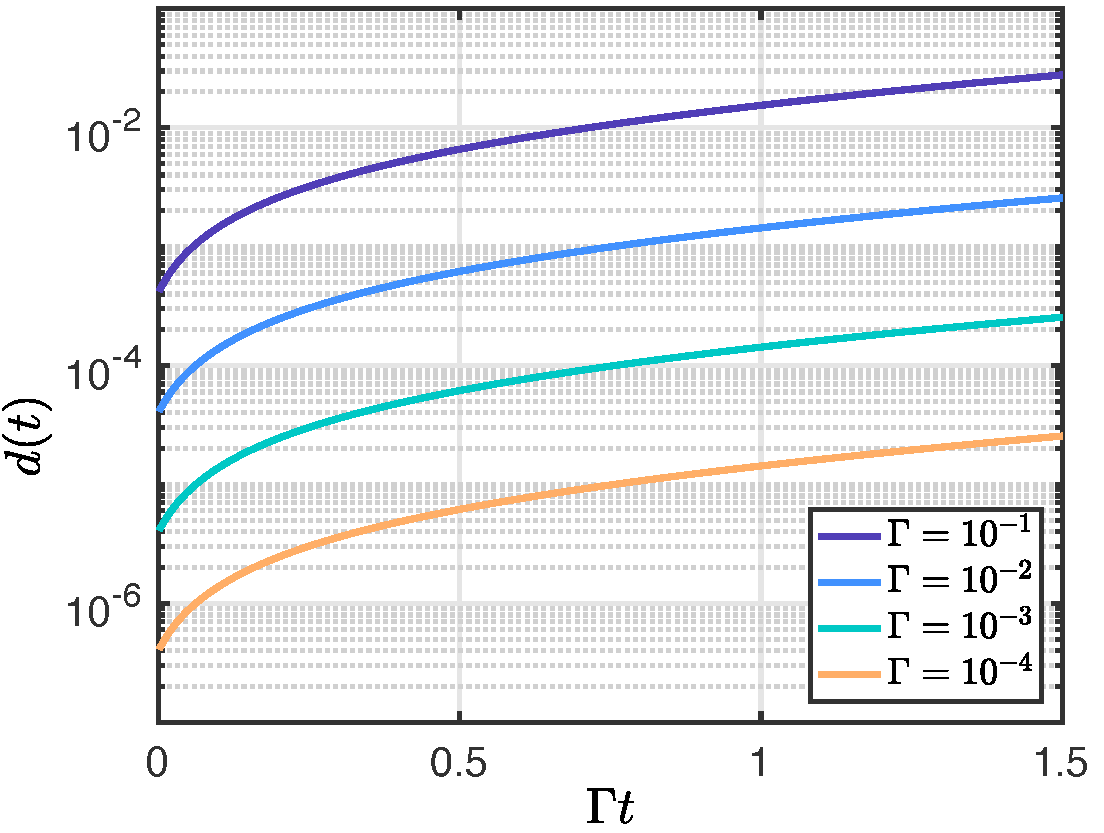
\includegraphics[scale=0.47]{Small_gamma_comparison_labelled}
\caption{Plot of $d =   ||\underline{\bar{x}}- \underline{\bar{x}}_{\text{num}}||_2$ -- the difference between
numerical solutions of~\eqref{E:NumSols:MDE:MatrixDifferentialEquation} and the approximation~\eqref{A:E:SmallGamma:xbar_solution} valid for weak surface tension ($|\Gamma|\ll 1$) as a function of $\Gamma t$ on semi-logarithmic axes (to facilitate comparison between different values of $\Gamma$). Here, $N = 199$, and the initial conditions (used in both the numerical solutions and asymptotic approximations) are $\xbar_j= 0.5 + 0.02 \mathcal{R}_j$, where the $\mathcal{R}_j$ are random numbers sampled from a normal distribution with zero mean and unity variance. The numerical solutions also have initial conditions $\theta_{j+1/2}(0) = 0$. Each curve corresponds to a different value of $\Gamma$ as described in the legend (the same initial conditions are used for each curve). Note that the $d(0) = 0$ in each case, but this is not resolved on the scale plotted here (the solution~\eqref{A:E:SmallGamma:xbar_solution} only describes the behaviour on long timescales). Note that a droplet reaches the end of the channel at $\Gamma t \approx 1.6$ in the numerical solutions (beyond which point the analysis of Appendix~\ref{Appendix:SmallGammaAnalysis} is no longer valid).} \label{fig:Appendix:SmallGamma:ManyChannelAgreement}
\end{figure}


The dynamics of the droplet motion are determined from the kinematic ODEs. Recall that on an $\mathcal{O}(1)$ time scale they are
\begin{multline}\label{A:E:SmallGamma:Kinematic}
2\dd{\xbarj}{t}  +\frac{1}{2} \left[\frac{\ellj^2 + 2\ellj \xbarj}{h_j^+} + \frac{\ellj^2 - 2\ellj \xbarj}{h_j^-} -  \frac{I_2^j - \xbar_j^2 I_0^j}{I_0^j} \left(\frac{1}{h_j^+} + \frac{1}{h_j^-}\right)\right]\dd{(\dthetaj)}{t} +\\
\frac{2\ellj\dthetaj\sgn(\Gamma)}{3I_0^j h_j^+ h_j^-} \left(\frac{1}{h_j^+} + \frac{1}{h_j^-}\right) = 0.
\end{multline}
In the case of small displacements, the second term and third terms (those in $\mathrm{d}(\Delta \theta_j)/\mathrm{d}t$ and $\Delta \theta_j$, respectively) are $\mathcal{O}(\smallpar)$. To determine droplet motion, we therefore rescale onto a long time scale by introducing
\begin{equation}\label{A:E:SmallGamma:SlowTimescaleDefn}
T_{s} = \smallpar t.
\end{equation}
Inserting~\eqref{A:E:SmallGamma:SlowTimescaleDefn}, and the original small deflection scalings~\eqref{A:E:SmallGamma:ScaledAngles}, \eqref{A:E:SmallGamma:ChannelWidths}, and~\eqref{A:E:SmallGamma:FastTimescaleSolution} into~\eqref{A:E:SmallGamma:Kinematic} gives, at leading order,
\begin{equation}
\dd{\xbar_j}{T_s} =- \sgn(\Gamma)\frac{\phi_{j+1/2}^\text{eq} - \phi_{j-1/2}^\text{eq}}{3} =- \frac{V_{j+1}\xbar_{j+1} - 2V_j \xbar_{j} + V_{j-1}\xbar_{j-1}}{3}.
\end{equation}
As a matrix differential equation, this is
\begin{equation}\label{A:E:SmallGamma:xbar_equation}
\dd{\underline{\xbar}}{T_s} = -\frac{1}{3}\partial^2\underline{V}~\underline{\xbar}
\end{equation}
where $\underline{\xbar} = \left(\xbar_1,\dots, \xbar_N\right)^{\intercal}$ and
\begin{equation}\label{A:E:SmallGamma:VolumeMatrix}
\partial^2\underline{V} =  \begin{bmatrix}
-2V_1 & V_2   & & & V_N \\
V_1 & -2V_2 & V_3  \\
 & V_2 & \ddots & \ddots \\
& & \ddots & \ddots & V_N \\
V_1& & &V_{N-1}&- 2V_N
\end{bmatrix},
\end{equation}
resembles the Laplacian operator but weighted by the drop volumes. The matrix problem~\eqref{A:E:SmallGamma:xbar_equation} is to be solved alongside the initial condition $\underline{\xbar}(0) = \underline{\xbar}^0 =  (\xbar_1^0,\dots, \xbar_N^0)^\intercal$.

In general, there is no analytic expression for the eigenvalues of $\partial^2\underline{V} $ and the problem~\eqref{A:E:SmallGamma:xbar_equation} must be solved numerically. However, when all the droplet volumes are equal ($V_j = V$ for all $j$, as considered in \S\ref{S:ClusterAnalysis}), the matrix $\partial^2\underline{V}$ is proportional to the periodic Laplacian matrix $D^2$ (defined in~\eqref{E:ClusterSizes:SmallGamma:LongTimescaleMatrix}), and has eigenvalues
\begin{equation}\label{A:E:SmallGamma:Eigenvalues}
\lambda_p =\left\{
 \begin{array}{ll}
- 4V\sin^2\left(\frac{\pi(p-1)}{2N}\right) & p \text{~odd,}\\
- 4V\sin^2\left(\frac{\pi p}{2N} \right) & p\text{~even.}\\
 \end{array}\right.
\end{equation}
With the exception of the zero ($p = 1$) eigenvalue, and the largest eigenvalue if $N$ is even, the eigenvalues are repeated and each eigenspace has rank two. The orthonormal eigenvectors of $D^2$ are denoted by $\underline{v}_p$ whose $q^{\text{th}}$ component is given by
\begin{equation}\label{A:E:SmallGamma:Eigenvectors}
\underline{v}_{p,q} =N^{-1/2} \times\left\{
 \begin{array}{ll}
1&  \text{if}~p = 1,\\
 (-1)^q   & \text{if}~p = N ~ \text{and} ~ N ~\text{is even,}\\
\sqrt{2}\sin \left(\frac{\pi(q-1/2)p}{N}\right) & \text{otherwise, with}~p ~ \text{even,} \\
  \sqrt{2}\cos \left(\frac{\pi(q-1/2)(p-1)}{N}\right) & \text{otherwise, with}~p ~ \text{odd.} \\
  \end{array}\right.
\end{equation}
The solution of~\eqref{A:E:SmallGamma:xbar_equation}  with $\underline{\xbar}(0) =\underline{\xbar}^0$ is
\begin{equation}\label{A:E:SmallGamma:xbar_solutionLongTime}
\underline{\xbar} = \sum_{p=1}^{N} (\underline{\xbar}^0.\underline{v}_p)\underline{v}_p\exp\left(-\frac{\lambda_p}{3} T_s\right),
\end{equation}
or, in terms of the original timescale,
\begin{equation}\label{A:E:SmallGamma:xbar_solution}
\underline{\xbar} = \sum_{p=1}^{N} (\underline{\xbar}^0.\underline{v}_p)\underline{v}_p\exp\left(-\frac{\lambda_p}{3}  \smallpar t\right).
\end{equation}
To compare the solution~\eqref{A:E:SmallGamma:xbar_solution} to numerical solutions of the full equations~\eqref{E:NumSols:MDE:MatrixDifferentialEquation} with the same initial conditions (denoted by $\underline{\xbar}_{\text{num}}$) we define the difference between the solutions to be
\begin{equation}
d(t) =  ||\underline{\bar{x}}- \underline{\bar{x}}_{\text{num}}||_2.
\end{equation}
Figure~\ref{fig:Appendix:SmallGamma:ManyChannelAgreement} shows that $d(t) \to 0$ as $\Gamma \to 0$, indicating agreement between~\eqref{A:E:SmallGamma:xbar_solution} and numerical solutions of the full equations~\eqref{E:NumSols:MDE:MatrixDifferentialEquation}.

\subsection{Single channel case}
\begin{figure}[t]
\centering
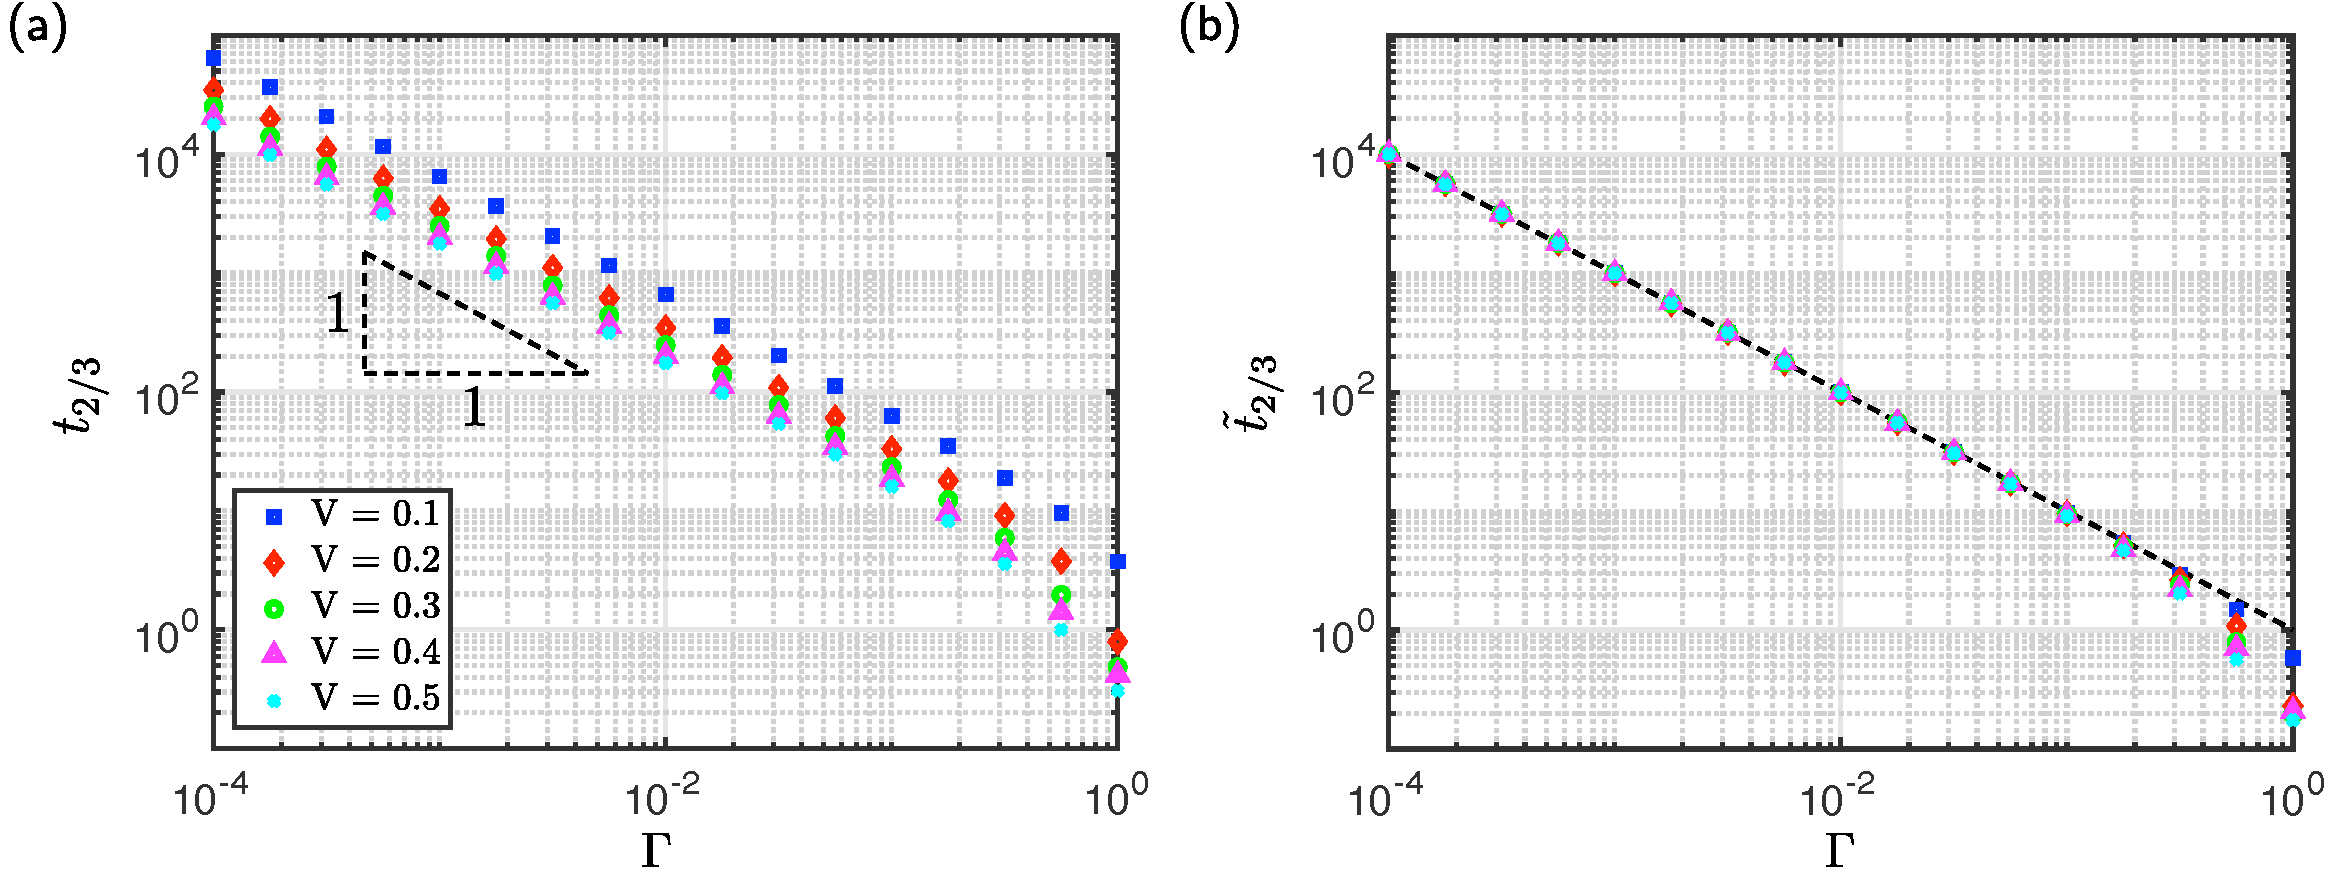
\includegraphics[width = \textwidth]{single_channel_Asymptotics_combined.pdf}
\caption{Plot of $t_f$, the time between $x^+ = \xbar + \ell = f$ and $x^+ = \xbar + \ell = 1$ determined by solving numerically the equations~\eqref{E:TwoPlates:DAEs1}--\eqref{E:TwoPlates:DAEs2} with initial conditions $\theta_0 = 0, \xbar_0 = 0.4$ (note that $t_f$ is approximately independent of initial condition, as droplet inertia is neglected). (a) Numerical results of $t_{2/3}$ for various droplet volumes (symbols, see legend). Note that solutions are only presented for $\Gamma > 0$. (b) Collapse of the numerical results in (a) when rescaled according by taking $\tilde{t}_{2/3} = 2Vt_{2/3}/\left[3 \log((2-V)/(4/3-V)\right]$ (equation~\eqref{A:E:SmallGamma:TwoPlatesBendotaxisTime}). The dashed black line indicates the asymptotic prediction  $\tilde{t}_{2/3}  = \Gamma^{-1}$.}\label{fig:Appendix:SmallGamma:SingleChannelAgreement}
\end{figure}

The analysis of this section so far holds for $N\geq 3$. In the case of the single drop-channel system discussed in \S\ref{S:SingleChannel} -- which is equivalent to setting $N=2$ and considering one of the two drops (say $j = 2$) to have trivial volume --
the behaviour in the limit $|\Gamma|\to 0$ can be found, however, by repeating the analysis with only slight modification. As discussed in \S\ref{S:SingleChannel}, the single channel case requires us to consider only a single angle $\theta = \theta_{3/2}$ and its mean meniscus position $\xbar$ (its length $\ell$ is specified by the volume constraint); following the steps of the previous section, we find that the angles are set on the same fast ($\mathcal{O}(\smallpar)$) time scale, with the scaled angle $\phi = \theta/\smallpar$ evolving according to
\begin{equation}\label{A:E:SmallGamma:TwoPlates:ShortTime}
\left(C^{d,0} + C_p\right)\dd{\phi}{T} =-\left[ \sgn(\Gamma)V\xbar+ \phi\right],
\end{equation}
where $C^{d,0}$ is the leading order contribution to the viscous damping of the relevant drop (constant on this time scale, as before). The deflection angle is quasi-static on any longer time scale, and given by $\phi = \phi^{\text{eq}} = -\sgn(\Gamma)V\xbar$.

The drop moves on a long ($\mathcal{O}(1/\smallpar)$) timescale; its mean position evolves according to
\begin{equation}
\dd{\xbar}{t} = \frac{2V|\Gamma|}{3}.
\end{equation}
Solving this alongside the initial condition $\xbar(0) = \xbar_0$ (this is the appropriate initial condition because droplet does not move appreciably during the fast time scale) gives
\begin{equation}\label{A:E:SmallGamma:TwoPlatesXbarSol}
\xbar(t) = \xbar_0 \exp\left(\frac{2V|\Gamma|}{3}t\right).
\end{equation}
To compare this result with numerical solutions of the governing equations~\eqref{E:TwoPlates:DAEs1}--\eqref{E:TwoPlates:DAEs2}, we invert expression~\eqref{A:E:SmallGamma:TwoPlatesXbarSol} to find $t_f$, the time between $x^+ = \xbar + \ell = f$ and $x^+ = \xbar + \ell = 1$:
\begin{equation}\label{A:E:SmallGamma:TwoPlatesBendotaxisTime}
t_f = \frac{3}{2|\Gamma|V}\log \left(\frac{2-V}{2f-V}\right).
\end{equation}
The agreement between~\eqref{A:E:SmallGamma:TwoPlatesBendotaxisTime} and $t_f$ determined by numerically solving the governing equations can be seen in Figure~\ref{fig:Appendix:SmallGamma:SingleChannelAgreement}.


\section{Matrix differential equation}\label{Appendix:MatrixDifferentialEquation}
To facilitate their numerical solution, the governing equations~\eqref{E:Model:DAEs:TorqueBal} and~\eqref{E:Model:DAEs:Kinematic} (and the modifications for pinned drops, as described in Appendix~\ref{Appendix:Reduction}) are first expressed as a matrix differential equation.

Using the notation $\underline{\theta} = \left(\theta_{3/2},\dots, \theta_{N+1/2}\right)^\intercal$, $ \underline{\bar{x}} = \left(\xbar_1,\dots, \xbar_N\right)^\intercal$, the torque balance equations~\eqref{E:Model:DAEs:TorqueBal} read
\begin{equation}\label{A:E:MDE:TorqueBalance}
\left(-C_p\mathbb{I }_N+ |\Gamma| D^2 \underline{C}^d\right)\dd{\underline{\theta}}{t} = \underline{\theta} - \underline{\tau}_{\text{VDW}} - \Gamma D \underline{F}( \underline{\theta},  \underline{\xbar}).
\end{equation}
Here, $\mathbb{I}_N$ denotes the $N \times N$ identity matrix and $\underline{\tau}^{\text{vdW}} = (\tau^{\text{vdW}}_{3/2},\dots, \tau^{\text{vdW}}_{N+1/2})^\intercal$ are the van der Waals forces on the beams.  Also
\begin{equation}\label{A:E:MDE:ViscousLaplacian}
D^2 \underline{C}^d =  \begin{bmatrix}
-(C^d_1 +C^d_2) & C^d_2   & & & \viscdamp_1 \\
C^d_2 & -(C^d_2 +C^d_3) & C^d_3  \\
 & C^d_3 & \ddots & \ddots \\
& & \ddots & \ddots & C^{d,i}_N \\
C^d_1& & &C^d_N&- (C^d_{N} +C^d_{1})
\end{bmatrix},
\end{equation}
describes the damping arising from droplet viscosity (empty entries are filled with zeros), in which
\begin{equation}
C^{d}_j = \begin{cases}
I_j^4 + I_j^0 - 2I_j^2 & \text{if the}~j^{\th}~\text{droplet is pinned at} ~ x = 1,\\
I_j^4 &\text{if the}~j^{\th}~\text{droplet is pinned at} ~ x = 0,\\
\left[I_j^0 I_j^4 - \xbar_j^2 (I_2^j)^2\right]/I_j^0 &\text{otherwise}.
\end{cases}
\end{equation}
The matrix
\begin{equation}
D =  \begin{bmatrix}
-1 & 1  & & & \\
 & -1& 1  \\
& & -1& \ddots &\\
& &  & \ddots &1  \\
1& && &-1
\end{bmatrix},
\end{equation}
captures the difference across channels and $\underline{F}$ describes the hydrodynamic torque due to each droplet. If the droplet is not pinned, the  $j^{\text{th}}$ entry of $\underline{F}$ is
\begin{align}
F_j &=\frac{-\ell_{j}\Delta \theta_{j}I^2_j}{ h_j^+ h_j^-I^0_j}  + \frac{(\bar{x}_{j}+\ell_{j})^2}{2h_{j}^+} - \frac{(\bar{x}_{j}-\ell_{j})^2}{2h_{j}^-},
\label{A:E:MDE:F_definition}
\end{align}
whilst its $j^{\text{th}}$ entry is
\begin{equation}
F_j =\frac{-2\Gamma \xbar_j \ell_j}{h_j^+}, \quad \text{or}  \quad F_j=  \frac{-2\Gamma \xbar_j \ell_j}{h_j^-}
\end{equation}
for droplets pinned at $x = 1$ or droplets pinned at $x = 0$, respectively.

The matrix representation of the kinematic conditions~\eqref{E:Model:DAEs:Kinematic} is
\begin{equation}\label{A:E:MDE:Kinematic}
2\dd{\underline{\bar{x}}}{t} +\underline{G}(\underline{\theta},  \underline{\xbar})D\dd{\underline{\theta}}{t} =\sgn(\Gamma) \underline{H}(\underline{\theta},  \underline{\xbar}).
\end{equation}
$\underline{H}$ describes the contribution to drop motion arising from drop imbibition into a tapered channel:
\begin{equation}\label{A:E:MDE:H_definition}
\underline{H}_j =\left\{\begin{array}{ll}
0 & \text{if the}~j^{\th}~\text{droplet is pinned at either end},\\
-\frac{2\ellj\dthetaj}{3I_0^j h_j^+ h_j^-} \left(\frac{1}{h_j^+} + \frac{1}{h_j^-}\right) & \text{otherwise}.
\end{array}\right.
\end{equation}
$G$ describes how the droplets move in response to channel closure:
\begin{equation*}
\underline{G}_j =\left\{\begin{array}{ll}
-\frac{\xbar_j \ell_j}{h_j^-} &j^{\th}~\text{drop pinned at} ~ x = 1,\\
\frac{\xbar_j \ell_j}{h_j^+} & j^{\th}~\text{drop pinned at} ~ x = 0,\\
\frac{1}{2} \left[\frac{\ellj^2 + 2\ellj \xbarj}{h_j^+} + \frac{\ellj^2 - 2\ellj \xbarj}{h_j^-} -  \frac{I_2^j - \xbar_j^2 I_0^j}{I_0^j} \left(\frac{1}{h_j^+} + \frac{1}{h_j^-}\right)\right] & \text{otherwise}\end{array}\right.
\end{equation*}
Combining~\eqref{A:E:MDE:TorqueBalance} and~\eqref{A:E:MDE:Kinematic} gives a single matrix differential equation in $\underline{u} =  (\underline{\theta}^\intercal, \underline{\bar{x}}^\intercal)^\intercal$:
\begin{equation}\label{A:E:MDE:MatrixDifferentialEquation}
\underline{M}\dd{\underline{u}}{t} =\underline{f},
\end{equation}
where
\begin{equation}\label{A:E:MDE:MassMatrix}
\underline{M} = \left(
\begin{array}{cc}
-\hat{C}\mathbb{1}_n + |\Gamma| D^2 \underline{C}^d & \underline{0}_{N} \\
\underline{G}~ \underline{D} & 2\mathbb{1}_{N}
\end{array}
\right)
\end{equation}
and
\begin{equation}\label{A:E:MDE:Forcing}
\underline{f} =  \left( \begin{array}{c} \underline{\theta} - \underline{\tau}^{\text{vdW}} + \Gamma \underline{F}\\ \sgn(\Gamma) \underline{H}\end{array}\right)
\end{equation}
play the roles of a mass matrix and force, respectively.

\end{subappendices}
